%%This is a very basic article template.
%%There is just one section and two subsections.
\documentclass[12pt,openright]{memoir}

\usepackage{charter}
\usepackage{courier}
%\usepackage[scaled]{helvet}
%\renewcommand{\ttdefault}{pcr}
\normalfont % in case the EC fonts aren't available
\usepackage[T1]{fontenc}

\usepackage{graphicx}
\usepackage[colorlinks]{hyperref}
\usepackage{listings}
\usepackage{setspace}
\usepackage{pdflscape}
\usepackage{soul}
\usepackage{color}
\usepackage{longtable}
\usepackage{multirow}
\usepackage{eso-pic}
\usepackage{rotating}
\usepackage{subscript}
\usepackage{tikz}

\newcommand\BackgroundPic{
\put(-4,0){
\parbox[b][\paperheight]{\paperwidth}{%
\vfill
\centering

\includegraphics[width=\paperwidth,height=\paperheight,
keepaspectratio]{background.png}%
\vfill
}}}

%!TEX root = ../EpsilonBook.tex

\lstset{escapeinside={/*@}{@*/}}
\definecolor{codebackground}{rgb}{0.95,0.95,0.95}
\lstset{backgroundcolor=\color{codebackground}}

\lstset{
  captionpos=b,
  numberstyle=\tiny,
  basicstyle=\ttfamily\footnotesize,
  columns=flexible,
  tabsize=2,
  numbers=left,
  nolol=true
}

\lstdefinelanguage{EOL}{
morekeywords={delete,import,for,while,in,and,or,self,operation,return,def,var,throw,if,new,else,transaction,abort,
break,breakall,continue,assert,assertError,not, switch, case, default},
sensitive=true,
morecomment=[l]{//},
morecomment=[s]{/*}{*/},
morestring=[b]",
showstringspaces=false
}
\lstdefinelanguage{ECL}{
morekeywords={pre, post, do, import, var, auto, abstract, rule, extends, not, with, guard, match, for, in, and, or, self, operation, return, def, if, new, else, match, compare, conform, into},
sensitive=true,
morecomment=[l]{--},
%morecomment=[s]{/*}{*/},
morestring=[b]',
showstringspaces=false
}

\lstdefinelanguage{ETL}{
morekeywords={import, pre, post, var, rule, to, extends, not, with, guard, match, merge, transform, for, in, and, or, self, operation, return, def, if, new, else, match, compare, conform, into},
sensitive=true,
morecomment=[l]{--},
%morecomment=[s]{/*}{*/},
morestring=[b]',
showstringspaces=false
}

\lstdefinelanguage{EPL}{
morekeywords={active,import,pre,post,var,pattern,match,onmatch,nomatch,do,from,in,guard,not,with,guard,match,merge,transform,for,in,and,or,self,operation,return,def,if,new,else,match,compare,conform,into},
sensitive=true,
morecomment=[l]{//},
morestring=[b]',
morestring=[b]",
showstringspaces=false
}

\lstdefinelanguage{EML}{
morekeywords={import, pre, post, mid, var, auto, abstract, rule, to, extends, not, with, guard, match, merge, transform, for, in, and, or, self, operation, return, def, if, new, else, match, compare, conform, into, switch, case, default},
sensitive=true,
morecomment=[l]{//},
morecomment=[s]{/*}{*/},
morestring=[b]",
showstringspaces=false
}

\lstdefinelanguage{EWL}
{morekeywords={import, wizard, guard, do, title, for, not, in, and, or, operation, return, var, def, if, new, else},
sensitive=true,
morecomment=[l]{--},
%morecomment=[s]{/*}{*/},
morestring=[b]',
showstringspaces=false,
}

\lstdefinelanguage{EVL}
{morekeywords={for, import, pre, post, context, kindOf, high, medium, low, constraint, critique, check, do, message, title, fix, not, guard, in, and, or, operation, return, var, def, if, new, else, delete, switch, case, default},
sensitive=true,
morecomment=[l]{//},
morecomment=[s]{/*}{*/},
morestring=[b]",
showstringspaces=false,
}

\lstdefinelanguage{EOL}{
morekeywords={import,not,for,in,and,or,self,operation,return,def,var,throw,if,new,else},
sensitive=true,
morecomment=[l]{--},
%morecomment=[s]{/*}{*/},
morestring=[b]',
showstringspaces=false
}
\lstdefinelanguage{Flock}
{morekeywords={for, import, migrate, ignoring, when, original, migrated, typeOf, kindOf, do, not, in, and, or, xor, operation, return, var, if, new, else, delete, retype, to, pre, post},
sensitive=true,
morecomment=[l]{//},
morecomment=[s]{/*}{*/},
morestring=[b]",
showstringspaces=false,
}
\lstdefinelanguage{OCL2}{
morekeywords={context, package,endpackage,end,inv,and,or,xor,implies,if,else,then,endif,let,def},
sensitive=true,
morecomment=[l]{--},
%morecomment=[s]{/*}{*/},
morestring=[b]',
showstringspaces=false
}
\lstdefinelanguage{MOFScript}
{morekeywords={rule,to,from,do,result},
sensitive=false,
morecomment=[l]{--},
%morecomment=[s]{/*}{*/},
morestring=[b]',
showstringspaces=false
}

\newsubfloat{figure}

\title{\fontfamily{put}\selectfont{\huge{\bfseries{Epsilon}}}}
\author{
Dimitrios S. Kolovos, Richard F. Paige, \\Louis M. Rose and Fiona A.C. Polack\\\\ 
Department of Computer Science,\\\\The University of York\\\\\\
Antonio Garc\'{\i}a-Dom\'{\i}nguez,\\\\University of C\'adiz (Spain)
}
\date{\today}

% number up to subsections
\setsecnumdepth{subsection}

%two column float page must be 90% full
\renewcommand\dblfloatpagefraction{.99}
%two column top float can cover up to 80% of page
\renewcommand\dbltopfraction{.99}
%float page must be 90% full
\renewcommand\floatpagefraction{.99}
%top float can cover up to 80% of page
\renewcommand\topfraction{.99}
%bottom float can cover up to 80% of page
\renewcommand\bottomfraction{.99}
%at least 10% of a normal page must contain text
\renewcommand\textfraction{.01}

\newcommand*{\eol}[1]{\texttt{#1}}
\newcommand*{\eolannotation}[1]{\eol{#1}}
\newcommand*{\anttarget}[1]{\textit{#1}}
\newcommand*{\xmlattribute}[1]{\textit{#1}}
\newcommand*{\xmlelement}[1]{\textit{\textless{}#1\/\textgreater{}}}

\newcommand*{\class}[1]{\textsc{#1}}
\newcommand*{\method}[1]{\textit{#1}}
\newcommand*{\test}[1]{\textit{#1}}
\newcommand*{\variable}[1]{\textit{#1}}
\newcommand*{\modelname}[1]{``#1''}
\newcommand*{\file}[1]{\texttt{#1}}
\newcommand*{\javaannotation}[1]{\texttt{@#1}}

\begin{document}
\pagestyle{empty}
\AddToShipoutPicture*{\BackgroundPic}
\phantom{invisible}
\clearpage 
Last update: \today{}.
\cleardoublepage
\pagestyle{plain}
\mbox{}
\OnehalfSpacing
%\maketitle

\tableofcontents
\listoffigures
\listoftables

\chapter{Introduction}
\label{chp:Introduction}

The purpose of this book is to provide a complete reference of the languages provided by the Epsilon project (\url{http://www.eclipse.org/gmt/epsilon}). The first version of this book is based on a cut-down version of the first author's PhD thesis so its style may be a bit different than other books on programming languages you may have read so far - but this will hopefully improve in future versions.

\section{What is Epsilon?}

Epsilon, standing for Extensible Platform of Integrated Languages for mOdel maNagement, is - as it's extended name hints - a platform for building consistent and interoperable task-specific languages for model management tasks such as model transformation, code generation, model comparison, merging, refactoring and validation.

Epsilon currently provides the following languages:

\begin{itemize}
	\item Epsilon Object Language (EOL)
	\item Epsilon Validation Language (EVL)
	\item Epsilon Transformation Language (ETL)
	\item Epsilon Comparison Language (ECL)
	\item Epsilon Merging Language (EML)
	\item Epsilon Wizard Language (EWL)
	\item Epsilon Generation Language (EGL)
\end{itemize}

For each language Epsilon provides Eclipse-based development tools and an interpreter\footnote{The interpreters are not bound in any way with Eclipse and can also be used in standalone Java applications.} that can execute programs written in this language. Epsilon also provides a set of ANT tasks for creating workflows of different tasks (e.g. a validation followed by a transformation followed by code generation). The following chapters present the syntax of each language and a few usage examples.

\section{How To Read This Book}

If you are reading this book, there are good chances that you are already interested in using a particular task-specific language provided by Epsilon (e.g. EVL for model validation or EWL for refactoring). In this case, you don't have to need to read about all the languages: you first need to spend some time reading Chapter \ref{chp:InstallingEpsilon} in order to find out how to install Epsilon and Chapter \ref{sec:Design.EOL} that presents the core Epsilon Object Language (EOL), as all languages of the platform extend EOL both syntactically and semantically. Then you can proceed to the chapter that discusses the particular language you are interested in (e.g. Chapter \ref{sec:EVL} for EVL).

\section{Questions and Feedback}

Our intention is to keep this book a live project that will evolve in parallel with the evolution of Epsilon. Therefore, your feedback on any omissions, errors or outdated content is critical and much appreciated (and also you will win a place for your name in the Acknowledgements section of the book :D ). Please send your feedback to the Eclipse eclipse.epsilon newsgroup under news.eclipse.org. If you are not sure about how to connect and post to the newsgroup please refer to \url{http://wiki.eclipse.org/index.php/Webmaster_FAQ#How_do_I_access_the_Eclipse_newsgroups.3F} for detailed instructions.

\section{Additional Resources}

As mentioned above, information about Epsilon and examples are available in many different places. If you can't find what you are looking for in this book there are a few other places where you may try.

\subsection{Epsilon Eclipse GMT}
Epsilon is a component of the Eclipse Modelling GMT project and it is hosted in \url{http://www.eclipse.org/gmt/epsilon}. In the documentation section \url{http://www.eclipse.org/gmt/epsilon/doc} there is documentation about several features of Epsilon, and the Cinema \url{http://www.eclipse.org/gmt/epsilon/cinema} contains a number of Flash screencasts that demonstrate different languages and tools of Epsilon in action.

\subsection{EpsilonLabs}

EpsilonLabs is a satellite project of Epsilon that hosts experimental applications/extensions of Epsilon or other content that cannot be shared under Eclipse.org due to licensing issues (e.g. incompatibility with EPL). EpsilonLabs is located in \url{http://epsilonlabs.sf.net}

\subsection{Epsilon Weblog}
In November 2007 we started a blog where we've been reporting new applications and extensions of Epsilon. The blog provides the latest information on the project and is located in \url{http://epsilonblog.wordpress.com}

%\chapter{Installing Epsilon}
\label{chp:InstallingEpsilon}

There are two options for installing Epsilon. Through the Eclipse Update Manager or by checking out the source code from the Eclipse SVN and (if you'd like to play with experimental stuff) EpsilonLabs SVN servers. This chapter provides detailed instructions for both installation options.

\section{Prerequisites}

You first need to install the following software before you can install Epsilon.

\begin{enumerate}
	\item Java 1.5 (or later)
	\item Eclipse 3.3 (or later)
	\item EMF 2.3 (or later) 
	\item GMF 2.0 (or later) (optional)
	\item Emfatic (optional) (recommended)
\end{enumerate}

The Java runtime can be downloaded from \url{http://java.sun.com}. The easiest way to download Eclipse, EMF and GMF together is the Eclipse Ganymede Modeling distribution \url{http://www.eclipse.org/downloads/packages/eclipse-modeling-tools-includes-incubating-components/ganymeder}.

Emfatic is a textual notation for specifying ECore metamodels. It is highly recommended that you install it as all the exemplar metamodels in this book will be progressively specified using it (as opposed to using UML-like diagrams). Emfatic can be installed using the Eclipse Update Manager (a detailed description follows) using the update site : \url{http://epsilonlabs.svn.sourceforge.net/svnroot/epsilonlabs/org.eclipse.emf.emfatic.updatesite/}

\section{Installing using the Eclipse Update Manager/P2}

To install Epsilon using the Eclipse Update Manager please follow the instructions below:

\begin{enumerate}
	\item Go to Help->Software Updates
 	\item In the dialog that pops up press Add Site�
	\item In the dialog that pops up enter  \url{http://download.eclipse.org/modeling/gmt/epsilon/updates} in the URL field.
	\subitem In addition to the main update site above, there is also an interim site which hosts the current (but potentially unstable) version of Epsilon: \url{http://download.eclipse.org/modeling/gmt/epsilon/interim}
	\item Press OK
	\item In the next screen select Epsilon and press Next
	\subitem If you don't have GMF installed, expand the Epsilon node and deselect the Epsilon GMF Support feature
	\item Review the Feature Licence and if you agree select the I accept the terms in the licence agreement and press Next
	\item Press Finish
	\item Eclipse prompts for a restart. Press Yes
\end{enumerate}

\section{Checking out the Source Code from CVS/SVN}

\begin{enumerate}
	\item Switch to the SVN Repository Exploring perspective (from the Window$\rightarrow$Open Perspective$\rightarrow$Other menu)
	\item Click the New Repository Location button on the SVN Repositories view and enter the following configuration details
	\subitem URL : http://dev.eclipse.org/svnroot/modeling/org.eclipse.gmt.epsilon/
	\subitem User : anonymous
	\subitem Password : leave empty
	\item Open the trunk node
	\item  Select the sub-folders of plugins and features, right-click and check them out.
\end{enumerate}

\section{Which Option Should I Use?}

By checking out the source code, you will be able to pick up the latest updates and bug-fixes as soon as they are committed to the SVN. The downside is that you then have to launch a new Eclipse workbench where Epsilon will be available. On the other hand, it is easier to install using the Update Manager and you don't need to launch a new workbench every time, but you'll have to wait for the next binary release to get the latest features.

\chapter{The Epsilon Model Connectivity Layer (EMC)}
\label{sec:Design.EMC}

In this section the design of the Epsilon Model Connectivity layer. A graphical overview of the design is displayed in Figure \ref{fig:EMC}.

\begin{landscape}

\begin{figure}
	\centering
		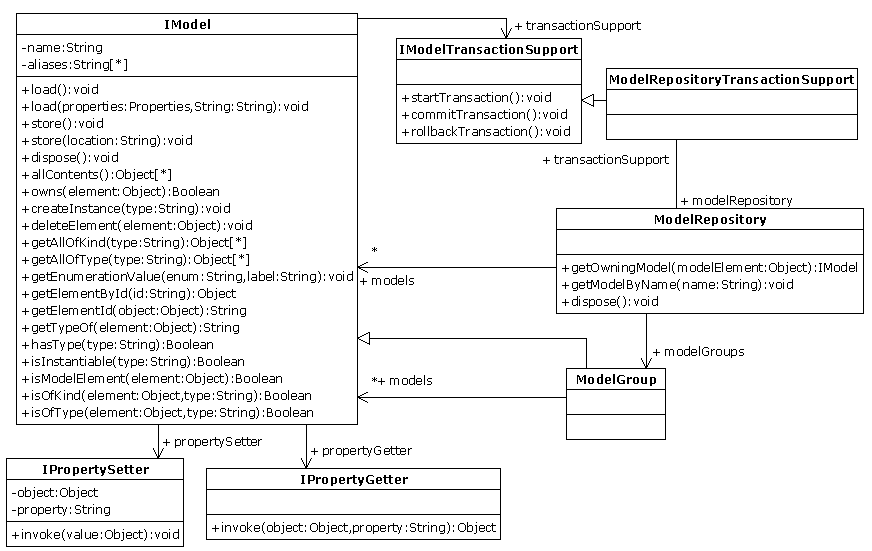
\includegraphics{images/EMC.png}
	\caption{Overview of the Epsilon Model Connectivity layer}
	\label{fig:EMC}
\end{figure}

\end{landscape}

To abstract away from diverse model representations and APIs provided by different modelling technologies, EMC defines the \emph{IModel} interface. \emph{IModel} provides a number of methods that enable querying and modifying the model elements it contains at a higher level of abstraction. To enable languages and tools that build atop EMC to manage multiple models simultaneously, the \emph{ModelRepository} class acts as a container that offers fa\c{c}ade services. The following sections discuss these two core concepts in detail.

\section{The IModel interface}

Each model specifies a name which must be unique in the context of the model repository in which it is contained. Also, it defines a number of aliases; that is non-unique alternate names; via which it can be accessed. The interface also defines the following services.

\section{Loading and Persistence}

The \emph{load()} and \emph{load(properties : Properties)} methods enable extenders to specify in a uniform way how a model is loaded into memory from the physical location in which it resides. Similarly, the \emph{store()} and \emph{store(location : String)} methods are used to define how the model can be persisted from memory to a permanent storage location.

\section{Type-related Services}

The majority of metamodelling architectures support inheritance between meta-classes and therefore two types of type-conformance relationships generally appear between model elements and types. The \emph{type-of} relationship appears when a model element is an instance of the type and the \emph{kind-of} relationship appears when the model element is an instance of the type or any of its sub-types. Under this definition, the \emph{getAllOfType( type : String )} and the \emph{getAllOfKind( type : String )} operations return all the elements in the model that have a type-of and a kind-of relationship with the type in question respectively.

Similarly, the \emph{isTypeOf( element : Object, type : String )} and \emph{isKindOf( element : Object, type : String)} return whether the element in question has a type-of or a kind-of relationship with the type respectively. The \emph{getTypeOf( element : Object )} method returns the fully-qualified name of the type an element conforms to.

The \emph{hasType( type : String )} method returns true if the model supports a type with the specified name. To support technologies that enable users to define abstract (non-instantiable) types, the \emph{isInstantiable( type : String )} method returns if instances of the type can be created.

\section{Ownership}

The \emph{allContents()} method returns all the elements that the model contains and the \emph{owns( element : Object )} method returns true if the element under question belongs to the model.

\section{Creation, Deletion and Modifications}
\label{sec:Design.EMC.CRUD}

Model elements are created and deleted using the \emph{createInstance( type : String )} and \emph{deleteElement( element : Object )} methods respectively.

To retrieve and set the values of properties of its model elements, \emph{IModel} uses its associated \emph{propertyGetter} (\emph{IPropertyGetter}) and \emph{propertySetter} (\emph{IPropertySetter}) respectively. Technology-specific implementations of those two interfaces are responsible for accessing and modifying the value of a property of a model element through their \emph{invoke( element : Object, property : String)} and \emph{invoke( value : Object )} respectively.

\section{The IModelTransactionSupport interface}
\label{sec:EMC.ModelTransactionSupport}
In its \emph{transactionSupport} property, a model can optionally (if the target modelling technology supports transactions) specify an instance of an implementation of the \emph{IModelTransactionSupport} interface. The interface provides transaction-related services for the specific modelling technology. The interface provides the \emph{startTransaction()}, \emph{commitTransaction()} and \emph{rollbackTransaction()} methods that start a new transaction, commit and roll back the current transaction respectively.

\section{The ModelRepository class}

A model repository acts as a container for a set of models that need to be managed in the context of a task or a set of tasks. Apart from a reference to the models it contains, \emph{ModelRepository} also provides the following fa\c{c}ade functionality.

The \emph{getOwningModel( element : Object )} method returns the model that owns a particular element. The \emph{transactionSupport} property specifies an instance of the \emph{ModelRepositoryTransactionSupport} class which is responsible for aggregate management of transactions by delegating calls to its \emph{startTransaction()}, \emph{commitTransaction()} and \emph{abortTransaction()} methods, to the respective methods of instances of \emph{IModelTransactionSupport} associated with models contained in the repository.

\section{The ModelGroup class}

A \emph{ModelGroup} is a group of models that have a common alias. \emph{ModelGroups} are calculated dynamically by the model repository based on common model aliases. That is, if two or more models share a common alias, the repository forms a new model group. Since \emph{ModelGroup} implements the \emph{IModel} interface, clients can use all the methods of \emph{IModel} to perform aggregate operations on multiple models, such as collecting the contents of more than one models. An exception to that is the \emph{createInstance( type : String )} method which cannot be defined for a group of models as it cannot be determined in which model of the group the newly created element should belong.

\section{Assumptions about the underlying modelling technologies}

The discussion provided above has demonstrated that EMC makes only minimal assumptions about the structure and the organization of the underlying modelling technologies. Thus, it intentionally refrains from defining classes for concepts such as \emph{model element}, \emph{type} and \emph{metamodel}. By contrast, it employs a lightweight approach that uses primitive strings for type names and objects of the target implementation platforms as  model elements. There are two reasons for this decision.

The primary reason is that by minimizing the assumptions about the underlying technologies EMC becomes more resistant to future changes of the implementations of the current technologies and can also embrace new technologies without changes.

Another reason is that if a heavy-weight approach was used, extending the platform with support for a new modelling technology would involve providing wrapping objects for the native objects which represent model elements and types in the specific modelling technology. Experiments in the early phases of the design of EMC demonstrated that such a heavy-weight approach significantly increases the amount of memory required to represent the models in memory, degrades performance and provides little benefits in reward\footnote{Recent developments in the context of the ATL transformation language have also demonstrated significant performance gains delivered by using native model element representations. Relevant benchmarks can be found \url{http://wiki.eclipse.org/ATL_VM_Testing}}.


%!TEX root = ./EpsilonBook.tex

\chapter{The Epsilon Object Language (EOL)}
\label{sec:Design.EOL}

The primary aim of EOL is to provide a reusable set of common model management facilities, atop which task-specific languages can be implemented. However, EOL can also be used as a general-purpose standalone model management language for automating tasks that do not fall into the patterns targeted by task-specific languages. This section presents the syntax and semantics of the language using a combination of abstract syntax diagrams, concrete syntax examples and informal discussion.

\section{Module Organization}
\label{sec:Design.EOL.Syntax}
\label{sec:Design.EOL.ModuleStucture}

In this section the syntax of EOL is presented in a top-down manner. As displayed in Figure \ref{fig:EOL.Module}, EOL programs are organized in \emph{modules}. Each module defines a \emph{body} and a number of \emph{operations}. The body is a block of statements that are evaluated when the module is executed\footnote{Although the EOL parser permits loose statements (e.g. not contained in operations) between/after operations, these are ignored at runtime.}. Each operation defines the kind of objects on which it is applicable (\emph{context}), a \emph{name}, a set of \emph{parameters} and optionally a \emph{return type}. Modules can also import other modules using \emph{import} statements and access their operations, as shown in Listing~\ref{lst:ExampleImports}.

\begin{sidewaysfigure}
  \centering
  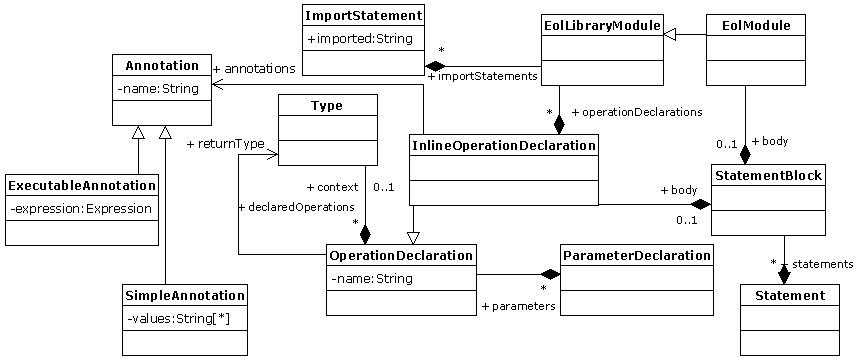
\includegraphics[width=\textwidth,height=\textheight,keepaspectratio]{images/EOLModule.png}
  \caption{EOL Module Structure}
  \label{fig:EOL.Module}
\end{sidewaysfigure}

\begin{lstlisting}[float, caption={Example of two related EOL modules}, label=lst:ExampleImports, language=EOL]
// file imported.eol
operation hello() {
  'Hello world!'.println();
}

// file importer.eol
// We can use relative/absolute paths or platform:/ URIs
import "imported.eol";

hello(); // main body

// ... more operations could be placed here ...
\end{lstlisting}

\section{User-Defined Operations}
\label{sec:Design.EOL.Operations}

In typical object oriented languages such as Java and C++, operations are defined inside classes and can be invoked on instances of those classes. EOL on the other hand is not object-oriented in the sense that it does not define classes itself, but nevertheless needs to manage objects of types defined externally to it (e.g. in metamodels). By defining the context-type of an operation explicitly, the operation can be called on instances of the type as if it was natively defined by the type. Alternatively, context-less operations could be defined; however the adopted technique significantly improves readability of the concrete syntax.

For example, consider the code excerpts displayed in Listings \ref{lst:OperationsContext} and \ref{lst:OperationsNoContext}. In Listing \ref{lst:OperationsContext}, the operations \emph{add1} and \emph{add2} are defined in the context of the built-in \emph{Integer} type, which is specified before their names. Therefore, they can be invoked in line 1 using the \emph{1.add1().add2()} expression: the context (the integer \emph{1}) will be assigned to the special variable \emph{self}. On the other hand, in Listing \ref{lst:OperationsNoContext} where no context is defined, they have to be invoked in a nested manner which follows an in-to-out direction instead of the left to right direction used by the former excerpt. As complex model queries often involve invoking multiple properties and operations, this technique is particularly beneficial to the overall readability of the code.

\begin{lstlisting}[float=tbp, caption={Context-defining EOL operations}, label=lst:OperationsContext, language=EOL]
1.add1().add2().println();

operation Integer add1() : Integer {
	return self + 1;
}

operation Integer add2() : Integer {
	return self + 2;
}
\end{lstlisting}

\begin{lstlisting}[float=tbp, caption={Context-less EOL operations}, label=lst:OperationsNoContext, language=EOL]
add2(add1(1)).println();

operation add1(base : Integer) : Integer {
	return base + 1;
}

operation add2(base : Integer) : Integer {
	return base + 2;
}
\end{lstlisting}

EOL supports polymorphic operations using a runtime dispatch mechanism. Multiple operations with the same name and parameters can be defined, each defining a distinct context type. For example, in Listing \ref{lst:Polymorphism}, the statement in line 1 invokes the test operation defined in line 4, while the statement in line 2 invokes the test operation defined in line 8.

\begin{lstlisting}[float=tbp, caption=Demonstration of polymorphism in EOL, label=lst:Polymorphism, numbers=left, language=EOL]
"1".test();
1.test();

operation String test() {
	(self + " is a string").println();
}

operation Integer test() {
	(self + "is an integer").println();
}

\end{lstlisting}

\subsection{Annotations}
\label{sec:Design.EOL.Annotations}
EOL supports two types of annotations: simple and executable. A simple annotation specifies a name and a set of String values while an executable annotation specifies a name and an expression. The concrete syntaxes of simple and executable annotations are displayed in Listings \ref{lst:SimpleAnnotations} and \ref{lst:ExecutableAnnotations} respectively. Several examples for simple annotations are shown in Listing~\ref{lst:SimpleAnnotationsExamples}. Examples for executable annotations will be given in the following sections.

\begin{lstlisting}[float=tbp, caption=Concrete syntax of simple annotations, label=lst:SimpleAnnotations, language=EOL, escapechar=!]
!\textbf{@}!name value(,value)*
\end{lstlisting}

\begin{lstlisting}[float=tbp, caption=Concrete syntax of executable annotations, label=lst:ExecutableAnnotations, language=EOL, escapechar=!]
!\textbf{\$}!name expression
\end{lstlisting}

\begin{lstlisting}[float=tbp, caption=Examples of simple annotations, label=lst:SimpleAnnotationsExamples, language=EOL, escapechar=!]
!\textbf{@}!colors red
!\textbf{@}!colors red, blue
!\textbf{@}!colors red, blue, green
\end{lstlisting}

In stand-alone EOL, annotations are supported only in the context of operations, however as discussed in the sequel, task-specific languages also make use of annotations in their constructs, each with task-specific semantics. EOL operations support three particular annotations: the \emph{pre} and \emph{post} executable annotations for specifying pre and post-conditions, and the \emph{cached} simple annotation, which are discussed below.

\subsection{Pre/post conditions in user-defined operations}
\label{sec:prep-cond-user}

A number of \emph{pre} and \emph{post} executable annotations can be attached to EOL operations to specify the pre- and post-conditions of the operation. When an operation is invoked, before its body is evaluated, the expressions of the \emph{pre} annotations are evaluated. If all of them return \emph{true}, the body of the operation is processed, otherwise, an error is raised. Similarly, once the body of the operation has been executed, the expressions of the \emph{post} annotations of the operation are executed to ensure that the operation has had the desired effects. \emph{Pre} and \emph{post} annotations can access all the variables in the parent scope, as well as the parameters of the operation and the object on which the operation is invoked (through the \emph{self} variable). Moreover, in \emph{post} annotations, the returned value of the operation is accessible through the built-in \emph{\_result} variable. An example of using pre and post conditions in EOL appears in Listing \ref{lst:PrePostConditionsExample}.

\begin{lstlisting}[float=tbp, caption=Example of pre- and post-conditions in an EOL operation, label=lst:PrePostConditionsExample, language=EOL]
1.add(2); /*@\label{line:ConditionsOK}@*/
1.add(-1); /*@\label{line:PreConditionFails}@*/

$pre i > 0 /*@\label{line:PreCondition}@*/
$post _result > self /*@\label{line:PostCondition}@*/
operation Integer add(i : Integer) : Integer {
	return self + i;
}
\end{lstlisting}

In line \ref{line:PreCondition} the \emph{add} operation defines a pre-condition stating that the parameter \emph{i} must be a positive number. In line \ref{line:PostCondition}, the operation defines that result of the operation (\emph{\_result}) must be greater than the number on which it was invoked (\emph{self}). Thus, when executed in the context of the statement in line \ref{line:ConditionsOK} the operation succeeds, while when executed in the context of the statement in line \ref{line:PreConditionFails}, the pre-condition is not satisfied and an error is raised. 

\subsection{Operation Result Caching}
\label{sec:EolCaching}

EOL supports caching the results of parameter-less operations using the \emph{@cached} simple annotation. In the following example, the Fibonacci number of a given Integer is calculated using the \emph{fibonacci} recursive operation displayed in Listing \ref{lst:Fibonacci}. Since the \emph{fibonacci} operation is declared as \emph{cached}, it is only executed once for each distinct Integer and subsequent calls on the same target return the cached result. Therefore, when invoked in line \ref{line:FibonnaciCall}, the body of the operation is called 16 times. By contrast, if no \emph{@cached} annotation was specified, the body of the operation would be called recursively 1973 times. This feature is particularly useful for performing queries on large models and caching their results without needing to introduce explicit variables that store the cached results.

Note that the cached result is not copied before it is returned, this has some implecations for returned lists of objects. For example, if a returned Set is modified, next time this modfied Set is returned instead of the original Set. If the Set needs to be modfied, first copy its contents into a new local Set.

\begin{lstlisting}[float=tbp, caption=Calculating the Fibonacci number using a cached operation, label=lst:Fibonacci, language=EOL]
15.fibonacci().println(); /*@\label{line:FibonnaciCall}@*/

@cached
operation Integer fibonacci() : Integer {
	if (self = 1 or self = 0) {
		return 1;
	}
	else {
		return (self-1).fibonacci() + (self-2).fibonacci();
	}
}
\end{lstlisting}

\section{Types}
\label{sec:eol_types}

As is the case for most programming languages, EOL defines a built-in system of types, illustrated in Figure \ref{fig:EOLTypes}. The \emph{Any} type, inspired by the \emph{OclAny} type of OCL, is the basis of all types in EOL including Collection types. The operations supported by instances of the Any type are outlined in Table \ref{tab:AnyOperations}\footnote{Parameters within square braces [ ] are optional}.

\begin{figure}[t]
  \centering
  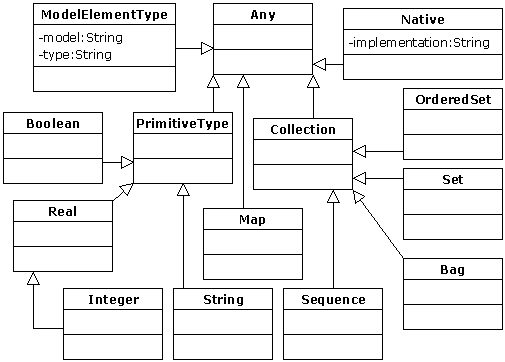
\includegraphics{images/EOLTypes.png}
  \caption{Overview of the type system of EOL}
  \label{fig:EOLTypes}
\end{figure}

\clearpage

\begin{longtabu} {|p{6.5cm}|X|}
			
			\caption{Operations of type Any}
			\label{tab:AnyOperations}\\
			
			\hline
							
			\textbf{Signature} & \textbf{Description} \\\hline

			isDefined() : Boolean & Returns true if the object is defined and false otherwise \\\hline
			
			isUndefined() : Boolean & Returns true if the object is undefined and false otherwise \\\hline
			
			ifUndefined(alt : Any) : Any & If the object is undefined, it returns alt else it returns the object \\\hline
			
			isTypeOf(type : Type) : Boolean & Returns true if the object is of the given type and false otherwise \\\hline
			
			isKindOf(type : Type) : Boolean & Returns true if the object is of the given type or one of its subtypes and false otherwise \\\hline
			
			type() : Type & Returns the type of the object. The EOL type system is illustrated in Figure \ref{fig:EOLTypes} \\\hline

                        owningModel() : Model & Returns the model that contains this object or an undefined value otherwise \\\hline

                        hasProperty(name : String) : Boolean & Returns true if the object has a property with the specified name or false otherwise \\\hline
                        
			asString() : String & Returns a string representation of the object \\\hline
			
			asInteger() : Integer & Returns an Integer based on the string representation of the object. If the string representation is not of an acceptable format, an error is raised \\\hline
			
			asReal() : Real & Returns a Real based on the string representation of the object. If the string representation is not of an acceptable format, an error is raised \\\hline
			
			asBoolean() : Boolean & Returns a Boolean based on the string representation of the object. If the string representation is not of an acceptable format, an error is raised \\\hline
			
			asBag() : Bag & Returns a new Bag containing the object \\\hline
			
			asSequence() : Sequence & Returns a new Sequence containing the object \\\hline
			
			asSet() : Set & Returns a new Set containing the object \\\hline
			
			asOrderedSet() : OrderedSet & Returns a new OrderedSet containing the object \\\hline
			
			print([prefix : String]) : Any & Prints a string representation of the object on which it is invoked to the regular output stream, prefixed with the optional \emph{prefix} string and returns the object on which it was invoked. In this way, the \emph{print} operation can be used for debugging purposes in a non-invasive manner\\\hline
			
			println([prefix : String]) : Any & Has the same effects as the \emph{print} operation but also produces a new line in the output stream. \\\hline

			err([prefix : String]) : Any & Prints a string representation of the object on which it is invoked to the error stream prefixed with the optional \emph{prefix} string and returns the object on which it was invoked. In this way, the \emph{print} operation can be used for debugging purposes in a non-invasive manner\\\hline
			
			errln([prefix : String]) : Any & Has the same effects as the \emph{err} operation but also produces a new line in the output stream. \\\hline
			
			format([pattern : String]) : String & Uses the provided pattern to form a String representation of the object on which the method is invoked. The pattern argument must conform to the format string syntax defined by Java\footnote{\url{http://download.oracle.com/javase/6/docs/api/java/util/Formatter.html\#syntax}}. \\\hline

\end{longtabu}

\subsection{Primitive Types} 

EOL provides four primitive types: String, Integer, Real and Boolean. The String type represents finite sequences of characters and supports the following operations which can be invoked on its instances.

\begin{longtabu} {|p{6.5cm}|X|}
			
			\caption{Operations of type String}
			\label{tab:StringOperations}\\
			
			\hline 
							
			\textbf{Signature} & \textbf{Description} \\\hline
			
			charAt(index : Integer) : String & Returns the character in the specified index\\\hline
			
			concat(str : String) : String & Returns a concatenated form of the string with the \emph{str} parameter\\\hline

			length() : Integer & Returns the number of characters in the string \\\hline
						
			toLowerCase() : String & Returns a new string where all the characters have been converted to lower case\\\hline
			
			firstToLowerCase() : String & Returns a new string the first character of which has been converted to lower case \\\hline
			
			toUpperCase() : String & Returns a new string where all the characters have been converted to upper case\\\hline
			
			firstToUpperCase() : String & Returns a new string, the first character of which has been converted to upper case \\\hline
			
			isSubstringOf(str : String) : Boolean & Returns true iff the string the operation is invoked on is a substring of \emph{str} \\\hline
			
			matches(reg : String) : Boolean & Returns true if there are occurrences of the regular expression \emph{reg} in the string\\\hline
			
			replace(source : String, target : String) : String & Returns a new string in which all instances of \emph{source} have been replaced with instances of \emph{target}\\\hline 
			
			split(reg : String) : Sequence(String) & Splits the string using as a delimiter the provided regular expression, \emph{reg}, and returns a sequence containing the parts\\\hline
			
			startsWith(str : String) : Boolean & Returns true iff the string starts with \emph{str}\\\hline
			
			endsWith(str : String) : Boolean & Returns true iff the string ends with \emph{str}\\\hline

			isInteger() : Boolean & Returns true iff the string is an integer\\\hline
			
			isReal() : Boolean & Returns true iff the string is a real number\\\hline
						
			toCharSequence() : Sequence(String) & Returns a sequence containing all the characters of the string\\\hline
			
			substring(index : Integer) : String & Returns a sub-string of the string starting from the specified \emph{index} and extending to the end of the original string\\\hline
			
			substring(startIndex : Integer, endIndex : Integer) : String & Returns a sub-string of the string starting from the specified \emph{startIndex} and ending at \emph{endIndex} \\\hline
			
			pad(length : Integer, padding : String, right : Boolean) : String & Pads the string up to the specified length with specified padding (e.g. "foo".pad(5, "*", true) returns "foo**") \\\hline
			
			trim() : String & Returns a trimmed copy of the string \\\hline			
			
\end{longtabu}

The Real type represents real numbers and provides the following operations.

\begin{longtabu} {|p{6.5cm}|X|}
			
			\caption{Operations of type Real}
			\label{tab:RealOperations}\\
			
			\hline
			
			\textbf{Signature} & \textbf{Description} \\\hline

			ceiling() : Integer & Returns the nearest Integer that is larger than the real\\\hline
			
			floor() : Integer & Returns the nearest Integer that is greater than the real\\\hline
			
			round() : Integer & Rounds the real to the nearest Integer\\\hline
			
			pow(exponent : Real) : Real & Returns the real to the power of exponent \\\hline
			
			log() : Real & Returns the natural logarithm of the real \\\hline
			
			log10() : Real & Returns the 10-based logarithm of the real \\\hline 
			
			abs() : Real & Returns the absolute value of the real \\\hline
			
			max(other : Real) : Real & Returns the maximum of the two reals \\\hline
			
			min(other : Real) : Real & Returns the minimum of the two reals \\\hline
			
\end{longtabu}

The Integer type represents natural numbers and negatives and extends the Real primitive type. It also defines the following operations:

\begin{longtabu} {|p{6.5cm}|X|}
			
			\caption{Operations of type Integer}
			\label{tab:IntegerOperations}\\
			
			\hline
							
			\textbf{Signature} & \textbf{Description} \\\hline

			to(other : Integer) : Sequence(Integer) & Returns a sequence of integers (e.g. 1.to(5) returns Sequence\{1,2,3,4,5\})\\\hline
			
			iota(end : Integer, step : Integer) : Sequence(Integer) & Returns a sequence of integers up to \emph{end} using the specified step (e.g. 1.iota(10,2) returns Sequence\{1,3,5,7,9\})\\\hline
			
\end{longtabu}

Finally, the Boolean type represents true/false states and provides no additional operations to those provided by the base Any type.

\subsection{Collections and Maps} 
\label{sec:Design.EOL.Collections}

EOL provides four types of collections and a Map type. The Bag type represents non-unique, unordered collections, the Sequence type represents non-unique, ordered collections, the Set type represents unique and unordered collections and the OrderedSet represents unique and ordered collections.

All collection types inherit from the abstract Collection type. Apart from simple operations, EOL also supports first-order logic operations on collections. The following operations apply to all types of collections:

\begin{longtabu} {|p{6.5cm}|X|}
			
			\caption{Operations of type Collection}
			\label{tab:Collection Operations}\\
			
			\hline
							
			\textbf{Signature} & \textbf{Description} \\\hline

			add(item : Any) & Adds an item to the collection. If the collection is a set, addition of duplicate items has no effect \\\hline
			
			addAll(col : Collection) & Adds all the items of the \emph{col} argument to the collection. If the collection is a set, it only adds items that do not already exist in the collection\\\hline
		
			remove(item : Any) & Removes an \emph{item} from the collection \\\hline
			
			removeAll(col : Collection) & Removes all the items of \emph{col} from the collection \\\hline
			
			clear() & Empties the collection \\\hline
			
			includes(item : Any) : Boolean & Returns true if the collection includes the \emph{item} \\\hline
			
			excludes(item : Any) : Boolean & Returns true if the collection excludes the \emph{item} \\\hline
			
			includesAll(col : Collection) : Boolean & Returns true if the collection includes all the items of collection \emph{col} \\\hline
			
			excludesAll(col : Collection) : Boolean & Returns true if the collection excludes all the items of collection col \\\hline
			
			including(item : Any) : Collection & Returns a new collection that also contains the \emph{item} -- unlike the add() operation that adds the \emph{item} to the collection itself  \\\hline
			
			excluding(item : Any) : Collection & Returns a new collection that excludes the item -- unlike the remove() operation that removes the \emph{item} from the collection itself\\\hline
			
			includingAll(col : Collection) : Collection & Returns a new collection that is a union of the two collections. The type of the returned collection (i.e. Bag, Sequence, Set, OrderedSet) is same as the type of the collection on which the operation is invoked \\\hline
			
			excludingAll(col : Collection) : Collection & Returns a new collection that excludes all the elements of the col collection \\\hline
			
			flatten() : Collection & Recursively flattens all items that are of collection type and returns a new collection where no item is a collection itself \\\hline
			
			count(item : Any) : Integer & Returns the number of times the item exists in the collection \\\hline
			
			size() : Integer & Returns the number of items the collection contains \\\hline

			sum() : Real & Returns the sum of all reals/integers in the collection\\\hline

			product() : Real & Returns the product of all reals/integers in the collection\\\hline
			
			isEmpty() : Boolean & Returns true if the collection does not contain any elements and false otherwise \\\hline
	
			random() : Any & Returns a random item from the collection \\\hline
			
			clone() : Collection & Returns a new collection of the same type containing the same items with the original collection \\\hline
			
			concat() : String & Returns the string created by converting each element of the collection to a string \\\hline
			
			concat(separator : String) : String & Returns the string created by converting each element of the collection to a string, using the given argument as a separator \\\hline
\end{longtabu}

The following operations apply to ordered collection types (i.e. Sequence and OrderedSet):

\begin{longtabu} {|p{6.5cm}|X|}
			
			\caption{Operations of types Sequence and OrderedSet}
			\label{tab:SortedOperations}\\
			
			\hline
							
			\textbf{Signature} & \textbf{Description} \\\hline

			first() : Any & Returns the first item of the collection  \\\hline

			second() : Any & Returns the second item of the collection  \\\hline

			third() : Any & Returns the third item of the collection  \\\hline

			fourth() : Any & Returns the fourth item of the collection  \\\hline
				
			last() : Any & Returns the last item of the collection  \\\hline
	
			at(index : Integer) : Any & Returns the item of the collection at the specified index \\\hline
			
			removeAt(index : Integer) : Any & Removes and returns the item at the specified index. \\\hline
			
			indexOf(item : Any) : Integer & Returns the index of the item in the collection or -1 if it does not exist \\\hline

			invert() : Collection & Returns an inverted copy of the collection\\\hline
						
\end{longtabu}

Also, EOL collections support the following first-order operations:

\begin{longtabu} {|p{6.5cm}|X|}
			
			\caption{First-order logic operations on Collections}
			\label{tab:FirstOrderOperations}\\
			
			\hline
							
			\textbf{Signature} & \textbf{Description} \\\hline

			select(iterator : Type $|$ condition) : Collection & Returns a sub-collection containing only items of the specified type that satisfy the condition \\\hline 

			selectOne(iterator : Type $|$ condition) : Any & Returns the first element that satisfies the condition \\\hline
			
			reject(iterator : Type $|$ condition) : Collection & Returns a sub-collection containing only items of the specified type that do not satisfy the condition \\\hline
			
			collect(iterator : Type $|$ expression) : Collection &  Returns a collection containing the results of evaluating the expression on each item of the collection that is of the specified type \\\hline

                        closure(iterator : Type $|$ expression) : Collection & Returns a collection containing the results of evaluating the transitive closure of the results produced by the expression on each item of the collection that is of the specified type \\\hline

                        aggregate(iterator : Type $|$ keyExpression, valueExpression) : Map & Returns a map containing key-value pairs produced by evaluating the key and value expressions on each item of the collection that is of the specified type \\\hline

			one(iterator : Type $|$ condition) : Boolean & Returns true if there exists exactly one item in the collection that satisfies the condition \\\hline

			exists(iterator : Type $|$ condition) : Boolean & Returns true if there exists at least one item in the collection that satisfies the condition \\\hline
			
			forAll(iterator : Type $|$ condition) : Boolean & Returns true if all items in the collection satisfy the condition \\\hline
			
			%iterate(iterator : IteratorType ; result : ResultType = initialValue $|$ expression) : ResultType & Iterates all the items of the collection that conform to the IteratorType and incrementally calculates the value of the result variable which it finally returns \\\hline
			
			sortBy(iterator: Type $|$ expression) : Collection & Returns a copy of the collection sorted by the results of evaluating the expression on each item of the collection that conforms to the iterator type \\\hline

\end{longtabu}

The Map type represents an array of key-value pairs in which the keys are unique. The type provides the following operations.

\begin{longtabu} {|p{6.5cm}|X|}
			
			\caption{Operations of type Map}
			\label{tab:MapOperations}\\
			
			\hline
			
			\textbf{Signature} & \textbf{Description} \\\hline

			put(key : Any, value : Any) & Adds the key-value pair to the map. If the map already contains the same key, the value is overwritten\\\hline
				
			get(key : Any) : Any & Returns the value for the specified keys\\\hline
	
			containsKey(key : Any) : Boolean & Returns true if the map contains the specified key\\\hline
	
			keySet() : Set & Returns the keys of the map\\\hline
			
			values() : Bag & Returns the values of the map\\\hline
			
			clear() & Clears the map\\\hline
			
\end{longtabu}

\subsection{Native Types}

As discussed earlier, while the purpose of EOL is to provide significant expressive power to enable users to manage models at a high level of abstraction, it is not intended to be a general-purpose programming language. Therefore, there may be cases where users need to implement some functionality that is either not efficiently supported by the EOL runtime (e.g. complex mathematical computations) or that EOL does not support at all (e.g. developing user interfaces, accessing databases). To overcome this problem, EOL enables users to create objects of the underlying programming environment by using \emph{native} types. A native type specifies an $implementation$ property that indicates the unique identifier for an underlying platform type. For instance, in a Java implementation of EOL the user can instantiate and use a Java class via its class identifier. Thus, in Listing \ref{lst:Native} the EOL excerpt creates a Java window (Swing JFrame) and uses its methods to change its title and dimensions and make it visible.

\begin{lstlisting}[float=tbp, caption=Demonstration of NativeType in EOL, label=lst:Native, language=EOL]
var frame = new Native("javax.swing.JFrame");
frame.title = "Opened with EOL";
frame.setBounds(100,100,300,200);
frame.visible = true;
\end{lstlisting}

To pass arguments to the constructor of a native type, a parameter list must be added, such as that in Listing~\ref{lst:Native-params}.

\begin{lstlisting}[float=tbp, caption=Demonstration of NativeType in EOL, label=lst:Native-params, numbers=left, language=EOL]
var file = new Native("java.io.File")("myfile.txt");
file.absolutePath.println();
\end{lstlisting}

\subsection{Model Element Types}

A model element type represents a meta-level classifier. As discussed in Section \ref{sec:Design.EMC}, Epsilon intentionally refrains from defining more details about the meaning of a model element type to be able to support diverse modelling technologies where a type has different semantics. For instance a MOF class, an XSD complex type and a Java class can all be regarded as model element types according to the implementation of the underlying modelling framework.

In case of multiple models, as well as the name of the type, the name of the model is also required to resolve a particular type since different models may contain elements of homonymous but different model element types. In case a model defines more than one type with the same name (e.g. in different packages), a fully qualified type name must be provided.

In terms of concrete syntax, inspired by ATL, the ! character is used to separate the name of the type from the name of the model it is defined in. For instance $Ma!A$ represents the type $A$ of model $Ma$. Also, to support modelling technologies that provide hierarchical grouping of types (e.g. using packages) the :: notation is used to separate between packages and classes.  A model element type supports the following operations:

\begin{longtabu} {|p{6.5cm}|X|}
			
			\caption{Operations of Model Element Types}
			\label{tab:ModelElementTypesOperations}\\
			
			\hline
			
			\textbf{Signature} & \textbf{Description} \\\hline
			
			allOfType() : Set & Returns all the elements in the model that are instances of the type \\\hline
			
			allOfKind() : Set & Returns all the elements in the model that are instances either of the type itself or of one of its subtypes  \\\hline

			allInstances() : Set & Alias for allOfKind() (for compatibility with OCL) \\\hline
						
			all() : Set & Alias for allOfKind() (for syntax-compactness purposes) \\\hline
			
			isInstantiable() : Boolean & Returns true if the type is instantiable (i.e. non-abstract)  \\\hline
			
			createInstance() : Any & Creates an instance of the type in the model \\\hline
			
\end{longtabu}

As an example of the concrete syntax, Listing \ref{lst:ModelElementTypes} retrieves all the instances of the Class type (including instances of its subtypes) defined in the Core package of the UML 1.4 metamodel that are contained in the model named UML14.

\begin{lstlisting}[float=tbp, caption=Demonstration of the concrete syntax for accessing model element types, label=lst:ModelElementTypes, language=EOL]
UML14!Core::Foundation::Class.allInstances();
\end{lstlisting}

\section{Expressions}

\subsection{Literal Values}

EOL provides special syntax constructs to create instances of each of the built-in types:

\begin{description}
\item[Integer] literals are defined by using one or more decimal
  digits (such as \emph{42} or \emph{999}). Optionally, long integers
  (with the same precision as a Java \emph{Long}) can be produced by
  adding a ``l'' suffix, such as \emph{42l}.

\item[Real] literals are defined by:
  \begin{itemize}
  \item Adding a decimal separator and non-empty fractional part to
    the integer part, such as \emph{42.0} or \emph{3.14}. Please note
    that \emph{.2} and \emph{2.} are \emph{not} valid literals.
  \item Adding a floating point suffix: ``f'' and ``F'' denote single
    precision, and ``d'' and ``D'' denote double precision. For
    example, \emph{2f} or \emph{3D}.
  \item Adding an exponent, such as \emph{2e+1} (equal to \emph{2e1})
    or \emph{2e-1}.
  \item Using any combination of the above options.
  \end{itemize}

\item[String] literals are sequences of characters delimited by single
  (\verb#'hi'#) or double (\verb#"hi"#) quotes. Quotes inside the
  string can be escaped by using a backslash, such as in \verb#'A\'s'#
  or \verb#"A\"s"#. Literal backslashes need to be escaped as well,
  such as in \verb#'A\\B'#. Special escape sequences are also
  provided: \verb#\n# for a newline, \verb#\t# for a horizontal tab
  and \verb#\r# for a carriage return, among others.

\item[Boolean] literals use the \emph{true} reserved keyword for the
  true Boolean value, and \emph{false} reserved keyword for the false
  Boolean value.

\item[Sequence] and most other collections (except \emph{Map}s) also
  have literals. Their format is \emph{T \{e\}}, where \emph{T} is the
  name of the type and \emph{e} are zero or more elements, separated
  by commas. For instance, \emph{Sequence \{\}} is the empty sequence,
  and \emph{Set \{1, 2, 3\}} is the set of numbers between 1 and 3.

\item[Map] literals are similar to the sequential collection literals,
  but their elements are of the form \emph{key = value}. For instance,
  \emph{Map \{'a' = 1, 'b' = 2\}} is a map which has two keys, ``a''
  and ``b'', which map to the integer values 1 and 2, respectively.

  Please note that, when defining an element such as \emph{1 = 2 = 3},
  the key would be \emph{1} and the value would be the result of
  evaluating \emph{2 = 3} (false). If you would like to use the result
  of the expression \emph{1 = 2} as key, you will need to enclose it
  in parenthesis, such as in \emph{(1 = 2) = 3}.

\end{description}

\subsection{Feature Navigation}
\label{sec:Design.EOL.FeatureNavigation}
Since EOL needs to manage models defined using object oriented modelling technologies, it provides expressions to navigate properties and invoke simple and declarative operations on objects (as presented in Figure \ref{fig:EOLExpressions}). 

\begin{figure}
	\centering
		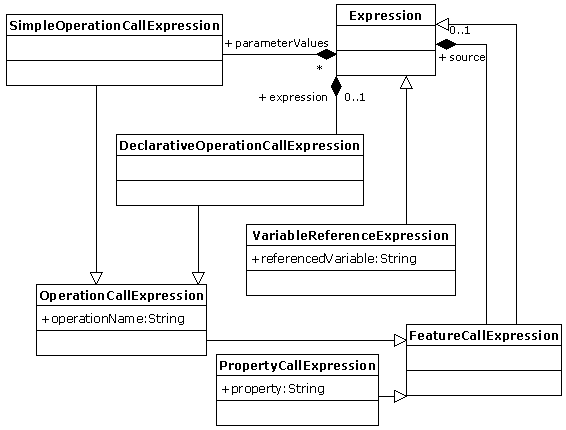
\includegraphics{images/EOLExpressions.png}
	\caption{Overview of the feature navigation EOL expressions}
	\label{fig:EOLExpressions}
\end{figure}

In terms of concrete syntax, `.' is used as a uniform operator to access a property of an object and to invoke an operation on it. The `$\rightarrow$' operator, which is used in OCL to invoke first-order logic operations on sets, has been also preserved for syntax compatibility reasons. In EOL, every operation can be invoked both using the `.' or the '$\rightarrow$' operators, with a slightly different semantics to enable overriding the built-in operations. If the `.' operator is used, precedence is given to the user-defined operations, otherwise precedence is given to the built-in operations. For instance, the Any type defines a println() method that prints the string representation of an object to the standard output stream. In Listing \ref{lst:Expressions}, the user has defined another parameterless println() operation in the context of Any. Therefore the call to println() in Line 1 will be dispatched to the user-defined println() operation defined in line 3. In its body the operation uses the `$\rightarrow$' operator to invoke the built-in println() operation (line 4).

\begin{lstlisting}[float=tbp, caption=Invoking operations using EOL, label=lst:Expressions, language=EOL]
"Something".println();

operation Any println() : Any {
	("Printing : " + self)->println();
}
\end{lstlisting}

\subsection{Arithmetical and Comparison Operators}

EOL provides common operators for performing arithmetical computations and comparisons illustrated in Tables \ref{tab:ArithmeticalOperators} and \ref{tab:ComparisonOperators} respectively.

%Figures \ref{fig:EOLArithmeticalOperators} and \ref{fig:EOLComparisonOperators} respectively.
%
%\begin{figure}
%	\centering
%		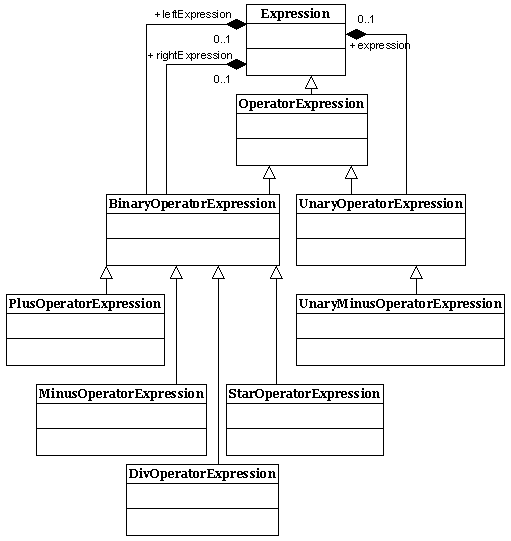
\includegraphics{images/EOLArithmeticalOperators}
%	\caption{Overview of the arithmetical EOL operator expressions}
%	\label{fig:EOLArithmeticalOperators}
%\end{figure}
%
%\begin{figure}
%	\centering
%		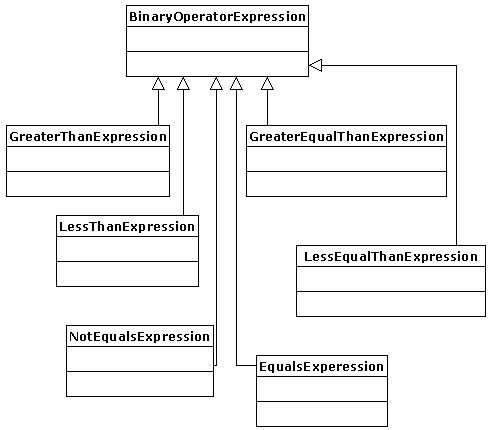
\includegraphics{images/EOLComparisonOperators}
%	\caption{Overview of the comparison EOL operator expressions}
%	\label{fig:EOLComparisonOperators}
%\end{figure}

\begin{longtabu} {|p{3.5cm}|X|}
			
			\caption{Arithmetical operators}
			\label{tab:ArithmeticalOperators}\\
			
			\hline
							
			\textbf{Operator} & \textbf{Description} \\\hline

				$+$ & Adds reals/integers and concatenates strings \\\hline
	
				$-$ & Subtracts reals/integers \\\hline
				
				$-$ (unary) & Returns the negative of a real/integer \\\hline
				
				$*$ & Multiplies reals/integers \\\hline
				
				$/$ & Divides reals/integers \\\hline
				
\end{longtabu}

\clearpage

\begin{longtabu} {|p{3.5cm}|X|}
			
			\caption{Comparison operators}
			\label{tab:ComparisonOperators}\\
			
			\hline
							
			\textbf{Operator} & \textbf{Description} \\\hline

			$=$ & Returns true if the left hand side equals the right hand side. In the case of primitive types (String, Boolean, Integer, Real) the operator compares the values; in the case of objects it returns true if the two expressions evaluate to the same object \\\hline
			
			$<>$ & Is the logical negation of the ($=$) operator \\\hline
				
			$>$ & For reals/integers returns true if the left hand side is greater than the right hand side number \\\hline
			
			$<$ & For reals/integers returns true if the left hand side is less than then right hand side number \\\hline
			
			$>=$ & For reals/integers returns true if the left hand side is greater or equal to the right hand side number \\\hline
			
			$<=$ & For reals/integers returns true if the left hand side is less or equal to then right hand side number \\\hline
		
\end{longtabu}

\subsection{Logical Operators}

EOL provides common operators for performing logical computations illustrated in Table \ref{tab:LogicalOperators}. Logical operations apply only to instances of the Boolean primitive type.

%\begin{figure}
%	\centering
%		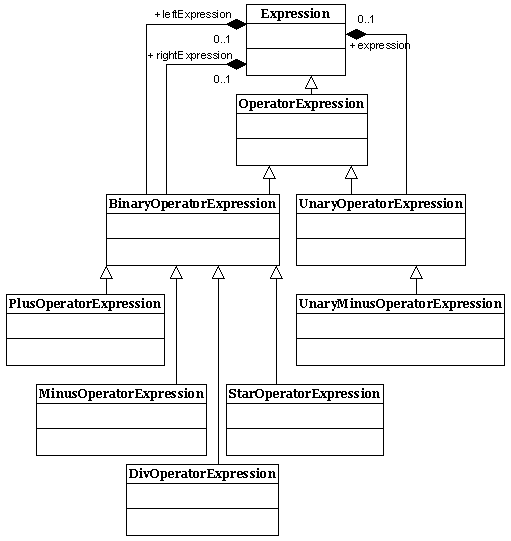
\includegraphics{images/EOLArithmeticalOperators}
%	\caption{Overview of the logical EOL operator expressions}
%	\label{fig:EOLLogicalOperators}
%\end{figure}

\begin{longtabu} {|p{3.5cm}|X|}
			
			\caption{Logical Operators}
			\label{tab:LogicalOperators}\\
			
			\hline
							
			\textbf{Operator} & \textbf{Description} \\\hline

			and & Returns the logical conjunction of the two expressions \\\hline
			
			or & Returns the logical disjunction of the two expressions \\\hline
			
			not & Returns the logical negation of the expression \\\hline
			
			implies & Returns the logical implication of the two expressions. Implication is calculated according to the truth table \ref{tab:ImpliesTruthTable} \\\hline
			
			xor & returns true if only one of the involved expressions evaluates to true  and false otherwise \\\hline
	
\end{longtabu}
	
\begin{longtable} {|l|l|l|} 
	
	\caption{Implies Truth Table}
	\label{tab:ImpliesTruthTable}\\
	
	\hline
		\textbf{Left} & \textbf{Right} & \textbf{Result} \\\hline
		true & true & true \\\hline
		true & false & false \\\hline
		false & true & true \\\hline
		false & false & true \\\hline			

\end{longtable}

\subsection{Enumerations}

EOL provides the \# operator for accessing enumeration literals. For example, the VisibilityEnum\#vk\_public expression returns the value of the literal \emph{vk\_public} of the \emph{VisibilityEnum} enumeration. For EMF metamodels, \emph{VisibilityEnum\#vk\_public.instance} can also be used.

\section{Statements}

\subsection{Variable Declaration Statement}

A variable declaration statement declares the name and (optionally) the type and initial value of a variable in an EOL program. If no type is explicitly declared, the variable is assumed to be of type Any. For variables of primitive type, declaration automatically creates an instance of the type with the default values presented in Table \ref{tab:DefaultValuesOfPrimitiveTypes}. For non-primitive types the user has to explicitly assign the value of the variable either by using the \emph{new} keyword or by providing an initial value expression. If neither is done the value of the variable is undefined. Variables in EOL are strongly-typed. Therefore a variable can only be assigned values that conform to its type (or a sub-type of it).

\begin{table}
  \centering
  \caption{Default values of primitive types}
  \label{tab:DefaultValuesOfPrimitiveTypes}
  \begin{tabular}{|l|l|}
    \hline
    \textbf{Type} & \textbf{Default value} \\\hline
    Integer       & 0                      \\\hline
    Boolean       & false                  \\\hline
    String        & ""                     \\\hline
    Real          & 0.0                    \\\hline
  \end{tabular}
\end{table}

\paragraph{Scope} The scope of variables in EOL is generally limited to the block of statements where they are defined, including any nested blocks. Nevertheless, as discussed in the sequel, there are cases in task-specific languages that build atop EOL where the scope of variables is expanded to other non-nested blocks as well. EOL also allows variable shadowing; that is to define a variable with the same name in a nested block that overrides a variable defined in an outer block. 

In Listing \ref{lst:Variables}, an example of declaring and using variables is provided. Line 1 defines a variable named \emph{i} of type \emph{Integer} and assigns it an initial value of \emph{5}. Line 2 defines a variable named \emph{c} of type \emph{Class} (from model Uml) and creates a new instance of the type in the model (by using the \emph{new} keyword). The commented out assignment statement of line 3 would raise a runtime error since it would attempt to assign a \emph{String} value to an \emph{Integer} variable. The condition of line 4 returns true since the \emph{c} variable has been initialized before. Line 5 defines a new variable also named \emph{i} that is of type \emph{String} and which overrides the \emph{Integer} variable declared in line 1. Therefore the assignment statement of line 6 is legitimate as it assigns a string value to a variable of type String. Finally, as the program has exited the scope of the \emph{if} statement, the assignment statement of line 7 is also legitimate as it refers to the \emph{i} variable defined in line 1.

\begin{lstlisting}[float=tbp, caption=Example illustrating declaration and use of variables, label=lst:Variables, language=EOL]
var i : Integer = 5;
var c : new Uml!Class;
//i = "somevalue";
if (c.isDefined()) {
	var i : String;
	i = "somevalue";
}
i = 3;
\end{lstlisting}

\subsection{Assignment Statement}

The assignment statement is used to update the values of variables and  properties of native objects and model elements.

\paragraph{Variable Assignment}

When the left hand side of an assignment statement is a variable, the value of the variable is updated to the object to which the right hand side evaluates to. If the type of the right hand side is not compatible (kind-of relationship) with the type of the variable, the assignment is illegal and a runtime error is raised. Assignment to objects of primitive types is performed by value while assignment to instances of non-primitive values is performed by reference. For example, in Listing \ref{lst:VariableAssignmentByReference}, in line 1 the value
of the a variable is set to a new Class in the Uml model. In line 2, a new untyped variable b is declared and its value is assigned to a. In line 3 the name of the class is updated to Customer and thus, line 4 prints Customer to the standard output stream. On the other hand, in Listing \ref{lst:VariableAssignmentByValue}, in line 1 the a String variable is declared. In line 2 an untyped variable b is declared. In line 3, the value of a is changed to Customer (which is an instance of the primitive \emph{String} type). This has no effect on b and thus line 4 prints an empty string to the standard output stream.

\begin{lstlisting}[float=tbp, caption=Assigning the value of a variable by reference, label=lst:VariableAssignmentByReference, language=EOL]
var a : new Uml!Class;
var b = a;
a.name = "Customer";
b.name.println();
\end{lstlisting}

\begin{lstlisting}[float=tbp, caption=Assigning the value of a variable by value, label=lst:VariableAssignmentByValue, language=EOL]
var a : String;
var b = a;
a = "Customer";
b.println();
\end{lstlisting}

\paragraph{Native Object Property Assignment}

When the left hand side of the assignment is a property of a native object, deciding on the legality and providing the semantics of the assignment is delegated to the execution engine. For example, in a Java-based execution engine, given that x is a native object, the statement \emph{x.y = a} may be interpreted as \emph{x.setY(a)} or if x is an instance of a map \emph{x.put(''y'',a)}. By contrast, in a C\# implementation, it can be interpreted as \emph{x.y = a} since
the language natively supports properties in classes.

\paragraph{Model Element Property Assignment}

When the left hand side of the assignment is a property of a model element, the model that owns the particular model element (accessible using the \emph{ModelRepository.getOwningModel() }operation) is responsible for implementing the semantics of the assignment using its associated \emph{propertyGetter} as discussed in Section \ref{sec:Design.EMC.CRUD}. For example, if x is a model element, the statement \emph{x.y = a} may be interpreted using the Java code of Listing \ref{lst:EmfModelElementPropertyAssignment} if x belongs to an EMF-based model or using the Java code of Listing \ref{lst:MdrModelElementPropertyAssignment} if it belongs to an MDR-based model.

\begin{lstlisting}[float=tbp, caption=Java code that assigns the value of a property of a model element that belongs to an EMF-based model, label=lst:EmfModelElementPropertyAssignment, language=Java]
EStructuralFeature feature = x.eClass().getEStructuralFeature("y");
x.eSet(feature, a);
\end{lstlisting}

\begin{lstlisting}[float=tbp, caption=Java code that assigns the value of a property of a model element that belongs to an MDR-based model, label=lst:MdrModelElementPropertyAssignment, language=Java]
StructuralFeature feature = findStructuralFeature(x.refClass(), "y");
x.refSetValue(feature, a);
\end{lstlisting}

\subsection{Special Assignment Statement}
\label{sec:Design.EOL.SpecialAssignmentStatement}
In task-specific languages, an assignment operator with task-specific semantics is often required. Therefore, EOL provides an additional assignment operator. In standalone EOL, the operator has the same semantics with the primary assignment operator discussed above, however task-specific languages can redefine its semantics to implement custom
assignment behaviour. For example, consider the simple model-to-model transformation of Listing \ref{lst:SpecialAssignmentStatement} where a simple object oriented model is transformed to a simple database model using an ETL (see Section \ref{sec:ETL}) transformation. The Class2Table rule transforms a Class of the OO model into
a Table in the DB model and sets the name of the table to be the same as the name of the class. Rule Atribute2Column transforms an Attribute from the OO model into a column in the DB model. Except for setting its name (line 12), it also needs to define that the column belongs to the table which corresponds to the class that defines the source attribute. The commented-out assignment statement of line 13 cannot
be used for this purpose since it would illegaly attempt to assign the owningTable feature of the column to a model element of an inappropriate type (OO!Class). However, the special assignment operator in the task-specific language implements the semantics discussed in Section \ref{sec:Design.ETL.SpecialAssignmentOperator}, and thus in line 14 it assigns to the owningTable feature not the class that owns the attribute but its corresponding table (calculated using the Class2Table rule) in the DB model. 

\begin{lstlisting}[float=tbp, caption=A simple model-to-model transformation
demonstrating the special assignment statement, label=lst:SpecialAssignmentStatement, language=ETL]
rule Class2Table
  transform c : OO!Class
  to t : DB!Table {
  
  t.name = c.name;
}

rule Attribute2Column
  transform a : OO!Attribute
  to c : DB!Column {
  
  c.name = a.name;
  //c.owningTable = c.owningClass;
  c.owningTable ::= c.owningClass;
}

\end{lstlisting}

\subsection{If Statement}

As in most programming languages, an if statement consists of a condition, a block of statements that is executed if the condition is satisfied and (optionally) a block of statements that is executed otherwise. As an example, in Listing \ref{lst:IfStatement}, if variable a holds a value that is greater than 0 the statement of line 3 is executed, otherwise the statement of line 5 is executed.

\begin{lstlisting}[float=h, caption=Example illustrating an if statement, label=lst:IfStatement, language=EOL]
if (a > 0) {
	"A is greater than 0".println();
}
else { "A is less equal than 0".println(); }
\end{lstlisting}

\subsection{Switch Statement}

A switch statement consists of an expression and a set of cases, and can be used to implement multi-brancing. Unlike Java/C, switch in EOL doesn't by default fall through to the next case after a successful one. Therefore, it is not necessary to add a \emph{break} statement after each case. To enable falling through to the next case you can use the \emph{continue} statement. Also, unlike Java/C, the switch expression can return anything (not only integers). As an example, when executed, the code in Listing \ref{lst:SwitchStatement1} prints 2 while the code in Listing \ref{lst:SwitchStatement2} prints 2,3,default.

\begin{lstlisting}[float=h, caption=Example illustrating a switch statement, label=lst:SwitchStatement1, language=EOL]
var i = "2";

switch (i) {
	case "1" : "1".println(); 
	case "2" : "2".println();
	case "3" : "3".println();
	default : "default".println(); 
}
\end{lstlisting}

\begin{lstlisting}[float=h, caption=Example illustrating falling through cases in a switch statement, label=lst:SwitchStatement2, language=EOL]
var i = "2";

switch (i) {
	case "1" : "1".println(); 
	case "2" : "2".println(); continue;
	case "3" : "3".println();
	default : "default".println(); 
}
\end{lstlisting}

\subsection{While Statement}
\label{sec:while-statement}

A while statement consists of a condition and a block of statements which are executed as long as the condition is satisfied. For example, in Listing \ref{lst:WhileStatement} the body of the while statement is executed 5 times printing the numbers 0 to 4 to the output console. Inside the body of a \emph{while} statement, the built-in read-only \emph{loopCount} integer variable holds the number of times the innermost loop has been executed so far (including the current iteration). Right after entering the loop for the first time and before running the first statement in its body, \emph{loopCount} is set to 1, and it is incremented after each following iteration.

\begin{lstlisting}[float=h, caption=Example of a while statement, label=lst:WhileStatement, numbers=left, language=EOL]
var i : Integer = 0;
while (i < 5) {
  // both lines print the same thing
  i.println();
  (loopCount - 1).println();
  // increment the counter
  i = i+1;
}
\end{lstlisting}

\subsection{For Statement}

In EOL, for statements are used to iterate the contents of collections. A for statement defines a typed iterator and an iterated collection as well as a block of statements that is executed for every item in the collection that has a kind-of relationship with the type defined by the iterator. As with the majority of programming languages, modifying a collection while iterating it raises a runtime error. To avoid this situation, users can use the clone() built-in operation of the Collection type discussed in \ref{sec:Design.EOL.Collections}. 

\begin{lstlisting}[float=h, caption=Example of a for statement, label=lst:ForStatement, language=EOL]
var col : Sequence = Sequence{"a", 1, 2, 2.5, "b"};
for (r : Real in col) {
	r.print();
	if (hasMore){",".print();}
}
\end{lstlisting}

Inside the body of a \emph{for} statement two built-in read-only variables are visible: the \emph{loopCount} integer variable (explained in Section~\ref{sec:while-statement}) and the \emph{hasMore} boolean variable. \emph{hasMore} is used to determine if there are more items if the collection for which the loop will be executed. For example, in Listing \ref{lst:ForStatement} the col heterogeneous Sequence is defined that contains two strings (a and b), two integers (1,2) and one real (2.5). The for loop of line 2 only iterates through the items of the collection that are of kind Real and therefore prints 1,2,2.5 to the standard output stream.

\begin{lstlisting}[float=h, caption=Example of a for statement, label=lst:TransactionStatement, language=EOL]
var system : System.allInstances.first();

for (i in Sequence {1..100}) {

	transaction {
		
		var failedProcessors : Set; 
		
		while (failedProcessors.size() < 10) {
			failedProcessors.add(system.processors.random());
		}
		
		for (processor in failedProcessors) {
			processor.failed = true;
			processor.moveTasksElsewhere();
		}
		
		system.evaluateAvailability();
		
		abort; /*@\label{line:Abort}@*/
	}
	
}
\end{lstlisting}

\begin{lstlisting}[float=h, caption=Calculating and printing the depth of each Tree, label=lst:NoExtendedProperties, language=EOL]
var depths = new Map; /*@\label{line:DeclareMap}@*/

for (n in Tree.allInstances.select(t|not t.parent.isDefined())) {
	n.setDepth(0);
}

for (n in Tree.allInstances) {
	(n.name + " " + depths.get(n)).println();
}

operation Tree setDepth(depth : Integer) {
	depths.put(self,depth); /*@\label{line:PutDepthInMap}@*/
	for (c in self.children) {
		c.setDepth(depth + 1);
	}
}
\end{lstlisting}

\subsection{Break, BreakAll and Continue Statements}

To exit from for and while loops on demand, EOL provides the break and breakAll statements. The break statement exits the innermost loop while the breakAll statement exits all outer loops as well. On the other hand, to skip a particular loop and proceed with the next one, EOL provides the continue statement. For example, the excerpt of Listing \ref{lst:BreakStatement}, prints \textit{2,1 3,1} to the standard output stream.

\begin{lstlisting}[float=h, caption=Example of the break\, breakAll and continue statements, label=lst:BreakStatement, language=EOL]
for (i in Sequence{1..3}) {
	if (i = 1) {continue;}
	for (j in Sequence{1..4}) {
		if (j = 2) {break;}
		if (j = 3) {breakAll;}
		(i + "," + j).println();
	}
}
\end{lstlisting}

\subsection{Throw Statement}
\label{sec:eol-throw}

EOL provides the throw statement for throwing a value as an \class{EolUserException} Java exception. This is especially useful when invoking EOL scripts from Java code: by catching and processing the exception, the Java code may be able to automatically handle the problem without requiring user input. Any value can be thrown, as shown in Listing~\ref{lst:ThrowStatement}, where we throw a number and a string.

\begin{lstlisting}[float=h, caption=Example of the throw statement, label=lst:ThrowStatement, language=EOL]
throw 42;
throw "Error!";
\end{lstlisting}

\subsection{Transaction Statement}

As discussed in Section \ref{sec:EMC.ModelTransactionSupport}, the underlying EMC layer provides support for transactions in models. To utilize this feature EOL provides the transaction statement. A transaction statement (optionally) defines the models that participate in the transaction. If no models are defined, it is assumed that all the models that are accessible from the enclosing program participate. When the statement is executed, a transaction is started on each participating model. If no errors are raised during the execution of the contained statements, any changes made to model elements are committed. On the other hand, if an error is raised the transaction is rolled back and any changes made to the models in the context of the transaction are undone. The user can also use the abort statement to explicitly exit a transaction and roll-back any changes done in its context. In Listing \ref{lst:TransactionStatement}, an example of using this feature in a simulation problem is illustrated.

In this problem, a system consists of a number of processors. A processor manages some tasks and can fail at any time. The EOL program in Listing \ref{lst:TransactionStatement} performs 100 simulation steps, in every one of which 10 random processors from the model (lines 7-11) are marked as failed by setting their \emph{failed} property to true (line 14). Then, the tasks that the failed processors manage are moved to other processors (line 15). Finally the availability of the system in this state is evaluated.

After a simulation step, the state of the model has been drastically changed since processors have failed and tasks have been relocated. To be able to restore the model to its original state after every simulation step, each step is executed in the context of a transaction which is explicitly aborted (line \ref{line:Abort}) after evaluating the availability of the system. Therefore after each simulation step the model is restored to its original state for the next step to be executed.



\section{Extended Properties}
\label{sec:ExtendedProperties}

Quite often, during a model management operation it is necessary to associate model elements with information that is not supported by the metamodel they conform to. For instance, the EOL program in listing \ref{lst:NoExtendedProperties} calculates the depth of each Tree element in a model that conforms to the Tree metamodel displayed in Figure \ref{fig:Tree1}.

\begin{figure}[t!]
	\centering
		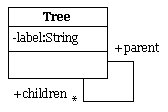
\includegraphics{images/metamodels/Tree.png}
	\caption{The Tree Metamodel}
	\label{fig:Tree1}
\end{figure}

As the Tree metamodel doesn't support a \emph{depth} property in the Tree metaclass, each Tree has to be associated with its calculated depth (line \ref{line:PutDepthInMap}) using the \emph{depths} map defined in line \ref{line:DeclareMap}. Another approach would be to extend the Tree metamodel to support the desired \emph{depth} property; however, applying this technique every time an additional property is needed for some model management operation would quickly pollute the metamodel with properties of secondary importance.

To simplify the code required in such cases, EOL provides the concept of \emph{extended properties}. In terms of concrete syntax, an extended property is a normal property, the name of which starts with the tilde character (\verb|~|). With regards to its execution semantics, the first time the value of an extended property of an object is assigned, the property is created and associated with the object. Then, the property can be accessed as a normal property. If an extended property is accessed before it is assigned, it returns \emph{null}. Listing \ref{lst:ExtendedProperties} demonstrates using a $~$\emph{depth} extended property to eliminate the need for using the \emph{depths} map in Listing \ref{lst:NoExtendedProperties}.

\begin{lstlisting}[float=tbp, caption=A simplified version of Listing \ref{lst:NoExtendedProperties} using extended properties, label=lst:ExtendedProperties, language=EOL]
for (n in Tree.allInstances.select(t|not t.parent.isDefined())) {
	n.setDepth(0);
}

for (n in Tree.allInstances) {
	(n.name + " " + n.~depth).println();
}

operation Tree setDepth(depth : Integer) {
	self.~depth = depth;
	for (c in self.children) {
		c.setDepth(depth + 1);
	}
}
\end{lstlisting}

%\section{Annotations}
%\label{sec:Design.EOL.Annotations}

\section{Context-Independent User Input}
\label{sec:Design.EOL.UserInput}

A common assumption in model management languages is that model management tasks are only executed in a batch-manner without human intervention. However, as demonstrated in the sequel, it is often useful for the user to provide feedback that can precisely drive the execution of a model management operation.

Model management operations can be executed in a number of runtime environments in each of which a different user-input method is more appropriate. For instance when executed in the context of an IDE (such as Eclipse) visual dialogs are preferable, while when executed in the context of a server or from within an ANT workflow, a command-line user input interface is deemed more suitable. To abstract away from the different runtime environments and enable the user to specify user interaction statements uniformly and regardless of the runtime context, EOL provides the \emph{IUserInput} interface that can be realized in different ways according to the execution environment and attached to the runtime context via the \emph{IEolContext.setUserInput(IUserInput userInput)} method. The \emph{IUserInput} specifies the methods presented in Table \ref{tab:IUserInputOperations}.

\begin{longtabu} {|p{6.5cm}|X|}
			
			\caption{Operations of IUserInput}
			\label{tab:IUserInputOperations}\\
			
			\hline
							
			\textbf{Signature} & \textbf{Description} \\\hline

			inform(message : String) & Displays the specified message to the user\\\hline
			
			confirm(message : String, [default : Boolean]) : Boolean & Prompts the user to confirm if the condition described by the message holds \\\hline
			
			prompt(message : String, [default : String]) : String & Prompts the user for a string in response to the message \\\hline
			
			promptInteger(message : String, [default : Integer]) : Integer & Prompts the user for an Integer \\\hline
			
			promptReal(message : String, [default : Real]) : Real & Prompts the user for a Real \\\hline
			
	 		choose(message : String, options : Sequence, [default : Any]) : Any & Prompts the user to select one of the options \\\hline
			
			chooseMany(message : String, options : Sequence, [default : Sequence]) : Sequence & Prompts the user to select one or more of the options \\\hline
			
\end{longtabu}

As displayed above, all the methods of the \emph{IUserInput} interface accept a \emph{default} parameter. The purpose of this parameter is dual. First, it enables the designer of the model management program to prompt the user with the most likely value as a default choice and secondly it enables a concrete implementation of the interface (\emph{UnattendedExecutionUserInput}) which returns the default values without prompting the user at all and thus, can be used for unattended execution of interactive Epsilon programs. Figures \ref{fig:EclipseUserInput} and \ref{fig:ConsoleUserInput} demonstrate the interfaces through which input is required by the user when the exemplar \emph{System.user.promptInteger('Please enter a number', 1);} statement is executed using  an Eclipse-based and a command-line-based \emph{IUserInput} implementation respectively.

\begin{figure}[b!]
	\centering
		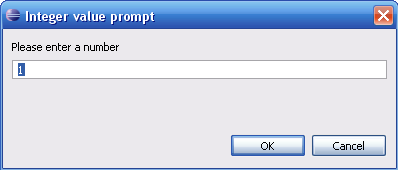
\includegraphics{images/EclipseUserInput.png}
	\caption{Example of an Eclipse-based IUserInput implementation}
	\label{fig:EclipseUserInput}
\end{figure}

\begin{figure}
	\centering
		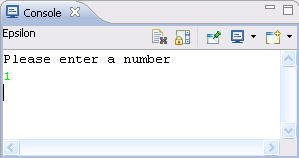
\includegraphics{images/ConsoleUserInput.png}
	\caption{Example of a command-line-based IUserInput implementation}
	\label{fig:ConsoleUserInput}
\end{figure}

User-input facilities have been found to be particularly useful in all model management tasks. Such facilities are essential for performing operations on live models such as model validation and model refactoring but can also be useful in model comparison where marginal matching decisions can be delegated to the user and model transformation where the user can interactively specify the elements that will be transformed into corresponding elements in the target model. Examples of interactive model management operations that make use of the input facilities provided by EOL are demonstrated in Sections \ref{sec:InteractiveModelTransformation} and \ref{sec:InteractiveModelComparison}



 %change to infrastructure

\section{Task-Specific Languages}
\label{sec:TaskSpecificLanguages}

Having discussed EOL in detail, in the following chapters, the following task-specific languages built atop EOL are presented:

\begin{itemize}
	\item Epsilon Validation Language (EVL)
	\item Epsilon Transformation Language (ETL)
	\item Epsilon Generation Language (EGL)
	\item Epsilon Wizard Language (EWL)
	\item Epsilon Comparison Language (ECL)
	\item Epsilon Merging Language (EML)
\end{itemize}

For each language, the abstract and concrete syntax are presented. To enhance readability, the concrete syntax of each language is presented in an abstract, pseudo-grammar form. Also provided is an informal but detailed discussion, accompanied by concise examples for each feature of interest, of its execution semantics and the runtime structures that are essential to implement those semantics.

Descriptions of the abstract and concrete syntaxes of the task-specific languages are particularly brief since they inherit most of their syntax and features from EOL. As discussed earlier, this contributes to establishing a platform of uniform languages where each provides a number of unique task-specific constructs but does not otherwise deviate from each other.

To reduce unnecessary repetition, the following sections do not repeat all the features inherited from EOL. However, the reader should bear in mind that by being supersets of EOL, all task-specific languages can exploit the features it provides. For example, by reusing EOL's user-input facilities (discussed in \ref{sec:Design.EOL.UserInput}), it is feasible to specify interactive model to model transformations in ETL. As well, \emph{Native} types can be used to access or update information stored in an external system/tool (e.g. in a database or a remote server) during model validation with EVL or model comparison with ECL.

Following the presentation, in Chapters \ref{sec:EVL} -- \ref{sec:EML}, of the task-specific languages implemented in Epsilon, Chapter \ref{sec:Design.ImplementingANewLanguage} provides a brief overview of the process needed to construct a new language that addresses a task that is not supported by one of the existing languages.

\chapter{The Epsilon Validation Language (EVL)}
\label{sec:EVL}

The aim of EVL is to contribute model validation capabilities to Epsilon. More specifically, EVL can be used to specify and evaluate constraints on models of arbitrary metamodels and modelling technologies. This section provides a discussion on the motivation for implementing EVL, its abstract and concrete syntax as well as its execution semantics. It also provides two examples using the language to verify inter-model and intra-model consistency.

\section{Motivation}
\label{sec:OCL.Limitations}

Although many approaches have been proposed to enable automated model validation, the Object Constraint Language (OCL) \cite{OCL} is the de facto standard for capturing constraints in modelling languages specified using object-oriented metamodelling technologies. While its powerful syntax enables users to specify meaningful and concise constraints, its purely declarative and side-effect free nature introduces a number of limitations in the context of a contemporary model management environment. In this section, the shortcomings of OCL that have motivated the design of EVL are discussed in detail.

In OCL, structural constraints are captured in the form of \textit{invariants}. Each invariant is defined in the context of a meta-class of the metamodel and specifies a name and a body. The body is an OCL expression that must evaluate to a \emph{Boolean} result, indicating whether an instance of the meta-class satisfies the invariant or not. Execution-wise, the body of each invariant is evaluated for each instance of the meta-class and the results are stored in a set of $<$Element, Invariant, Boolean$>$ triplets. Each triplet captures the \emph{Boolean} result of the evaluation of an \emph{Invariant} on a qualified \emph{Element}. An exemplar OCL invariant for UML 1.4, requiring that abstract operations only belong to abstract classes, is shown in Listing \ref{lst:AbstractOperations}.

\begin{lstlisting}[caption=OCL constraint on UML operations, label=lst:AbstractOperations, language=OCL]
context Operation
  inv AbstractOperationInAbstractClassOnly :
    self.isAbstract implies self.owner.isAbstract
\end{lstlisting}

While OCL enables users to capture particularly complex invariants, it also demonstrates a number of shortcomings, as follows.

\subsection{Limited user feedback}
\label{sec:Issue1}
OCL does not support specifying meaningful messages that can be reported to the user in case an invariant is not satisfied for certain elements. Therefore, feedback to the user is limited to the name of the invariant and the instance(s) for which it failed. Weak support for proper feedback messages implies that the end users must be familiar with OCL so that they can comprehend the meaning of the failed invariant and locate the exact reason for the failure. This is a significant shortcoming as in practice only a very small number of end users are familiar with OCL.

\subsection{No support for warnings/critiques}
\label{sec:Issue2}
Contemporary software development environments typically produce two types of feedback when checking artefacts for consistency and correctness: errors and warnings. Errors indicate critical deficiencies that contradict basic principles and invalidate the developed artefacts. By contrast, warnings (or critiques) indicate non-critical issues that should nevertheless be addressed by the user. To enable users to address warnings in a priority-based manner, they are typically categorized into three levels of importance: High, Medium and Low (although other classifications are also possible).

Nevertheless, in OCL there is no such distinction between errors and warnings and consequently all reported issues are considered to be errors. This adds an additional burden to identifying and prioritizing issues of major importance, particularly within an extensive set of unsatisfied invariants in complex models.

\subsection{No support for dependent constraints}
\label{sec:Issue3}
Each OCL invariant is a self-contained unit that does not depend on other invariants. There are cases where this design decision is particularly restrictive. For instance consider the invariants \emph{I1} and \emph{I2} displayed in Listing \ref{lst:RelatedConstraints}. Both I1 and I2 are applicable on UML classes with \emph{I1} requiring that: \textit{the name of a class must not be empty} and \emph{I2} requiring that: \textit{the name of a class must start with a capital letter}. In the case of those two invariants, if \emph{I1} is not satisfied for a particular UML class, evaluating \emph{I2} on that class would be meaningless. In fact it would be worse than meaningless since it would consume time to evaluate and would also produce an extraneous error message to the user. In practice, to avoid the extraneous message, \emph{I2} needs to replicate the body of \emph{I1} using an \textit{if} expression (lines 2 and 5).

\begin{lstlisting}[caption=Conceptually related OCL constraints, label=lst:RelatedConstraints, language=OCL]
context Class
	inv I1 : self.name.size() > 0
    	
  inv I2 : 
		if self.name.size > 0 then
			self.name.substring(0,1) =
			self.name.substring(0,1).toUpper()
		else
			true
		endif
\end{lstlisting}

\subsection{Limited flexibility in context definition}
\label{sec:Issue4}
As already discussed, in OCL invariants are defined in the context of meta-classes. While this achieves a reasonable partitioning of the model element space, there are cases where more fine-grained partitioning is required. For instance, consider the following scenario. Let $IA_{1..N}$, $IB_{1..M}$ be invariants applying to classes that are stereotyped as \verb|<<A>>| and \verb|<<B>>| respectively. Since OCL only supports partitioning the model element space using meta-classes, all $IA_{1..N}$, $IB_{1..M}$ must appear under the same context (i.e. \textit{Class}). Moreover, each invariant must explicitly define that it addresses the one or the other conceptual sub-partition. Therefore, each of $IA_{1..N}$ must limit its scope initially (using the $self.isA$ expression) and then express the real body. In our example the simplest way to achieve this would be by combining a scope-limiting expression with the real invariant body using the \textit{implies} clause as demonstrated in Listing \ref{lst:OCLDuplication}.

\begin{lstlisting}[float=t, caption=Demonstration of OCL constraints with duplication, label=lst:OCLDuplication, language=OCL2]
context Class
	inv I1 : self.isA implies <real-invariant-body>
	inv I2 : self.isA implies <real-invariant-body>
	...
	inv IN : self.isA implies <real-invariant-body>
	
	def isA :
		let isA : Boolean = 
		self.stereotype->exists(s|s.name = 'A')
\end{lstlisting}

Furthermore, if the \emph{real} body of the invariant needs to assume that self is stereotyped with \verb|<<A>>|, this technique is not applicable because OCL does not support lazy evaluation of Boolean clauses \cite{OCL} and therefore although the first part of the expression (\verb|self.isA|) may fail for some instances, the second part will still be evaluated thus producing runtime errors. In this case, an \textit{if} expression must be used, further complicating the specified invariants.

\subsection{No support for repairing inconsistencies} 
\label{sec:Issue5}
While OCL can be used for detecting inconsistencies, it provides no means for repairing them. The reason is that OCL has been designed as a side-effect free language and therefore lacks constructs for modifying models. Nevertheless, there are many cases where inconsistencies are trivial to resolve and users can benefit from semi-automatic repairing facilities. 

This need has been long recognized in the related field of code development tools (e.g. Eclipse, Microsoft Visual Studio, NetBeans). In such tools, errors are not only identified but also context-aware actions are proposed to the user for automatically repairing them. This feature significantly increases the usability of such tools and consequently enhances users' productivity.\\

\subsection{No support for inter-model constraints}
\label{sec:Issue6}
OCL expressions (and therefore OCL constraints) can only be evaluated in the context of a single model at a time. Consequently, OCL cannot be used to express constraints that span across different models. In the context of a large-scale model driven engineering process that involves many different models (that potentially conform to different modelling languages) this limitation is particularly severe.\\

\noindent Following this discussion on the shortcomings of OCL for capturing structural constraints in modelling languages, the following sections present the abstract and concrete syntax of EVL as well as their execution semantics, and explain how they address the aforementioned limitations.

\section{Abstract Syntax}

In EVL, validation specifications are organized in modules (\emph{EvlModule}). As illustrated in Figure \ref{fig:EvlAbstractSyntax}, \emph{EvlModule} extends \emph{EolLibraryModule} which means that it can contain user-defined operations and import other EOL library modules and EVL modules. Apart from operations, an EVL module also contains a set of invariants grouped by the context they apply to, and a number of \emph{pre} and \emph{post} blocks.

%\begin{landscape}
\begin{sidewaysfigure}
	\centering
	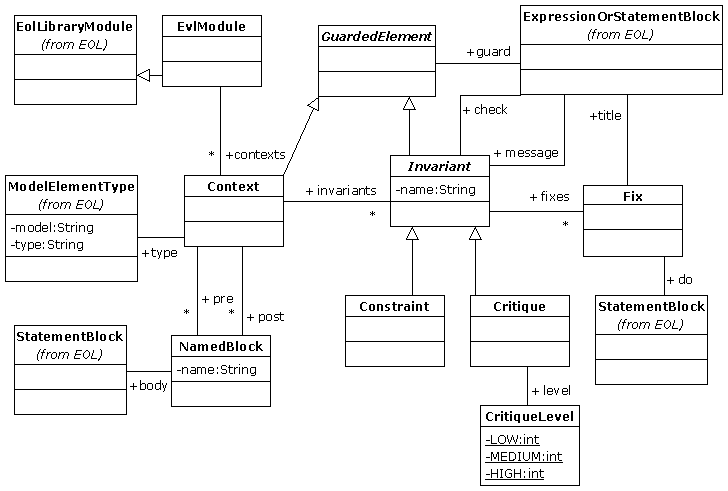
\includegraphics{images/EvlAbstractSyntax.png}
	\caption{Abstract Syntax of EVL}
	\label{fig:EvlAbstractSyntax}
\end{sidewaysfigure}
%\end{landscape}

\paragraph{Context} A context specifies the kind of instances on which the contained invariants will be evaluated. Each context can optionally define a guard which limits its applicability to a narrower subset of instances of its specified type. Thus, if the guard fails for a specific instance of the type, none of its contained invariants are evaluated.

\paragraph{Invariant} As with OCL, each EVL invariant defines a \emph{name} and a body (\emph{check}). However, it can optionally also define a \emph{guard} (defined in its abstract \emph{GuardedElement} supertype) which further limits its applicability to a subset of the instances of the type defined by the embracing \emph{context}. To achieve the requirement for detailed user feedback (Section \ref{sec:Issue1}), each invariant can optionally define a \emph{message} as an \emph{ExpressionOrStatementBlock} that should return a String providing a description of the reason(s) for which the constraint has failed on a particular element. To support semi-automatically fixing of elements on which invariants have failed (Section \ref{sec:Issue5}), an invariant can optionally define a number of \emph{fixes}. Finally, as displayed in Figure \ref{fig:EvlAbstractSyntax}, \emph{Invariant} is an abstract class that is used as a super-class for the specific types \emph{Constraint} and \emph{Critique}. This is to address the issue of separation of errors and warnings/critiques (Section \ref{sec:Issue2}).

\paragraph{Guard} Guards are used to limit the applicability of invariants (Section \ref{sec:Issue4}). This can be achieved at two levels. At the \emph{Context} level it limits the applicability of all invariants of the context and at the \emph{Invariant} level it limits the applicability of a specific invariant.

\paragraph{Fix}
A fix defines a title using an \emph{ExpressionOrStatementBlock} instead of a static String to allow users to specify context-aware titles (e.g. \emph{Rename class customer to Customer} instead of a generic \emph{Convert first letter to upper-case}). Moreover, the \emph{do} part is a statement block where the fixing functionality can be defined using EOL. The developer is responsible for ensuring that the actions contained in the \emph{fix} actually repair the identified inconsistency.

\paragraph{Constraint}
\emph{Constraints} in EVL are used to capture critical errors that invalidate the model. As discussed above, \emph{Constraint} is a sub-class of \emph{Invariant} and therefore inherits all its features.

\paragraph{Critique}
Unlike \emph{Constraints}, \emph{Critiques} are used to capture non-critical situations that do not invalidate the model, but should nevertheless be addressed by the user to enhance the quality of the model. This separation addresses the issue raised in Section \ref{sec:Issue2}.

\paragraph{Pre and Post}
An EVL module can define a number of named \emph{pre} and a \emph{post} blocks that contain EOL statements which are executed before and after evaluating the invariants respectively. These should not be confused with the pre-/post-condition annotations available for EOL user-defined operations (Section~\ref{sec:prep-cond-user}).

\section{Concrete Syntax}

Listings \ref{lst:ContextConcreteSyntax}, \ref{lst:InvariantConcreteSyntax} and \ref{lst:FixConcreteSyntax} demonstrate the concrete sytnax of the \emph{context}, \emph{invariant} and \emph{fix} abstract syntax constructs discussed above.

\begin{lstlisting}[caption=Concrete Syntax of an EVL context, label=lst:ContextConcreteSyntax, language=EVL, escapechar=!]
(@lazy)?
context !\textit{<name>}! !\textbf{\{}!

	(guard (!\textbf{:}\textit{expression}!)|(!\textbf{\{}\textit{statementBlock}\textbf{\}}!))?
	
	(!\textit{invariant}!)*
	
!\textbf{\}}!
\end{lstlisting}

\begin{lstlisting}[caption=Concrete Syntax of an EVL invariant, label=lst:InvariantConcreteSyntax, language=EVL, escapechar=!]
(@lazy)?
(constraint|critique) !\textit{<name>}! !\textbf{\{}!
	
	(guard (!\textbf{:}\textit{expression}!)|(!\textbf{\{}\textit{statementBlock}\textbf{\}}!))?
	
	(check (!\textbf{:}\textit{expression}!)|(!\textbf{\{}\textit{statementBlock}\textbf{\}}!))?
	
	(message (!\textbf{:}\textit{expression}!)|(!\textbf{\{}\textit{statementBlock}\textbf{\}}!))?
	
	(!\textit{fix}!)*
	
!\textbf{\}}
\end{lstlisting}

\begin{lstlisting}[float=t, caption=Concrete Syntax of an EVL fix, label=lst:FixConcreteSyntax, language=EVL, escapechar=!]
fix !\textbf{\{}!
	(guard (!\textbf{:}\textit{expression}!)|(!\textbf{\{}\textit{statementBlock}\textbf{\}}!))?
	
	(title (!\textbf{:}\textit{expression}!)|(!\textbf{\{}\textit{statementBlock}\textbf{\}}!))
	
	do !\textbf{\{}!
		!\textit{statementBlock}!
	!\textbf{\}}!
	
!\textbf{\}}!
\end{lstlisting}

\emph{Pre} and \emph{post} blocks have a simple syntax that, as presented in Listing \ref{lst:EvlPrePostConcreteSyntax}, consists of the identifier (\emph{pre} or \emph{post}), an optional name and the set of statements to be executed enclosed in curly braces.

\begin{lstlisting}[float=t, caption=Concrete Syntax of Pre and Post blocks, label=lst:EvlPrePostConcreteSyntax, language=EVL]
(pre|post) <name> {
	statement+
}
\end{lstlisting}

%\subsection{Concepts reused from EOL}

%As EVL has been built atop EOL, it reuses the following constructs from the base-language:

%\paragraph{ExpressionOrStatementBlock} There are cases where users needs to calculate a value (e.g. in the \emph{message} of an \emph{invariant}, in the \emph{guard} of a \emph{context} etc). When the value can be calculated declaratively, this is preferred. However, for cases in which calculating the value requires complex computations, users can use an EOL statement block and use a \emph{ReturnStatement} to return the calculated value to the caller.

%\paragraph{StatementBlock} A statement block is a sequence of EOL statements that can optionally include one or more \emph{ReturnStatements} to return a calculated value to its caller.

\section{Execution Semantics}
\label{sec:Design.EVL.ExecutionSemantics}

Having discussed the abstract and concrete syntaxes of EVL, this section provides an informal discussion of the execution semantics of the language. The execution of an EVL module is separated into four phases:

%The additional concepts EVL provides also affect its execution semantics. Currently, an EVL module can only be executed in batch-mode (all invariants against all instances). In the future we plan to investigate how the additional structures that EVL provides affect approaches to incremental consistency checking such as those presented in \cite{Cabot06,Egyed06}. In this section we outline the execution semantics of the language in batch-mode.

\paragraph{Phase 1} Before any invariant is evaluated, the \emph{pre} sections of the module are executed in the order in which they have been specified.

\paragraph {Phase 2} For each non-lazy \emph{context} with at least one non-lazy invariant, the instances of the meta-class it defines are collected. For each instance, the \emph{guard} of the \emph{context} is evaluated. If the \emph{guard} is satisfied, then for each non-lazy invariant contained in the context the invariant's \emph{guard} is also evaluated. If the \emph{guard} of the invariant is satisfied, the \emph{body} of the invariant is evaluated. In case the \emph{body} evaluates to \emph{false}, the \emph{message} part of the rule is evaluated and the produced message is added along with the instance, the invariant and the available \emph{fixes} to the \emph{ValidationTrace}.

The execution order of an EVL module follows a top-down depth-first scheme that respects the order in which the \emph{contexts} and \emph{invariants} appear in the module. However, the execution order can change in case one of the \emph{satisfies}, \emph{satisfiesOne}, \emph{satisfiesAll} built-in operations, discussed in detail in the sequel, are called.

\paragraph{Phase 3} In this phase, the validation trace is examined for unsatisfied constraints and the user is presented with the message each one has produced. The user can then select one or more of the available \emph{fixes} to be executed. Execution of \emph{fixes} is performed in a transactional manner using the respective facilities provided by the model connectivity framework, as discussed in Section \ref{sec:EMC.ModelTransactionSupport}. This is to prevent runtime errors raised during the execution of a \emph{fix} from compromising the validated model by leaving it in an inconsistent state.

\paragraph{Phase 4} When the user has performed all the necessary \emph{fixes} or chooses to end Phase 3 explicitly, the \emph{post} section of the module is executed. There, the user can perform tasks such as serializing the validation trace or producing a summary of the validation process results.

\subsection{Capturing Dependencies Between Invariants}

As discussed in Section \ref{sec:Issue3}, it is often the case that invariants conceptually depend on each other. To allow users capture such dependencies, EVL provides the \emph{satisfies(invariant : String) : Boolean}, \emph{satisfiesAll(invariants : Sequence(String)) : Boolean} and \emph{satisfiesOne(invariants : Sequence(String)) : Boolean} built-in operations. Using these operations, an invariant can specify in its \emph{guard} other invariants which need to be satisfied for it to be meaningful to evaluate.

When one of these operations is invoked, if the required \emph{invariants} (either lazy or non-lazy) have been evaluated for the instances on which the operation is invoked, the engine will return their cached results; otherwise it will evaluate them and return their results.

\section{Intra-Model Consistency Checking Example}
\label{sec:EvlIntraModelExample}
This section presents a case study comparing EVL and OCL in the context of a common scenario. The purpose of the case study is to present readers with the concrete syntax of the language and demonstrate the benefits delivered by the additional constructs it facilitates.

\subsection{Scenario: The Singleton Pattern}

The \emph{singleton} pattern is a widely used object oriented pattern. A \emph{singleton} is a class for which \emph{exactly one instance is allowed} \cite{Larman}. In UML, a singleton is typically represented as a class which is stereotyped with a \verb|<<singleton>>| stereotype and which also defines a static operation named \emph{getInstance()} that returns the unique instance. 

To ensure that all singletons have been modelled correctly in a UML model one needs to evaluate the following invariants on all classes that are stereotyped with the \verb|<<singleton>>| stereotype:

\begin{itemize}
	\item DefinesGetInstance : Each stereotyped class must define a getInstance() method
	\item GetInstanceIsStatic : The getInstance() method must be static
	\item GetInstanceReturnsSame : The return type of the getInstance() method must be the class itself 
\end{itemize}

Obviously, invariants \emph{GetInstanceIsStatic} and \emph{GetInstanceReturnsSame} depend on \emph{DefinesGetInstance} because if the singleton does not define a \emph{getInstance()} operation, checking for the operation's scope and return type is meaningless. Moreover, in case an invariant fails, there are corrective actions (fixes) that users may want to perform semi-automatically: e.g. for \emph{DefinesGetInstance}, such an action would be to add the missing \emph{getInstance()} operation, for \emph{GetInstanceIsStatic} to change it to static and for \emph{GetInstanceRetunrsSame} to set the return type to the class itself. In the following sections OCL and EVL are used to express the three constraints and then the two solutions are compared.

\subsection{Using OCL to Express the Invariants}

Listing \ref{lst:CaseStudyOcl} shows the aforementioned invariants implemented in OCL.

\begin{lstlisting}[basicstyle=\ttfamily\footnotesize, flexiblecolumns=true, numbers=none, nolol=true, caption=OCL Module for Validating Singletons, label=lst:CaseStudyOcl, numbers=left, language=OCL2, tabsize=2]
package Foundation::Core
    
		context Class 

		def isSingleton :
			let isSingleton : Boolean =
			self.stereotype->exists(s|s.name = 'singleton')
        
		def getInstanceOperation  : 
			let getInstanceOperation : Operation =
			self.feature->select(f|f.oclIsTypeOf(Operation) 
			and f.name = 'getInstance')->first().oclAsType(Operation)

		inv DefinesGetInstanceOperation : 
			if isSingleton 
				then getInstanceOperation.isDefined
				else true
			endif
    	
		inv GetInstanceOperationIsStatic :
			if isSingleton then
				if getInstanceOperation.isDefined 
					then getInstanceOperation.ownerScope = #classifier 
					else false
				endif
			else 
				true
			endif
    	
		inv GetOperationReturnsSame :
			if isSingleton then
				if getInstanceOperation.isDefined then
					if getInstanceOperation.returnParameter.isDefined
						then getInstanceOperation.returnParameter.type = self 
						else false
					endif
				else
					false
				endif
			else 
				true
			endif
    	
    context Operation
        
		def returnParameter :
			let returnParameter : Parameter =
			self.parameter->select(p|p.kind = #return)->first()

endpackage

\end{lstlisting}

By examining the OCL solution it can be observed that all invariants first check that the class is a singleton (lines 15, 21 and 31) by using the \emph{isSingleton} derived property defined in line 5. If the isSingleton returns \emph{false}, the invariants return \emph{true} since returning false would cause them to fail for all non-singleton classes. This reveals an additional shortcoming of OCL: if a constraint returns \emph{true} it may mean two different things: either that the instance satisfies the constraint or that the constraint is not applicable to the instance at all. In our view, this overloading reduces understandability.

By further studying the solution of Listing \ref{lst:CaseStudyOcl} it can be noticed that dependency between constraints is captured artificially using nested \emph{if} expressions. For instance, both \emph{GetInstanceIsStatic} and \emph{GetInstanceRetunrsSame} contain an \emph{if} expression in lines 22 and 32 respectively, requiring that they recalculate the value of the \emph{getInstanceOperation} defined in line 9, where they actually recalculate the result of the \emph{DefinesGetInstanceOperation} invariant. As discussed in Section \ref{sec:Issue3}, this happens because OCL lacks constructs for capturing dependencies in a structured manner.

\subsection{Using EVL to Express the Invariants}

Listing \ref{lst:CaseStudy} provides a solution for this problem expressed in EVL.

\begin{lstlisting}[basicstyle=\ttfamily\footnotesize, flexiblecolumns=true, numbers=none, nolol=true, caption=EVL Module for Validating Singletons, label=lst:CaseStudy, numbers=left, language=EVL, tabsize=2]
context Singleton typeOf Class {
	
	guard : self.stereotype->exists(s|s.name = 'singleton')
	
	constraint DefinesGetInstance {
		check : self.getGetInstanceOperation()->isDefined()
		message : 'Singleton ' + self.name + 
			' must define a getInstance() operation'
		fix {
			title : 'Add a getInstance() operation to ' + self.name
			do {
				-- Create the getInstance operation
				var op : new Operation;
				op.name := 'getInstance';
				op.owner := self;
				op.ownerScope := ScopeKind#sk_classifier;
				
				-- Create the return parameter
				var returnParameter : new Parameter;
				returnParameter.type := self;
				op.parameter := Sequence{returnParameter};
				returnParameter.kind := ParameterDirectionKind#pdk_return;
			}
		}
	}
	
	constraint GetInstanceIsStatic {
		guard : self.satisfies('DefinesGetInstance')
		check : self.getGetInstanceOperation().ownerScope = 
		        ScopeKind#sk_classifier
		message : ' The getInstance() operation of singleton ' 
		          + self.name + ' must be static'
	
		fix {
			title : 'Change to static'
			do {
				self.getGetInstanceOperation.ownerScope 
				  := ScopeKind#sk_classifier;
			}
		}
	}
	
	constraint GetInstanceReturnsSame {
	
		guard : self.satisfies('DefinesGetInstance')
		check {
			var returnParameter : Parameter;
			returnParameter := self.getReturnParameter();
			return (returnParameter->isDefined() 
			        and returnParameter.type = self);
		}
		message : ' The getInstance() operation of singleton ' 
		          + self.name + ' must return ' + self.name
			
		fix {
			title : 'Change return type to ' + self.name
			do {
				var returnParameter : Parameter;
				returnParameter := self.getReturnParameter();
				
				-- If the operation does not have a return parameter
				-- create one
				if (not returnParameter.isDefined()){
					returnParameter := Parameter.newInstance();
					returnParameter.kind := ParameterDirectionKind#pdk_return;
					returnParameter.behavioralFeature := 
						self.getInstanceOperation();
				}
				-- Set the correct return type
				returnParameter.type := self;
			}
		}
	}
}

operation Class getGetInstanceOperation() : Operation {
	return self.feature->
		select(o:Operation|o.name = 'getInstance').first();
}

operation Operation getReturnParameter() : Parameter {
	return self.parameter->
		select(p:Parameter|p.kind = 
			ParameterDirectionKind#pdk_return).first();
}
\end{lstlisting}

The \emph{Singleton} context defines that the invariants it contains will be evaluated on instances of the UML \emph{Class} type. Moreover, its guard defines that they will be evaluated only on classes that are stereotyped with the \emph{singleton} stereotype. Therefore, unlike the OCL solution of Listing \ref{lst:CaseStudyOcl}, invariants contained in this context do not need to check individually that the instances on which they are evaluated are singletons.

Constraint \emph{DefinesGetInstance} defines no guard which means that it will be evaluated for all the instances of the context. In its \emph{check} part, the constraint examines if the class defines an operation named \emph{getInstance()} by invoking the \emph{getGetInstanceOperation()} operation. If this fails, it proposes a fix that adds the missing operation to the class.

Constraint \emph{GetInstanceIsStatic} defines a guard which states that for the constraint to be evaluated on an instance, the instance must first satisfy the \emph{DefinesGetInstance} constraint. If it doesn't, it is not evaluated at all. In its \emph{check} part it examines that the \emph{getInstance()} operation is static. Note that here the constraint needs not check that the \emph{getInstance()} operation is defined again since this is assumed by the \emph{DefinesGetInstance} constraint on which it depends. If the constraint fails for an instance, the fix part can be invoked to change the scope of the \emph{getInstance()} operation to static.

Constraint \emph{GetInstanceReturnsSame} checks that the return type of the \emph{getInstance()} operation is the singleton itself. Similarly to the \emph{GetInstanceIsStatic} constraint, it defines that to be evaluated the \emph{DefinesGetInstance} constraint must be satisfied. If it fails for a particular instance, the fix part can be invoked. In the fix part, if the operation defines a return parameter of incorrect type, its type is changed and if it does not define a return parameter at all, the parameter is created and added to the parameters of the operation.

By observing the two solutions the OCL solution resembles the concept of defensive programming, where conditions are embedded in supplier code, while the EVL one is closer to the design by contract \cite{Meyer97} approach where conditions are explicitly checked in guards.

This case study has demonstrated that the additional constructs provided by EVL can reduce repetition significantly and thus enable specification of more concise constraints. Moreover, in case a constraint is not satisfied for a particular instance, the user is provided with a meaningful context-aware message and with automated facilities (fixes) for repairing the inconsistency.

\section{Inter-Model Consistency Checking Example}
\label{sec:EvlInterModelExample}

\begin{figure}[b]
	\centering
		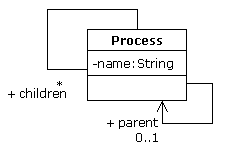
\includegraphics{images/Process.png}
	\caption{The ProcessLang Metamodel}
	\label{fig:Process}
\end{figure}

In the previous example, EVL was used to check the internal consistency of a single UML model. By contrast, this example demonstrates using EVL to detect and repair occurrences of incompleteness and contradiction between two different models. In this example the simplified \emph{ProcessLang} metamodel, which captures information about hierarchical processes, is used. To add performance information in a separate aspect \emph{ProcessPerformanceLang} metamodel is also defined. The metamodels are displayed in Figures \ref{fig:Process} and \ref{fig:ProcessPerformance} respectively.

\begin{figure}[h]
	\centering
		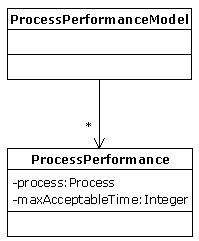
\includegraphics[width=0.2\textwidth]{images/ProcessPerformance.png}
	\caption{The ProcessPerformanceLang Metamodel}
	\label{fig:ProcessPerformance}
\end{figure}

There are two constraints that need to be defined and evaluated in this example: that each \emph{Process} in a process model (\emph{PM}) has a corresponding \emph{ProcessPerformance} in the process performance model (\emph{PPM}), and that the \emph{maxAcceptableTime} of a process does not exceed the sum of the \emph{maxAcceptableTimes} of its children. This is achieved with the \emph{PerformanceIsDefined} and the \emph{PerformanceIsValid} EVL constraints displayed in Listing \ref{lst:InterModelCaseStudy}.


\begin{lstlisting}[caption=Exemplar EVL module containing a cross-model constraint, label=lst:InterModelCaseStudy, language=EVL]
context PM!Process {	
	constraint PerformanceIsDefined { /*@\label{CaseStudy:PerformanceIsDefined}@*/
		
		check { /*@\label{CaseStudy:PerformanceIsDefined:Check}@*/
			var processPerformances = 
				PPM!ProcessPerformance.
				allInstances.select(pt|pt.process = self);
			
			return processPerformances.size() = 1;
		}
		
		message { /*@\label{CaseStudy:PerformanceIsDefined:Message}@*/
			var prefix : String;
			if (processPerformances.size() = 1) {
				prefix = "More than one performance info"; 
			}
			else {
				prefix = "No performance info";
			}
			return prefix + " found for process " 
				+ self.name;
		}
		
		fix { /*@\label{CaseStudy:PerformanceIsDefined:Fix}@*/
			title : "Set the performance of " + self.name
			
			do {
				for (p in processPerformances.clone()) {
					delete p;
				}
				var maxAcceptableTime : Integer;
				maxAcceptableTime = UserInput. /*@\label{CaseStudy:PerformanceIsDefined:Fix:Prompt}@*/
					promptInteger("maxAcceptableTime", 0); 
				var p : 
					new PPM!ProcessPerformance;
				p.maxAcceptableTime = maxAcceptableTime;
				p.process = self;
			}
		}
	}
	
	constraint PerformanceIsValid { /*@\label{CaseStudy:PerformanceIsValid}@*/
		
		guard : self.satisfies("PerformanceIsDefined") /*@\label{CaseStudy:PerformanceIsValid:Guard}@*/
			and self.children.forAll
				(c|c.satisfies("PerformanceIsDefined"))
		
		check { /*@\label{CaseStudy:PerformanceIsValid:Check}@*/
			var sum : Integer;
			sum = self.children. /*@\label{CaseStudy:PerformanceIsValid:Sum}@*/
				collect(c|c.getMaxAcceptableTime()) 
				.sum().asInteger(); 
			return self.getMaxAcceptableTime() >= sum;
		}
		
		message : "Process " + self.name + /*@\label{CaseStudy:PerformanceIsValid:Message}@*/
			" has a smaller maxAcceptableTime " 
			+ "than the sum of its children"
		
		fix { /*@\label{CaseStudy:PerformanceIsValid:Fix}@*/
			title : "Increase maxAcceptableTime to " + sum
			do {
				self.setMaxAcceptableTime(sum);
			}
		}
		
	}
	
}

operation PM!Process getMaxAcceptableTime() /*@\label{CaseStudy:getMaxAcceptableTime}@*/
	: Integer { 
	return PPM!ProcessPerformance.
		allInstances.selectOne(pt|pt.process=self)
			.maxAcceptableTime;
}

operation PM!Process setMaxAcceptableTime /*@\label{CaseStudy:setMaxAcceptableTime}@*/
	(time : Integer) { 
	PPM!ProcessPerformance.allInstances.
		selectOne(pt|pt.process=self).maxAcceptableTime =
		time;
}
\end{lstlisting}

In line \ref{CaseStudy:PerformanceIsDefined:Check}, the check part of the \emph{PerformanceIsDefined} constraint calculates the instances of \emph{ProcessPerformance} in the \emph{ProcessPerformanceModel} that have their \emph{process} reference set to the currently examined \emph{Process} (accessible via the \emph{self} built-in variable) and stores it in the \emph{processPerformances} variable. If exactly one \emph{ProcessPerformance} is defined for the \emph{Process}, the constraint is satisfied. Otherwise, the \emph{message} part of the constraint, in line \ref{CaseStudy:PerformanceIsDefined:Message}, is evaluated and an appropriate error message is displayed to the user. 

Note that the \emph{processPerformances} variable defined in the \emph{check} part is also used from within the \emph{message} part of the constraint. As discussed in \cite{EVL}, EVL provides this feature to reduce the need for duplicate calculations as our experience has shown that the message for a failed constraint often needs to utilize side-information collected in the \emph{check} part.

To repair the inconsistency, the user can invoke the \emph{fix} defined in line \ref{CaseStudy:PerformanceIsDefined:Fix} that will delete any existing \emph{ProcessPerformance} instances and create a new one with a user-defined \emph{maxAcceptableTime} obtained using the \emph{UserInput.promptInteger()} statement of line \ref{CaseStudy:PerformanceIsDefined:Fix:Prompt}.

Unlike the \emph{PerformanceIsDefined} constraint, the \emph{PerformanceIsValid} constraint, line \ref{CaseStudy:PerformanceIsValid}, defines a \emph{guard} part (line \ref{CaseStudy:PerformanceIsValid:Guard}). As discussed in \cite{EVL}, the guard part of a constraint is used to further limit the applicability of the constraint beyond the simple type check performed in the containing \emph{context}. In this rule, the validity of the \emph{maxAcceptableTime} of a \emph{Process} needs to be checked only if one has been defined in the \emph{ProcessPerformanceModel}. Therefore, the guard part of the constraint specifies that this constraint is only applicable to \emph{Processes} where, both they and they children, satisfy the \emph{PerformanceIsDefined} constraint.

The check part of the constraint retrieves the \emph{maxAcceptableTime} of the process and that of its children and compares them. As the \emph{Process} itself does not define performance information, retrieval of the value of the \emph{maxAcceptableTime} of the respective \emph{ProcessPerformance} object is implemented using the user-defined \emph{getMaxAcceptableTime()} operation that is defined in line \ref{CaseStudy:getMaxAcceptableTime}. In case the constraint is not satisfied, the user can invoke the \emph{fix} defined in line \ref{CaseStudy:PerformanceIsValid:Fix} to repair the inconsistency by setting the \emph{maxAcceptableTime} of the process to the \emph{sum} calculated in line \ref{CaseStudy:PerformanceIsValid:Sum}. As discussed earlier, the fix parts of EVL invariants do not in any way guarantee that they do fix the problem they target or that in their effort to fix one problem they do not create another problem; this is left to the user. For instance, in this particular example, changing the \emph{maxAcceptableTime} of a process through a \emph{fix} block may render its parent process invalid.


To demonstrate the evaluation of these constraints two exemplar models that conform to the \emph{ProcessLang} and \emph{ProcessPerformanceLang} metamodels are used. A visual representation of the models is displayed in Figure \ref{fig:ModeLink}.

\begin{figure}[h]
    \centering
    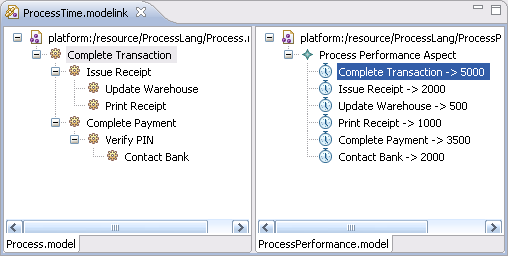
\includegraphics{images/ModeLink.png}
    \caption{Exemplar Process and ProcessPerformance models}
    \label{fig:ModeLink}
\end{figure}


Evaluating the constraints in the context of those two models reveals two problems which are reported to the user via the view displayed in Figure \ref{fig:Validation}. Indeed by examining the two models of Figure \ref{fig:ModeLink}, it becomes apparent that there is no \emph{ProcessPerformance} linked to the \emph{Verify PIN} process and also that the \emph{maxAcceptableTime} of \emph{Complete Transaction} (5000) is less than the sum of the \emph{maxAcceptableTimes} of its children (2000 + 3500).

\begin{figure}[h]
    \centering
    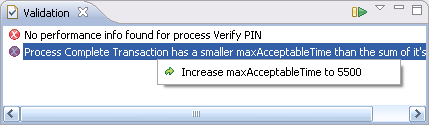
\includegraphics{images/Validation.png}
    \caption{Screenshot of the validation view reporting the identified inconsistencies}
    \label{fig:Validation}
\end{figure}

\section{Summary}

This section has provided a detailed discussion on the EVL model-validation language which conceptually (as opposed to technically) extends OCL. EVL provides a number of features such as support for detailed user feedback, constraint dependency management, semi-automatic transactional inconsistency resolution and (as it is based on EOL) access to multiple models of diverse metamodels and technologies.

%%% Local Variables:
%%% mode: latex
%%% TeX-master: "EpsilonBook"
%%% End:


\chapter{The Epsilon Transformation Language (ETL)}
\label{sec:ETL}

The aim of ETL \cite{ETL} is to contribute model-to-model transformation capabilities to Epsilon. More specifically, ETL can be used to transform an arbitrary number of input models into an arbitrary number of output models of different modelling languages and technologies at a high level of abstraction. 

\section{Style}

Three styles are generally recognized in model transformation languages: declarative, imperative and hybrid, each one demonstrating particular advantages and shortcomings. Declarative transformation languages are generally limited to scenarios where the source and target metamodels are similar to each other in terms of structure and thus, the transformation is a matter of a simple mapping. However they fail to address cases where significant processing and complex mappings are involved. On the other hand, purely imperative transformation languages are capable of addressing a wider range of transformation scenarios. Nevertheless, they operate at a low level of abstraction which means that users need to manually address issues such as tracing and resolving target elements from their source counterparts and orchestrating the transformation execution. To address those shortcomings, hybrid languages (such as ATL \cite{ATL} and QVT \cite{QVT}) provide both a declarative rule-based execution scheme as well as imperative features for handling complex transformation scenarios. 

Under this rationale, ETL has been designed as a hybrid language that implements a task-specific rule definition and execution scheme but also inherits the imperative features of EOL to handle complex transformations where this is deemed necessary.

\section{Source and Target Models}

The majority of model-to-model transformation languages assume that only two models participate in each transformation: the source model and the target model. Nevertheless, it is often essential to be able to access/update additional models during a transformation (such as trace or configuration models). Building on the facilities provided by EMC and EOL, ETL enables specification of transformations that can transform an arbitrary number of source models into an arbitrary number of target models.

Another common assumption is that the contents of the target models are insignificant and thus a transformation can safely overwrite its contents. As discussed in the sequel, ETL - like all Epsilon languages - enables the user to specify, for each involved model, whether its contents need to be preserved or not.

\section{Abstract Syntax}

As illustrated in Figure \ref{fig:EtlAbstractSyntax}, ETL transformations are organized in modules (\emph{EtlModule}). A module can contain a number of transformation rules (\emph{TransformationRule}). Each rule has a unique name (in the context of the module) and also specifies one \emph{source} and many \emph{target} parameters. A transformation rule can also \emph{extend} a number of other transformation rules and be declared as \emph{abstract}, \emph{primary} and/or \emph{lazy}\footnote{The concept of lazy rules was first introduced in ATL}. To limit its applicability to a subset of elements that conform to the type of the \emph{source} parameter, a rule can optionally define a guard which is either an EOL expression or a block of EOL statements. Finally, each rule defines a block of EOL statements (\emph{body}) where the logic for populating the property values of the target model elements is specified.

Besides transformation rules, an ETL module can also optionally contain a number of \emph{pre} and \emph{post} named blocks of EOL statements which, as discussed later, are executed before and after the transformation rules respectively. These should not be confused with the pre-/post-condition annotations available for EOL user-defined operations (Section~\ref{sec:prep-cond-user}).

\begin{landscape}
\begin{figure}
	\centering
		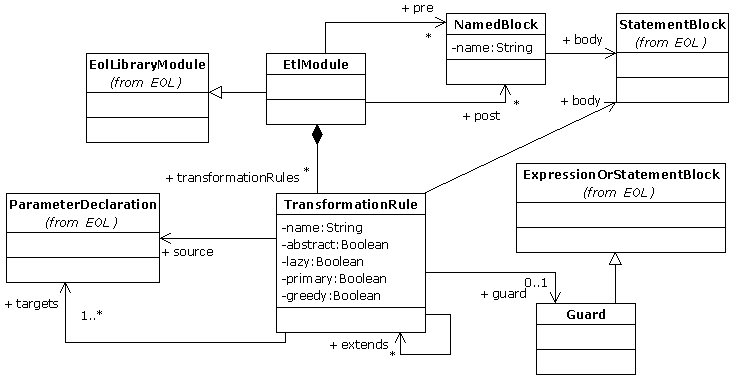
\includegraphics{images/EtlAbstractSyntax.png}
	\caption{ETL Abstract Syntax}
	\label{fig:EtlAbstractSyntax}
\end{figure}
\end{landscape}

\section{Concrete Syntax}

The concrete syntax of a transformation rule is displayed in Listing \ref{lst:TransformationRuleConcreteSyntax}. The optional \emph{abstract}, \emph{lazy} and \emph{primary} attributes of the rule are specified using respective annotations. The name of the rule follows the \emph{rule} keyword and the \emph{source} and \emph{target} parameters are defined after the \emph{transform} and \emph{to} keywords. Also, the rule can define an optional comma-separated list of rules it extends after the \emph{extends} keyword. Inside the curly braces (\{\}), the rule can optionally specify its \emph{guard} either as an EOL expression following a colon (:) (for simple guards) or as a block of statements in curly braces (for more complex guards). Finally, the \emph{body} of the rule is specified as a sequence of EOL statements.

\begin{lstlisting}[caption=Concrete Syntax of a TransformationRule, label=lst:TransformationRuleConcreteSyntax, language=ETL]
(@abstract)?
(@lazy)?
(@primary)?
rule <name> 
	transform <sourceParameterName>:<sourceParameterType>
	to (<rightParameterName>:<rightParameterType>
	(, <rightParameterName>:<rightParameterType>)*
	(extends (<ruleName>,)*<ruleName>)? {
	
	(guard (:expression)|({statement+}))?
	
	statement+
}
\end{lstlisting}

\emph{Pre} and \emph{post} blocks have a simple syntax that, as presented in Listing \ref{lst:EtlPrePostConcreteSyntax}, consists of the identifier (\emph{pre} or \emph{post}), an optional name and the set of statements to be executed enclosed in curly braces.

\begin{lstlisting}[caption=Concrete Syntax of Pre and Post blocks, label=lst:EtlPrePostConcreteSyntax, language=ETL]
(pre|post) <name> {
	statement+
}
\end{lstlisting}

\section{Execution Semantics}
\label{sec:ETL.ExecutionSemantics}

\subsection{Rule and Block Overriding}
Similarly to ECL, an ETL module can import a number of other ETL modules. In this case, the importing ETL module inherits all the rules and pre/post blocks specified in the modules it imports (recursively). If the module specifies a rule or a pre/post block with the same name, the local rule/block overrides the imported one respectively.

\subsection{Rule Execution Scheduling}

When an ETL module is executed, the \emph{pre} blocks of the module are executed first in the order in which they have been specified. 

Following that, each \emph{non-abstract} and \emph{non-lazy} rule is executed for all the elements on which it is applicable. To be applicable on a particular element, the element must have a kind-of relationship with the type defined in the rule's \emph{sourceParameter} and must also satisfy the \emph{guard} of the rule (and all the rules it extends). When a rule is executed on an applicable element, the target elements are initially created by instantiating the \emph{targetParameters} of the rules, and then their contents are populated using the EOL statements of the \emph{body} of the rule.

Finally, when all rules have been executed, the \emph{post} blocks of the module are executed in the order in which they have been declared.

\subsection{Source Elements Resolution}

Resolving target elements that have (or can be) transformed from source elements by other rules is a frequent task in the body of a transformation rule. To automate this task and reduce coupling between rules, ETL contributes the \emph{equivalents()} and \emph{equivalent()} built-in operations that automatically resolve source elements to their transformed counterparts in the target models. 

When the \emph{equivalents()} operation is applied on a single source element (as opposed to a collection of them), it inspects the established transformation trace (displayed in Figure \ref{fig:EtlRuntime}) and invokes the applicable rules (if necessary) to calculate the counterparts of the element in the target model. When applied to a collection it returns a \emph{Bag} containing \emph{Bags} that in turn contain the counterparts of the source elements contained in the collection. The \emph{equivalents()} operation can be also invoked with an arbitrary number of rule names as parameters to invoke and return only the equivalents created by specific rules. Unlike the main execution scheduling scheme discussed above, the \emph{equivalents()} operation invokes both \emph{lazy} and \emph{non-lazy} rules. It is worth noting that \emph{lazy} rules are computationally expensive and should be used with caution as they can significantly degrade the performance of the overall transformation.

With regard to the ordering of the results of the \emph{equivalents()} operations, the returned elements appear in the respective order of the rules that have created them. An exception to this occurs when one of the rules is declared as \emph{primary}, in which case its results precede the results of all other rules.

\begin{landscape}
\begin{figure}
	\centering
		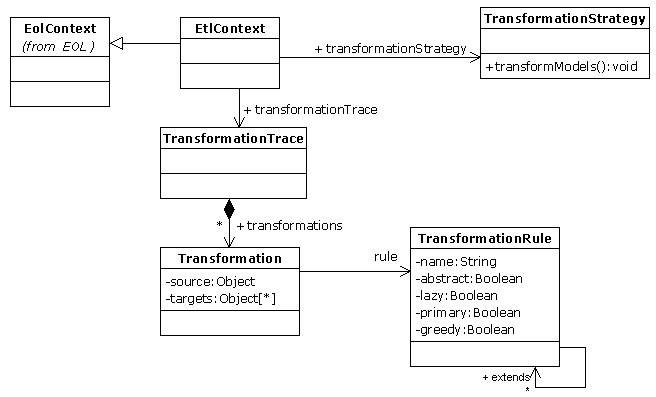
\includegraphics{images/EtlRuntime.png}
	\caption{ETL Runtime}
	\label{fig:EtlRuntime}
\end{figure}
\end{landscape}


ETL also provides the convenience \emph{equivalent()} operation which, when applied to a single element, returns only the first element of the respective result that would have been returned by the \emph{equivalents()} operation discussed above. Also, when applied to a collection the \emph{equivalent()} operation returns a flattened collection (as opposed to the result of \emph{equivalents()} which is a \emph{Bag} of \emph{Bags} in this case). As with the \emph{equivalents()} operation, the \emph{equivalent()} operation can also be invoked with or without parameters.

The semantics of the \emph{equivalent()} operation are further illustrated through a simple example. In this example, we need to transform a model that conforms to the Tree metamodel displayed in Figure \ref{fig:Tree} into a model that conforms to the Graph metamodel of Figure \ref{fig:Graph}. More specifically, we need to transform each \emph{Tree} element to a \emph{Node}, and an \emph{Edge} that connects it with the \emph{Node} that is equivalent to the tree's \emph{parent}. This is achieved using the rule of Listing \ref{lst:SimpleETLTransformationRule}. 

\begin{lstlisting}[float=h, caption=Exemplar ETL Rule demonstrating the \emph{equivalent()} operation, label=lst:SimpleETLTransformationRule, language=ETL, escapechar=\#]
rule Tree2Node#\label{lst:etl-simple-def-start}#
	transform t : Tree!Tree
	to n : Graph!Node {#\label{lst:etl-simple-def-end}#
	
	n.label = t.label;#\label{lst:etl-simple-label}#
	
	if (t.parent.isDefined()) {#\label{lst:etl-simple-sourceisdef}#
		var edge = new Graph!Edge;#\label{lst:etl-simple-newedge}#
		edge.source = n;#\label{lst:etl-simple-source}#
		edge.target = t.parent.equivalent();#\label{lst:etl-simple-equiv}#
	}
}
\end{lstlisting}


In lines \ref{lst:etl-simple-def-start}--\ref{lst:etl-simple-def-end}, the \emph{Tree2Node} rule specifies that it can transform elements of the \emph{Tree} type in the \emph{Tree} model into elements of the \emph{Node} type in the \emph{Graph} model. In line~\ref{lst:etl-simple-label} it specifies that the name of the created Node should be the same as the name of the source Tree. If the parent of the source \emph{Tree} is defined (line~\ref{lst:etl-simple-sourceisdef}), the rule creates a new \emph{Edge} (line~\ref{lst:etl-simple-newedge}) and sets its \emph{source} property to the created \emph{Node} (line~\ref{lst:etl-simple-source}) and its \emph{target} property to the \emph{equivalent} \emph{Node} of the source \emph{Tree}'s \emph{parent} (line~\ref{lst:etl-simple-equiv}).

\begin{figure}
	\centering
		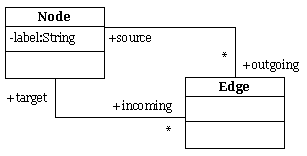
\includegraphics{images/Graph.png}
	\caption{A Simple Graph Metamodel}
	\label{fig:Graph}
\end{figure}


\subsection{Overriding the semantics of the EOL SpecialAssignmentOperator}
\label{sec:Design.ETL.SpecialAssignmentOperator}

As discussed above, resolving the equivalent(s) or source model elements in the target model is a recurring task in model transformation. Furthermore, in most cases resolving the equivalent of a model element is immediately followed by assigning/adding the obtained target model elements to the value(s) of a property of another target model element. For example, in line 10 of Listing \ref{lst:SimpleETLTransformationRule} the \emph{equivalent} obtained is immediately assigned to the \emph{target} property of the generated \emph{Edge}. To make transformation specifications more readable, ETL overrides the semantics of the \emph{SpecialAssignmentStatement} (\emph{::=} in terms of concrete syntax), described in Section \ref{sec:Design.EOL.SpecialAssignmentStatement} to set its left-hand side, not to the element its right-hand side evaluates to, but to its \emph{equivalent} as calculated using the \emph{equivalent()} operation discussed above. Using this feature, line 10 of the \emph{Tree2Node} rule can be rewritten as shown in Listing \ref{lst:SpecialAssignmentETLTransformationRule}

\begin{lstlisting}[caption=Rewritten Line 10 of the \emph{Tree2Node} Rule Demonstrated in Listing \ref{lst:SimpleETLTransformationRule}, label=lst:SpecialAssignmentETLTransformationRule, language=ETL]
edge.target ::= t.parent;
\end{lstlisting}


\section{Interactive Transformations}
\label{sec:InteractiveModelTransformation}

Using the user interaction facilities of EOL discussed in Section \ref{sec:Design.EOL.UserInput}, an ETL transformation can become interactive by prompting the user for input during its execution. For example in Listing \ref{lst:InteractiveETLTransformationRule}, we modify the \emph{Tree2Node} rule originally presented in Listing \ref{lst:SimpleETLTransformationRule} by adding a \emph{guard} part that uses the user-input facilities of EOL (more specifically the \emph{UserInput.confirm(String,Boolean)} operation) to enable the user select manually at runtime which of the Tree elements need to be transformed to respective Node elements in the target model and which not. 

\begin{lstlisting}[caption=Exemplar Interactive ETL Transformation, label=lst:InteractiveETLTransformationRule, language=ETL]
rule Tree2Node
	transform t : Tree!Tree
	to n : Graph!Node {
	
	guard : UserInput.confirm
		("Transform tree " + t.label + "?", true)
	
	n.label = t.label;
	var target : Graph!Node ::= t.parent;
	if (target.isDefined()) {
		var edge = new Graph!Edge;
		edge.source = n;
		edge.target = target;
	}
}
\end{lstlisting}

\section{Summary}

This section has provided a detailed discussion on the Epsilon Transformation Language (ETL). ETL is capable of transforming an arbitrary number of source models into an arbitrary number of target models. ETL adopts a hybrid style and features declarative rule specification using advanced concepts such as \emph{guards}, \emph{abstract}, \emph{lazy} and \emph{primary} rules, and automatic resolution of target elements from their source counterparts. Also, as ETL is based on EOL reuses its imperative features to enable users to specify particularly complex, and even interactive, transformations.

\chapter{The Epsilon Wizard Language (EWL)}
\label{sec:EWL}

There are two types of model-to-model transformations: mapping and update transformations \cite{Czarnecki2003}. Mapping transformations typically transform a source model into a set of target models expressed in (potentially) different modelling languages by creating zero or more model elements in the target models for each model element of the source model. By contrast, update transformations perform in-place modifications in the source model itself. They can be further classified into two subcategories: transformations in the small and in the large. Update transformations in the large apply to sets of model elements calculated using well-defined rules in a batch manner. An example of this category of transformations is a transformation that automatically adds accessor and mutator operations for all attributes in a UML model. On the other hand, update transformations in the small are applied in a user-driven manner on model elements that have been explicitly selected by the user. An example of this kind of transformations is a transformation that renames a \emph{user-specified} UML class and all its incoming associations consistently.

In Epsilon, mapping transformations can be specified using ETL as discussed in Section \ref{sec:ETL}, and update transformations in the large can be implemented either using the model modification features of EOL or using an ETL transformation in which the source and target models are the same model. By contrast, update transformations in the small cannot be effectively addressed by any of the languages presented so far.

The following section discusses the importance of update transformations in the small and motivates the definition of a task-specific language (Epsilon Wizard Language (EWL)) that provides tailored and effective support for defining and executing update transformations on models of diverse metamodels.

\section{Motivation}
\label{sec:EwlMotivation}

Constructing and refactoring models is undoubtedly a mentally intensive process. However, during modelling, recurring patterns of model update activities typically appear. As an example, when renaming a class in a UML class diagram, the user also needs to manually update the names of association ends that link to the renamed class. Thus, when renaming a class from \emph{Chapter} to \emph{Section}, all associations ends that point to the class and are named \emph{chapter} or \emph{chapters} should be also renamed to \emph{section} and \emph{sections} respectively. As another example, when a modeller needs to refactor a UML class into a singleton \cite{Larman}, they need to go through a number of well-defined, but trivial, steps such as attaching a stereotype ($<<singleton>>$), defining a static \emph{instance} attribute and adding a static \emph{getInstance()} method that returns the unique instance of the singleton.

It is generally accepted that performing repetitive tasks manually is both counter-productive and error-prone \cite{CG.InAction}. On the other hand, failing to complete such tasks correctly and precisely compromises the consistency, and thus the quality, of the models. In Model Driven Engineering, this is particularly important since models are increasingly used to automatically produce (parts of) working systems. 

\subsection{Automating the Construction and Refactoring Process}

Contemporary modelling tools provide built-in transformations (\textit{wizards}) for automating common repetitive tasks. However, according to the architecture of the designed system and the specific problem domain, additional repetitive tasks typically appear, which cannot be addressed by the pre-conceived built-in wizards of a modelling tool. To address the automation problem in its general case, users must be able to easily define update transformations (wizards) that are tailored to their specific needs.

To an extent, this can be achieved via the extensible architecture that state-of-the-art modelling tools often provide and which enables users to add functionality to the tool via scripts or application code using the implementation language of the tool. Nevertheless, as discussed in \cite{EOL}, the majority of modelling tools provide an API through which they expose an edited model, which requires significant effort to learn and use. Also, since each API is proprietary, such scripts and extensions are not portable to other tools. Finally, API scripting languages and third-generation languages such as Java and C++ are not particularly suitable for model navigation and modification \cite{EOL}.

Furthermore, existing languages for mapping transformations, such as QVT, ATL and ETL, cannot be used as-is for this purpose, because these languages have been designed to operate in a batch manner without human involvement in the process. By contrast, as discussed above, the task of constructing and refactoring models is inherently user-driven.

\section{Update Transformations in the Small}
\label{sec:ModelTransformationInTheSmall}

Update transformations are actions that automatically create, update or delete model elements based on a selection of existing elements in the model and information obtained otherwise (e.g. through user input), in a user-driven fashion. In this section such actions are referred to as \textit{wizards} instead of \textit{rules} to reduce confusion between them and rules of mapping transformation languages. In the following sections the desirable characteristics of wizards are elaborated informally. 

\subsection{Structure of Wizards}

In its simplest form, a wizard only needs to define the actions it will perform when it is applied to a selection of model elements. The structure of such a wizard that transforms a UML class into a \textit{singleton} is shown using pseudo-code in Listing \ref{lst:Basic}.\\

\begin{lstlisting}[caption=The simplest form of a wizard for refactoring a class into a singleton, label=lst:Basic, language=EWL]
do :
	attach the singleton stereotype
	create the instance attribute
	create the getInstance method
\end{lstlisting}

Since not all wizards apply to all types of elements in the model, each wizard needs to specify the types of elements to which it applies. For example, the wizard of Listing \ref{lst:Basic}, which automatically transforms a class into a singleton, applies only when the selected model element is a class. The simplest approach to ensuring that the wizard will only be applied on classes is to enclose its body in an \emph{if} condition as shown in Listing \ref{lst:WithoutGuard}.

\begin{lstlisting}[caption=The wizard of Listing \ref{lst:Basic} enhanced with an $if$ condition, label=lst:WithoutGuard, language=EWL]
do : 
	if (selected element is a class) {
		attach the singleton stereotype
		create the instance attribute
		create the getInstance method
	}
\end{lstlisting}

A more modular approach is to separate this condition from the body of the wizard. This is shown in Listing \ref{lst:WithGuard} where the condition of the wizard is specified as a separate \emph{guard} stating that the wizard applies only to elements of type Class. The latter is preferable since it enables filtering out wizards that are not applicable to the current selection of elements by evaluating only their \emph{guard} parts and rejecting those that return \emph{false}. Thus, at any time, the user can be provided with only the wizards that are applicable to the current selection of elements. Filtering out irrelevant wizards reduces confusion and enhances usability, particularly as the list of specified wizards grows.

\begin{lstlisting}[caption=The wizard of Listing \ref{lst:WithoutGuard} with an explicit $guard$ instead of the $if$ condition, label=lst:WithGuard, language=EWL]
guard : selected element is a class
do : 
	attach the singleton stereotype
	create the instance attribute
	create the getInstance method
\end{lstlisting}

To enhance usability, a wizard also needs to define a short human-readable description of its functionality. To achieve this, another field named \emph{title} has been added. There are two options for defining the title of a wizard: the first is to use a static string and the second to use a dynamic expression. The latter is preferable since it enables definition of context-aware titles.

\begin{lstlisting}[caption=The wizard of Listing \ref{lst:WithGuard} enhanced with a $title$ part, label=lst:FinalForm, language=EWL]
guard : selected element is a class
title : Convert class <class-name> into a singleton
do : 
	attach the singleton stereotype
	create the instance attribute
	create the getInstance method
\end{lstlisting}

\subsection{Capabilities of Wizards}

The \emph{guard} and \emph{title} parts of a wizard need to be expressed using a language that provides model querying and navigation facilities. Moreover, the \emph{do} part also requires model modification capabilities to implement the transformation. To achieve complex transformations, it is essential that the user can provide additional information. For instance, to implement a wizard that addresses the class renaming scenario discussed in Section \ref{sec:EwlMotivation}, the information provided by the selected class does not suffice; the user must also provide the new name of the class. Therefore, EWL must also provide mechanisms for capturing user input.

\section{Abstract Syntax}

Since EWL is built atop Epsilon, its abstract and concrete syntax need only to define the concepts that are relevant to the task it addresses; they can reuse lower-level constructs from EOL. A graphical overview of the abstract syntax of the language is provided in Figure \ref{fig:EwlAbstractSyntax}. 

The basic concept of the EWL abstract syntax is a \emph{Wizard}. A wizard defines a \emph{name}, a \emph{guard} part, a \emph{title} part and a $do$ part. Wizards are organized in \emph{Modules}. The \emph{name} of a wizard acts as an identifier and must be unique in the context of a module. The \emph{guard} and \emph{title} parts of a wizard are of type \emph{ExpressionOrStatementBlock}, inherited from EOL. An \emph{ExpressionOrStatementBlock} is either a single EOL expression or a block of EOL statements that include one or more \emph{return} statements. This construct allows users to express simple declarative calculations as single expressions and complex calculations as blocks of imperative statements. The usefulness of this construct is further discussed in the examples presented in Section \ref{sec:EwlExamples}. Finally, the \emph{do} part of the wizard is a block of EOL statements that specify the effects of the wizard when applied to a compatible selection of model elements. 

\begin{figure}
	\centering
		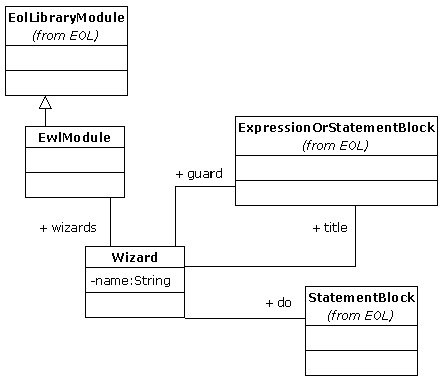
\includegraphics{images/EwlAbstractSyntax.png}
	\caption{EWL Abstract Syntax}
	\label{fig:EwlAbstractSyntax}
\end{figure}

\clearpage

\section{Concrete Syntax}

Listing \ref{lst:EwlConcreteSyntax} presents the concrete syntax of EWL wizards.

\begin{lstlisting}[caption=Concrete syntax of EWL wizards, label=lst:EwlConcreteSyntax, language=EWL]
wizard <name> {
	(guard (:expression)|({statementBlock}))?
	(title (:expression)|({statementBlock}))?
	do {
		statementBlock
	}
}
\end{lstlisting}

\section{Execution Semantics}
The process of executing EWL wizards is inherently user-driven and as such it depends on the environment in which they are used. In general, each time the selection of model elements changes (i.e. the user selects or deselects a model element in the modelling tool), the guards of all wizards are evaluated. If the guard of a wizard is satisfied, the \emph{title} part is also evaluated and the wizard is added to a list of \textit{applicable} wizards. Then, the user can select a wizard and execute its \emph{do} part to perform the intended transformation.

In EWL, variables defined and initialized in the \emph{guard} part of the wizard can be accessed both by the \emph{title} and the \emph{do} parts. In this way, results of calculations performed in the \emph{guard} part can be re-used, instead of re-calculated in the subsequent parts.  The practicality of this approach is discussed in more detail in the examples that follow. Also, the execution of the \emph{do} part of each wizard is performed in a transactional mode by exploiting the transaction capabilities of the underlying model connectivity framework, so that possible logical errors in the \emph{do} part of a wizard do not leave the edited model in an inconsistent state. 

\section{Examples}
\label{sec:EwlExamples}

This section presents three concrete examples of EWL wizards for refactoring UML 1.4 models. The aim of this section is not to provide complete implementations that address all the sub-cases of each scenario but to provide enhanced understanding of the concrete syntax, the features and the capabilities of EWL to the reader. Moreover, it should be stressed again that although the examples in this section are based on UML models, by building on Epsilon, EWL can be used to capture wizards for diverse modelling languages and technologies.

\subsubsection{Converting a Class into a Singleton}
\label{sec:ClassToSingleton}

The singleton pattern \cite{Larman} is applied when there is a class for which only one instance can exist at a time. In terms of UML, a singleton is a class stereotyped with the $<<singleton>>$ stereotype, and it defines a static attribute named \emph{instance} which holds the value of the unique instance. It also defines a static \emph{getInstance()} operation that returns that unique instance. Wizard \emph{ClassToSingleton}, presented in Listing \ref{lst:ClassToSingleton}, simplifies the process of converting a class into a singleton by adding the proper stereotype, attribute and operation to it automatically.

\begin{lstlisting}[
	basicstyle=\ttfamily\footnotesize, 
	flexiblecolumns=true,
	numbers=none,
	nolol=true,
	caption=Implementation of the ClassToSingleton Wizard, 
	label=lst:ClassToSingleton,
	numbers=left,
	language=EWL,
	tabsize=2
]
wizard ClassToSingleton {
	
	// The wizard applies when a class is selected
	guard : self.isTypeOf(Class)
	
	title : "Convert " + self.name + " to a singleton"
	
	do {
		// Create the getInstance() operation 
		var gi : new Operation; 
		gi.owner = self; 
		gi.name = "getInstance"; 
		gi.visibility = VisibilityKind#vk_public; 
		gi.ownerScope = ScopeKind#sk_classifier; 
		
		// Create the return parameter of the operation 
		var ret : new Parameter; 
		ret.type = self; 
		ret.kind = ParameterDirectionKind#pdk_return; 
		gi.parameter = Sequence{ret}; 
		
		// Create the instance field 
		var ins : new Attribute; 
		ins.name = "instance"; 
		ins.type = self; 
		ins.visibility = VisibilityKind#vk_private; 
		ins.ownerScope = ScopeKind#sk_classifier; 
		ins.owner = self; 
		
		// Attach the <<singleton>> stereotype 
		self.attachStereotype("singleton");
	}
}

// Attaches a stereotype with the specified name
// to the Model Element on which it is invoked
operation ModelElement attachStereotype(name : String) {
		var stereotype : Stereotype;
		
		// Try to find an existing stereotype with this name
		stereotype = Stereotype.allInstances.selectOne(s|s.name = name);
		
		// If there is no existing stereotype
		// with that name, create one
		if (not stereotype.isDefined()){
			stereotype = Stereotype.createInstance();
			stereotype.name = name;
			stereotype.namespace = self.namespace;
		}
		
		// Attach the stereotype to the model element
		self.stereotype.add(stereotype);
}
\end{lstlisting}

The \emph{guard} part of the wizard specifies that it is only applicable when the selection is a single UML class. The \emph{title} part specifies a context-aware title that informs the user of the functionality of the wizard and the \emph{do} part implements the functionality by adding the \emph{getInstance} operation (lines 10-14), the \emph{instance} attribute (lines 23-28) and the $<<singleton>>$ stereotype (line 31). 

The stereotype is added via a call to the \emph{attachStereotype()} operation. Attaching a stereotype is a very common action when refactoring UML models, particularly where UML profiles are involved, and therefore to avoid duplication, this reusable operation that checks for an existing stereotype, creates it if it does not already exists, and attaches it to the model element on which it is invoked has been specified.

An extended version of this wizard could also check for existing association ends that link to the class and for which the upper-bound of their multiplicity is greater than one and either disallow the wizard from executing on such classes (in the $guard$ part) or update the upper-bound of their multiplicities to one (in the $do$ part). However, the aim of this section is not to implement complete wizards that address all sub-cases but to provide a better  understanding of the concrete syntax and the features of EWL. This principle also applies to the examples presented in the sequel.
\subsubsection{Renaming a Class}
\label{sec:RenameClass}

The most widely used convention for naming attributes and association ends of a given class is to use a lower-case version of the name of the class as the name of the attribute or the association end. For instance, the two ends of a one-to-many association that links classes \texttt{Book} and \texttt{Chapter} are most likely to be named \texttt{book} and \texttt{chapters} respectively. When renaming a class (e.g. from \texttt{Chapter} to \texttt{Section}) the user must then manually traverse the model to find all attributes and association ends of this type and update their names (i.e. from \texttt{chapter} or \texttt{bookChapter} to \texttt{section} and \texttt{bookSection} respectively). This can be a daunting process especially in the context of large models. Wizard \texttt{RenameClass} presented in Listing \ref{lst:RenameClass} automates this process.

\begin{lstlisting}[
	basicstyle=\ttfamily\footnotesize, 
	flexiblecolumns=true, 
	numbers=none, 
	nolol=true, 
	caption=Implementation of the RenameClass Wizard,
	label=lst:RenameClass, 
	numbers=left, 
	language=EWL, 
	tabsize=2
]
wizard RenameClass {
	
	// The wizard applies when a Class is selected
	guard : self.isKindOf(Class)
	
	title : "Rename class " + self.name
	
	do {
		var newName : String;
		
		// Prompt the user for the new name of the class
		newName = UserInput.prompt("New name for class " + self.name);
		if (newName.isDefined()) {
			var affectedElements : Sequence;
			
			// Collect the AssociationEnds and Attributes
			// that are affected by the rename
			affectedElements.addAll(
				AssociationEnd.allInstances.select(ae|ae.participant=self));
			affectedElements.addAll(
				Attribute.allInstances.select(a|a.type = self));
			
			var oldNameToLower : String;
			oldNameToLower = self.name.firstToLowerCase();
			var newNameToLower : String;
			newNameToLower = newName.firstToLowerCase();
			
			// Update the names of the affected AssociationEnds
			// and Attributes
			for (ae in affectedElements) {
					ae.replaceInName(oldNameToLower, newNameToLower);
					ae.replaceInName(self.name, newName);
			}
			self.name = newName;
		}
	}
	
}

// Renames the ModelElement on which it is invoked
operation ModelElement replaceInName
	(oldString : String, newString : String) {
	
	if (oldString.isSubstringOf(self.name)) {
		// Calculate the new name
		var newName : String;
		newName = self.name.replace(oldString, newString);
		
		// Prompt the user for confirmation of the rename
		if (UserInput.confirm
			("Rename " + self.name + " to " + newName + "?")) {
			// Perform the rename
			self.name = newName;
		}
	}
}
\end{lstlisting}
%\vspace{-8pt}
As with the \texttt{ClassToSingleton} wizard, the \texttt{guard} part of \texttt{RenameClass} specifies that the wizard is applicable only when the selection is a simple class and the \emph{title} provides a context-aware description of the functionality of the wizard. 

As discussed in Section \ref{sec:ModelTransformationInTheSmall}, the information provided by the selected class itself does not suffice in the case of renaming since the new name of the class is not specified anywhere in the existing model. In EWL, and in all languages that build on EOL, user input can be obtained using the built-in \texttt{UserInput} facility. Thus, in line 12 the user is prompted for the new name of the class using the \texttt{UserInput.prompt()} operation. Then, all the association ends and attributes that refer to the class are collected in the \texttt{affectedElements} sequence (lines 14-21). Using the \texttt{replaceInName} operation (lines 31 and 32), the name of each one is examined for a substring of the upper-case or the lower-case version of the old name of the class. In case the check returns true, the user is prompted to confirm (line 48) that the feature needs to be renamed. This further highlights the importance of user input for implementing update transformations with fine-grained user control. 
\subsubsection{Moving Model Elements into a Different Package}
\label{sec:MoveToPackage}

A common refactoring when modelling in UML is to move model elements, particularly Classes, between different packages. When moving a pair of classes from one package to another, the associations that connect them must also be moved in the target package. To automate this process, Listing \ref{lst:MoveToPackage} presents the \texttt{MoveToPackage} wizard.

\begin{lstlisting}[
	basicstyle=\ttfamily\footnotesize, 
	flexiblecolumns=true, 
	numbers=none, 
	nolol=true, 
	caption=Implementation of the MoveToPackage Wizard, 
	label=lst:MoveToPackage, 
	numbers=left, 
	language=EWL, 
	tabsize=2
]
wizard MoveToPackage {
	
	// The wizard applies when a Collection of
	// elements, including at least one Package
	// is selected
	guard { 
		var moveTo : Package;
		if (self.isKindOf(Collection)) {
			moveTo = self.select(e|e.isKindOf(Package)).last();
		}
		return moveTo.isDefined();
	}
	
	title : "Move " + (self.size()-1) + " elements to " + moveTo.name
	
	do {
		// Move the selected Model Elements to the
		// target package
		for (me in self.excluding(moveTo)) {
			me.namespace = moveTo;
		}
		
		// Move the Associations connecting any
		// selected Classes to the target package
		for (a in Association.allInstances) {
			if (a.connection.forAll(c|self.includes(c.participant))){
				a.namespace = moveTo;
			}
		}
	}
	
}
\end{lstlisting}

The wizard applies when more than one element is selected and at least one of the elements is a \emph{Package}. If more than one package is selected, the last one is considered as the target package to which the rest of the selected elements will be moved. This is specified in the \emph{guard} part of the wizard.

To reduce user confusion in identifying the package to which the elements will be moved, the name of the target package appears in the title of the wizard. This example shows the importance of the decision to express the title as a dynamically calculated expression (as opposed to a static string). It is worth noting that in the \emph{title} part of the wizard (line 14), the \emph{moveTo} variable declared in the \emph{guard} (line 7) is referenced. Through experimenting with a number of wizards, it has been noticed that in complex wizards repeated calculations need to be performed in the \emph{guard}, \emph{title} and \emph{do} parts of the wizard. To eliminate this duplication, the scope of variables defined in the \emph{guard} part has been extended so that they are also accessible from the \emph{title} and \emph{do} part of the wizard.


\section{Summary}

This section has presented the Epsilon Wizard Language (EWL), a language for specifying and executing update transformations in the small on models of diverse metamodels. EWL provides a textual concrete syntax tailored to the task and features such as dynamically calculated wizard titles, transactional execution of the \emph{do} parts of wizards and user interaction.

\chapter{The Epsilon Generation Language (EGL)}
\label{sec:EGL}

EGL provides a language for M2T in the large.   EGL is a model-driven
template-based code generator, built atop Epsilon, and re-using all
of EOL. In this section, we discuss the  design of EGL and its
construction from existing Epsilon tools.

\section{Abstract Syntax}
Figure \ref{fig:abstractsyntax} depicts the abstract syntax of EGL's core functionality.

\begin{figure}[htbp]
  \begin{center}
    \leavevmode
    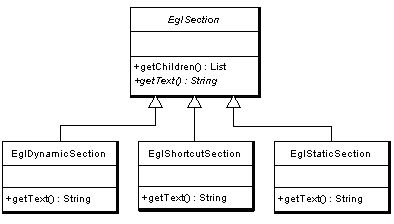
\includegraphics[scale=0.80]{images/EglAbstractSyntax.png}
  \end{center}
  \caption{The abstract syntax of EGL's core.}
  \label{fig:abstractsyntax}
\end{figure}

In common with other template-based code generators, EGL defines
\emph{sections}, from which templates may be constructed. Static
sections delimit sections whose contents appear verbatim in the
generated text. Dynamic sections contain executable code that can be
used to control the generated text.

In its dynamic sections, EGL re-uses EOL's mechanisms for structuring
program control flow, performing model inspection and navigation, and
defining custom operations.  EGL provides an EOL object, \verb|out|,
for use within dynamic sections.  This can be used to perform
operations on the generated text, such as appending and removing
strings and specifying the type of text to be generated.

EGL also provides syntax for defining \textit{dynamic output}
sections, which provide a convenient shorthand for outputting text
from within dynamic sections. Similar syntax is often provided by
template-based code generators.

\section{Concrete Syntax}
\label{concretesyntax}

The concrete syntax of EGL mirrors the style of other
template-based code generation languages. The tag pair \verb|[% %]| is
used to delimit a dynamic section. Any text not enclosed in such a tag
pair is contained in a static section. Listing
\ref{lst:basic} illustrates the use of dynamic and static sections to
form a basic EGL template.

\begin{lstlisting}[basicstyle=\ttfamily\footnotesize, tabsize=2, flexiblecolumns=true, caption=A basic EGL template., label=lst:basic]
[% for (i in Sequence{1..5}) { %]
i is [%=i%]
[% } %]
\end{lstlisting}

The \emph{[\%=expr\%]} construct is shorthand for \emph{[\%
  out.print(expr); \%]}, which appends \emph{expr} to the output
generated by the transformation. Note that the \verb|out| keyword also
provides \emph{println(Object)} and \emph{chop(Integer)} methods, which
can be used to construct text with linefeeds, and to remove the
specified number of characters from the end of the generated text.

EGL exploits EOL's model querying capabilities to output text from
models specified as input to transformations. For example, the EGL
template depicted in Listing \ref{lst:oo} may be used to generate text
from a model that conforms to a metamodel that describes an
object-oriented system.

\begin{lstlisting}[basicstyle=\ttfamily\footnotesize, tabsize=2, flexiblecolumns=true, caption=Generating the name of each Class contained in an input model., label=lst:oo]
[% for (class in Class.allInstances) { %]
[%=class.name%]
[% } %]
\end{lstlisting}

\section{Parsing and Preprocessing}
EGL provides a parser which generates an abstract syntax tree comprising static, dynamic and dynamic output nodes for a given template. A preprocessor then translates each section into corresponding EOL: static and dynamic output sections generate \verb|out.print()| statements. Dynamic sections are already specified in EOL, and require no translation.

Consider the EGL depicted in Listing \ref{lst:basic}.  The
preprocessor produces the EOL
shown in Listing
\ref{lst:preprocessor-eol} -- the \verb|[% %]| and \verb|[%=  %]| tag pairs have been removed, and the text to be output is translated into \verb|out.print()| statements.

\begin{lstlisting}[basicstyle=\ttfamily\footnotesize, tabsize=2, flexiblecolumns=true, caption=Resulting EOL generated by the preprocessor., label=lst:preprocessor-eol]
for (i in Sequence{1..5}) {
   out.print(`i is ');
   out.print(i);
   out.print(`\r\n');
}
\end{lstlisting}

When comparing Listings \ref{lst:basic} and \ref{lst:preprocessor-eol}, it can be seen that the template-based syntax is more concise, while the preprocessed syntax is arguably more readable. For templates where there is more dynamic than static text, such as the one depicted in Listing \ref{lst:basic}, a template-based syntax is often less readable. However, this loss of readability is somewhat mitigated by EGL's developer tools, which are discussed in Section \ref{Tool Support}. By contrast, for templates that exhibit more static than dynamic text, a template-based syntax is often more readable than its preprocessed equivalent.

\section{Deriving EGL from EOL}

In designing functionality specific to M2T transformation, one option
was to 
enrich the existing EOL syntax with  keywords such as \emph{print}, \emph{contentType} 
and \emph{merge}.  However, EOL underpins all Epsilon
languages, and the additional keywords were needed only for M2T.
Furthermore, the refactorings needed to support the new keywords
affect many components -- the lexer, parser, execution context and
execution engine -- complicating maintenance and use by other developers.
Instead, we define a minimal syntax for EGL, allowing easy
implementation of an EGL execution engine as a simple preprocessor for EOL. 
 

The EGL execution engine augments the default context used by EOL
during execution with two read-only, global variables: \emph{out}
(Section \ref{concretesyntax}) and \emph{TemplateFactory} (Section
\ref{Co-ordination}). The \emph{out} object defines methods for
performing operations specific to M2T translation, and the
\emph{TemplateFactory} object provides methods for loading other
templates. The implementation for the latter was extended, late in the
EGL development, to provide support for accessing templates from a
file-system -- a trivial extension that caused no migration problems
for existing EGL templates, due to the way in which EGL extends EOL.

\section{Co-ordination}
\label{Co-ordination}
In the large, M2T transformations need to be able to not only generate
text, but also files, which are then used downstream as development
artefacts.  An M2T tool must provide the language constructs for
producing files and manipulating the local file system.  Often, this
requires that the destination, as well as the contents, be dynamically
defined at a transformation's execution time.

The EGL co-ordination engine supplies mechanisms for generating text
directly to files.  The design encourages decoupling of generated text
from output destinations. The \emph{Template} data-type is provided to
allow nested execution of M2T transformations, and operations on
instances of this data-type facilitate the generation of text directly
to file. A factory object, \emph{TemplateFactory}, is provided to
simplify the creation of \emph{Template} objects.  In Listing
\ref{lst:co-ordination}, these objects are used in an EGL template
that loads the the EGL template in Listing \ref{lst:oo} from the file,
ClassNames.egl, and writes out to disk the text generated by executing
ClassNames.egl.

\begin{lstlisting}[basicstyle=\ttfamily\footnotesize, tabsize=2, flexiblecolumns=true, caption=Storing the name of each Class to disk., label=lst:co-ordination]
[%
  var t : Template := TemplateFactory.load(`ClassNames.egl');
  t.process();
  t.generate(`Output.txt');
%]
\end{lstlisting}

This approach to co-ordination allows EGL to be used to generate one
or more files from a single input model. Moreover, EGL's co-ordination
engine facilitates the specification of platform-specific details (the
destination of any files being generated) separately from the
platform-independent details (the contents of any files being
generated).

\section{Merge Engine}
EGL provides language constructs that allow M2T transformations to
designate regions of generated text as \textit{protected}. The
contents of protected regions are preserved every time a M2T
transformation generates text to the same destination.

Protected regions are specified by the \emph{preserve(String, String,
  String, Boolean, String)} method on the \verb|out| keyword. The first two parameters define the comment delimiters
of the target language. The other parameters provide the name,
enable-state and content of the protected region, as
illustrated in Listing \ref{lst:preserve}.

\begin{lstlisting}[basicstyle=\ttfamily\footnotesize, tabsize=2, flexiblecolumns=true, caption=Protected region declaration using the preserve method., label=lst:preserve]
[%=out.preserve(`/*', `*/', `anId', true,
                `System.out.println(foo);')
%]
\end{lstlisting}

A protected region declaration may have many lines, and use many EGL
variables in the contents definition.  To enhance readability, EGL
provides two additional methods on the \verb|out| keyword:
\emph{startPreserve(String, String, String, Boolean)} and
\verb|stopPreserve|.  Listing \ref{lst:startpreserve} uses these to
generate a protected region equivalent to that in Listing
\ref{lst:preserve}.

\begin{lstlisting}[basicstyle=\ttfamily\footnotesize, tabsize=2, flexiblecolumns=true, caption=Protected region declaration., label=lst:startpreserve]
[%=out.startPreserve(`/*', `*/', `anId', true)%]
System.out.println(foo);
[%=out.stopPreserve()%]
\end{lstlisting}

Because an EGL template may contain many protected regions, EGL also
provides a separate method to set the target language generated by the
current template, \emph{setContentType(String)}. By default, EGL recognises Java, HTML, Visual Basic,
Perl and EGL as valid content types. An alternative configuration file
can be used to specify further content
types. Following a call to \verb|setContentType|, the first two
arguments to the \verb|preserve| and \verb|startPreserve| methods can
be omitted, as shown in Listing \ref{lst:contenttype}.

\begin{lstlisting}[basicstyle=\ttfamily\footnotesize, tabsize=2, flexiblecolumns=true, caption=Setting the content type., label=lst:contenttype]
[% out.setContentType(`Java'); %]
[%=out.preserve(`anId', true, `System.out.println(foo);')%]
\end{lstlisting}

Because some languages define more than one style of comment
delimiter, EGL allows mixed use of  the styles for \verb|preserve| and
\verb|startPreserve| methods.

Once a content type has been specified, a protected region may be declared entirely from a static section, using the syntax  in Listing \ref{lst:manualpr}.

\begin{lstlisting}[basicstyle=\ttfamily\footnotesize, tabsize=2, flexiblecolumns=true, caption=Declaring a protected region from within a static section., label=lst:manualpr]
[% out.setContentType(`Java'); %]
// protected region anId [on|off] begin
System.out.println(foo);
// protected region anId end
\end{lstlisting}

When a template that defines one or more protected regions is
processed by the EGL execution engine, the target output destinations
are interrogated and existing contents of any protected regions are
preserved. If either the output generated by from the template or the
existing contents of the target output destination contains protected
regions, a merging process is invoked. Table \ref{tab:merging} shows
the default behaviour of EGL's merge engine.

\begin{table}[htbp]
  \begin{center}
  \begin{tabular}{|l|l|l|}
  \hline
  \multicolumn{2}{|l|}{\textbf{Protected Region Status}} & \multirow{2}{*}{\textbf{Contents taken from}} \\
  \textbf{Generated} & \textbf{Existing} & \\
  \hline
  On & On     & Existing  \\
  On & Off    & Generated \\
  On & Absent & Generated \\
  \hline
  Off & On     & Existing  \\
  Off & Off    & Generated \\
  Off & Absent & Generated \\
  \hline
  Absent & On  & Neither (causes a warning) \\
  Absent & Off & Neither (causes a warning) \\
  \hline
  \end{tabular}
  \end{center}
\caption{EGL's default merging behaviour.}
\label{tab:merging}
\end{table}

\section{Readability and traceability} 
Conscientious developers apply various \emph{conventions} to produce
readable code.  EGL encourages template developers to prioritise the
readability of templates over the text that they generate. EGL provides a number of text post-processors -- or
\textit{beautifiers} -- that can be executed on output of
transformations to improve readability.  Currently, beautifiers are
invoked via Epsilon's extensions to Apache Ant, an
XML-based build tool for Java.

EGL also provides a traceability API, as a debugging aid, and to
support auditing of the M2T transformation process.  This API
facilitates exploration of the templates executed, files affected and
protected regions processed during a transformation.  Figure
\ref{fig:traceability} shows sample output from the traceability API
after execution of an EGL M2T transformation to generate Java
code from an instance of an OO metamodel.

The beautification interface is minimal, in order to allow re-use of existing 
code formatting algorithms. Consequently, there is presently no traceability support 
for beautified text. However, due to the coarse-grained approach employed by 
EGL's traceability API, this has little impact: Clicking on a beautified protected 
region in the traceability view might not highlight the correct line in the editor.

\begin{figure}[htbp]
  \begin{center}
    \leavevmode
    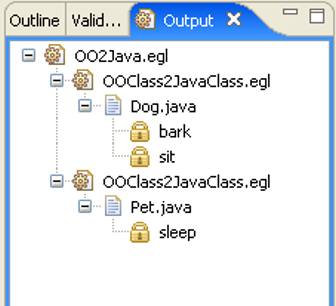
\includegraphics[scale=0.6]{images/TraceView}
  \end{center}
  \caption{Sample output from the traceability API.}
  \label{fig:traceability}
\end{figure}

\subsection{Tool Support}
\label{Tool Support}
The Epsilon platform provides development tools for the Eclipse
development environment. Re-use of Eclipse APIs allows
Epsilon's development tooling to incorporate a large number of
features with minimal effort. Furthermore, the flexibility of the
plug-in architecture of Eclipse enhances modular authoring of
development tools for Epsilon.

In addition to the traceability view shown in Figure
\ref{fig:traceability}, EGL includes an Eclipse editor and an outline
view. In order to aid template readability, these tools provide syntax 
highlighting and a structural overview for EGL templates, respectively. Through its 
integration in the Epsilon perspective, EGL provides an Eclipse workbench 
configuration that is tailored for use with Epsilon's development tools.

%\begin{figure}[htbp]
%  \begin{center}
%    \leavevmode
%    \includegraphics[scale=0.66]{EglWorkspace.png}
%  \end{center}
%  \caption{The EGL editor and outline view.}
%  \label{fig:editorandview}
%\end{figure}

EGL, like other Epsilon languages, provides an Apache ANT
task definition, to facilitate invocation of model-management activies
from within a build script.

\chapter{The Epsilon Comparison Language (ECL)}
\label{sec:ECL}

Model comparison is the task of identifying \emph{matching} elements between models. In general, \emph{matching} elements are elements that are involved in a relationship of interest. For example, before merging homogeneous models, it is essential to identify overlapping (common) elements so that they do not appear in duplicate in the merged model. Similarly, in heterogeneous model merging, it is a prerequisite to identify the elements on which the two models will be merged. Finally, in transformation testing, matching elements are pairs consisting of elements in the input model and their generated counterparts in the output model.

The aim of the Epsilon Comparison Language (ECL) is to enable users to specify comparison algorithms in a rule-based manner to identify pairs of matching elements between two models of potentially different metamodels and modelling technologies. In this section, the abstract and concrete syntax, as well as the execution semantics of the language, are discussed in detail.

%A comparison algorithm separates the model elements of the involved models into two categories: those that have matching elements in the opposite model and those that do not. Moreover, as the algorithm does not necessarily attempt to find matching elements for all the model elements of the involved models, the classification can be further refined to the following:
%
%\begin{enumerate}
%	\item Elements for which matching elements exist in the opposite model
%	\item Elements for which matching elements do not exist in the opposite model
%	\begin{enumerate}
%	\item Elements for which matching has been attempted but no matching elements has been found
%	\item Elements for which no matching has been attempted
%	\end{enumerate}
%\end{enumerate}

\section{Abstract Syntax}

In ECL, comparison specifications are organized in modules (\emph{EcLModule}). As illustrated in Figure \ref{fig:ECL}, EclModule extends EOLLibraryModule which means that it can contain user-defined operations and import other library modules and ECL modules. Apart from operations, an ECL module contains a set of match-rules (\emph{MatchRule}) and a set of \emph{pre} and \emph{post} blocks.

\emph{MatchRules} enable users to perform comparison of model elements at a high level of abstraction. Each match-rule declares a name, and two parameters (\emph{leftParameter} and \emph{rightParameter}) that specify the types of elements it can compare. It also optionally defines a number of rules it inherits (\emph{extends}) and if it is \emph{abstract}, \emph{lazy} and/or \emph{greedy}. The semantics of the latter are discussed shortly.

\begin{landscape}
\begin{figure}
	\centering
		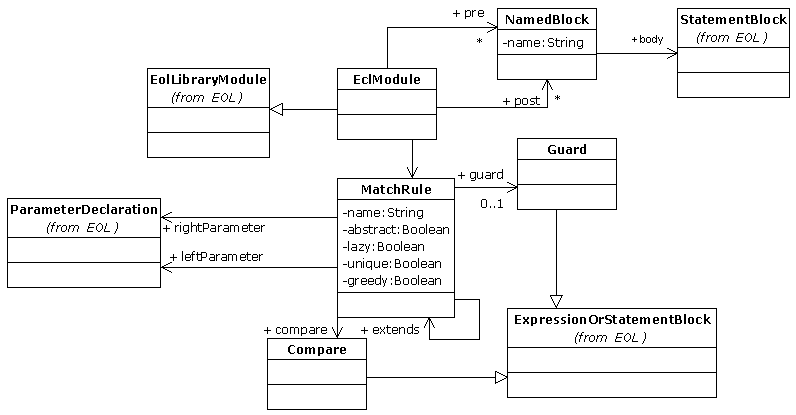
\includegraphics{images/EclAbstractSyntax.png}
	\caption{ECL Abstract Syntax}
	\label{fig:ECL}
\end{figure}
\end{landscape}

A match rule has three parts. The \emph{guard} part is an EOL expression or statement block that further limits the applicability of the rule to an even narrower range of elements than that specified by the \emph{left} and \emph{right} parameters. The \emph{compare} part is an EOL expression or statement block that is responsible for comparing a pair of elements and deciding if they match or not. Finally, the \emph{do} part is an EOL expression or block that is executed if the \emph{compare} part returns true to perform any additional actions required.

\emph{Pre} and \emph{Post} blocks are named blocks of EOL statements which as discussed in the sequel are executed before and after the match-rules have been executed respectively.

\section{Concrete Syntax}

The concrete syntax of a match-rule is displayed in Listing \ref{lst:MatchRuleConcreteSyntax}.

\begin{lstlisting}[basicstyle=\ttfamily\footnotesize, flexiblecolumns=true, numbers=none, nolol=true, caption=Concrete Syntax of a MatchRule, label=lst:MatchRuleConcreteSyntax, language=ECL, numbers=left, tabsize=2]

(@lazy)?
(@greedy)?
(@abstract)? 
rule <name> 
	match <leftParameterName>:<leftParameterType>
	with <rightParameterName>:<rightParameterType>
	(extends (<ruleName>,)*<ruleName>)? {
	
	(guard (:expression)|({statementBlock}))?
	
	compare (:expression)|({statementBlock})
	
	(do {statementBlock})?
	
}
\end{lstlisting}

\emph{Pre} and \emph{post} blocks have a simple syntax that, as presented in Listing \ref{lst:EclPrePostConcreteSyntax}, consists of the identifier (\emph{pre} or \emph{post}), an optional name and the set of statements to be executed enclosed in curly braces.

\begin{lstlisting}[basicstyle=\ttfamily\footnotesize, flexiblecolumns=true, numbers=none, nolol=true, caption=Concrete Syntax of Pre and Post blocks, label=lst:EclPrePostConcreteSyntax, language=ECL, numbers=left, tabsize=2]
(pre|post) <name> {
	statement+
}
\end{lstlisting}

\section{Execution Semantics}

\subsection{Rule and Block Overriding}

An ECL module can import a number of other ECL modules. In such a case, the importing ECL module inherits all the rules and pre/post blocks specified in the modules it imports (recursively). If the module specifies a rule or a pre/post block with the same name, the local rule/block overrides the imported one respectively.

\subsection{Comparison Outcome}

As illustrated in Figure \ref{fig:ECLRuntime}, the result of comparing two models with ECL is a trace (\emph{MatchTrace}) that consists of a number of matches (\emph{Match}). Each match holds a reference to the objects from the two models that have been compared (\emph{left} and \emph{right}), a boolean value that indicates if they have been found to be \emph{matching} or not, a reference to the \emph{rule} that has made the decision, and a Map (\emph{info}) that is used to hold any additional information required by the user. During the matching process, a second, temporary, match trace is also used to detect and resolve cyclic invocation of match-rules as discussed in the sequel.

\begin{figure}
	\centering
		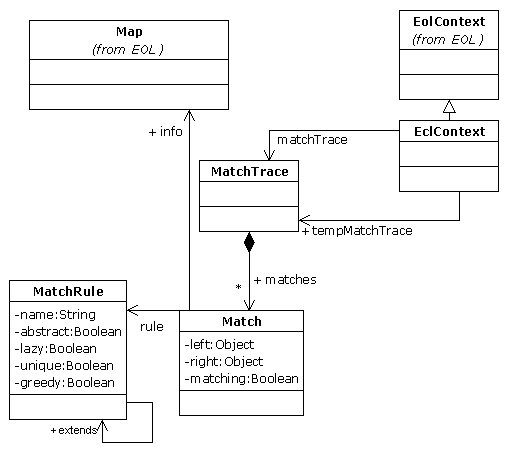
\includegraphics{images/ECLRuntime.png}
	\caption{ECL Match Trace}
	\label{fig:ECLRuntime}
\end{figure}

\subsection{Rule Execution Scheduling}

Non-abstract, non-lazy match-rules are evaluated automatically by the execution engine in a top-down fashion - with respect to their order of appearance - in two passes. In the first pass, each rule is evaluated for all the pairs of instances in the two models that have a type-of relationship with the types specified by the \emph{leftParameter} and \emph{rightParameter} of the rule. In the second pass, each rule that is marked as \emph{greedy} is executed for all pairs that have not been compared in the first pass, and which have a kind-of relationship with the types specified by the rule. In both passes, to evaluate the compare part of the rule, the guard must be satisfied.

Before the compare part of a rule is executed, the compare parts of all of the rules it extends (super-rules) must be executed (recursively). Before executing the compare part of a super-rule, the engine verifies that the super-rule is actually applicable to the elements under comparison by checking for type conformance and evaluating the guard part of the super-rule.

If the compare part of a rule evaluates to true, the optional do part is executed. In the do part the user can specify any actions that need to be performed for the identified matching elements, such as to populate the \emph{info} map of the established \emph{match} with additional information. Finally, a new match is added to the match trace that has its \emph{matching} property set to the logical conjunction of the results of the evaluation of the compare parts of the rule and its super-rules.

\subsection{The \emph{matches()} built-in operation}

To refrain from performing duplicate comparisons and to de-couple match-rules from each other, ECL provides the built-in \emph{matches(opposite : Any)} operation for model elements and collections. When the \emph{matches()} operation is invoked on a pair of objects, it queries the main and temporary match-traces to discover if the two elements have already been matched and if so it returns the cached result of the comparison. Otherwise, it attempts to find an appropriate match rule to compare the two elements and if such a rule is found, it returns the result of the comparison, otherwise it returns false. Unlike the top-level execution scheme, the \emph{matches()} operation invokes both \emph{lazy} and \emph{non-lazy} rules.

In addition to objects, the \emph{matches} operations can also be invoked to match pairs of collections of the same type (e.g. a Sequence against a Sequence). When invoked on ordered collections (i.e. \emph{Sequence} and \emph{OrderedSet}), it examines if the collections have the same size and each item of the source collection matches with the item of the same index in the target collection. Finally, when invoked on unordered collections (i.e. \emph{Bag} and \emph{Set}), it examines if for each item in the source collection, there is a matching item in the target collection irrespective of its index. Users can also override the built-in \emph{matches} operation using user-defined operations with the same name, as discussed in Section \ref{sec:Design.EOL.FeatureNavigation}, that loosen or strengthen the built-in semantics.

\subsection{Cyclic invocation of \emph{matches()}}

Providing the built-in \emph{matches} operation significantly simplifies comparison specifications. It also enhances decoupling between match-rules from each other as when a rule needs to compare two elements that are outside its scope, it does not need to know/specify which other rule can compare those elements explicitly.

On the other hand, it is possible - and quite common indeed - for two rules to implicitly invoke each other. For example consider the match rule of Listing \ref{lst:Tree2Tree} that attempts to match nodes of the simple Tree metamodel displayed in Figure \ref{fig:Tree}.

\begin{figure}
	\centering
		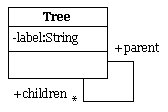
\includegraphics{images/metamodels/Tree.png}
	\caption{The Tree Metamodel}
	\label{fig:Tree}
\end{figure}

\begin{lstlisting}[basicstyle=\ttfamily\footnotesize, flexiblecolumns=true, numbers=none, nolol=true, caption=The Tree2Tree rule, label=lst:Tree2Tree, language=ECL, numbers=left, tabsize=2]
rule Tree2Tree 
	match l : T1!Tree
	with r : T2!Tree {
	
	compare : l.label = r.label and 
		l.parent.matches(r.parent) and
		l.children.matches(r.children)
}
\end{lstlisting}

The rule specifies that for two Tree nodes (\emph{l} and \emph{r}) to match, they should have the same label, belong to matching parents and have matching children. In the absence of a dedicated mechanism for cycle detection and resolution, the rule would end up in an infinite loop. To address this problem, ECL provides a temporary match-trace which is used to detect and resolve cyclic invocations of the \emph{match()} built-in operation.

As discussed above, a match is added to the primary match-trace as soon as the compare part of the rule has been executed to completion. By contrast, a temporary match (with its \emph{matching} property set to \emph{true}) is added to the temporary trace before the compare part is executed. In this way, any subsequent attempts to match the two elements from invoked rules will not re-invoke the rule. Finally, when a top-level rule returns, the temporary match trace is reset.

\section{Fuzzy and Dictionary-based String Matching}
\label{sec:FuzzyComparison}

In the example of Listing \ref{lst:Tree2Tree}, the rule specifies that to match, two trees must - among other criteria - have the same label. However, there are cases when a less-strict approach to matching string properties of model elements is desired. For instance, when comparing two UML models originating from different organizations, it is common to encounter ontologically equivalent classes which however have different names (e.g. Client and Customer). In this case, to achieve a more sound matching, the use of a dictionary or a lexical database (e.g. WordNet \cite{Wordnet}) is necessary. Alternatively, fuzzy string matching algorithms such as those presented in \cite{FuzzyStringMatching} can be used.

As several such tools and algorithms have been implemented in various programming languages, it is a sensible approach to reuse them instead of re-implementing them. For example, in Listing \ref{lst:FuzzyTree2Tree} a wrapper for the Simmetrics \cite{Simmetrics} fuzzy string comparison tool is used to compare the labels of the trees using the Levenshtein \cite{Levenshtein} algorithm. To achieve this, line 11 invokes the \emph{fuzzyMatch()} operation defined in lines 16-18 which uses the simmterics native tool (instantiated in lines 2-4) to match the two labels using their Levenshtein distance with a threshold of 0.5.

\begin{lstlisting}[basicstyle=\ttfamily\footnotesize, flexiblecolumns=true, numbers=none, nolol=true, caption=The FuzzyTree2Tree rule, label=lst:FuzzyTree2Tree, language=ECL, numbers=left, tabsize=2]
pre {
	var simmetrics = 
		new Native("org.epsilon.ecl.tools.
			textcomparison.simmetrics.SimMetricsTool"); 
}

rule FuzzyTree2Tree 
	match l : T1!Tree
	with r : T2!Tree {
	
	compare : l.label.fuzzyMatch(r.label) and 
		l.parent.matches(r.parent) and
		l.children.matches(r.children)
}

operation String fuzzyMatch(other : String) : Boolean {
	return simmetrics.similarity(self,other,"Levenshtein") > 0.5;
}\end{lstlisting}

\section{Interactive Matching}
\label{sec:InteractiveModelComparison}

Using the user interaction features discussed in Section \ref{sec:Design.EOL.UserInput} the comparison can become interactive by replacing the \emph{fuzzyMatch} operation of listing \ref{lst:FuzzyTree2Tree} with the one specified in Listing \ref{lst:InteractiveTree2TreeComparison}. The fuzzyMatch operation of Listing \ref{lst:InteractiveTree2TreeComparison}, performs the fuzzy string comparison and -- as the previous version -- if the result is greater than 0.5 it returns true. However, in this updated version if the result is lower than 0.5 but greater than 0.3, it prompts the user to confirm if the two strings match, and if it is lower than 0.3 it returns false.

\begin{lstlisting}[basicstyle=\ttfamily\footnotesize, flexiblecolumns=true, numbers=none, nolol=true, caption=An interactive version of the fuzzyMatch operation of Listing \ref{lst:FuzzyTree2Tree}, label=lst:InteractiveTree2TreeComparison, language=ECL, numbers=left, tabsize=2]
operation String fuzzyMatch(other : String) : Boolean {
	var similarity : Real;
	similarity = simmetrics.similarity(self,other,"Levenshtein");
	if (similarity > 0.5) {
		return true;
	}
	else if (similarity > 0.3) {
		return UserInput.confirm(self + " matches " + other + "?");
	}
	else {
		return false;
	}
}\end{lstlisting}

\section{Exploiting the Comparison Outcome}

Users can query and modify the match trace calculated during the comparison process in the post sections of the module or export it into another application or Epsilon program. For example, in a post section, the trace can be printed to the default output stream or serialized into a model of an arbitrary metamodel. In another use case, the trace may be exported to be used in the context of a validation module that will use the identified matches to evaluate inter-model constraints, or in a merging module that will use the matches to identify the elements on which the two models will be merged. The topic of interoperability - that includes importing and exporting objects - between modules expressed in different Epsilon languages is discussed in Chapter \ref{chp:Workflow}.

\chapter{The Epsilon Merging Language (EML)}
\label{sec:EML}

The aim of EML is to contribute model merging capabilities to Epsilon. More specifically, EML can be used to merge an arbitrary number of input models of potentially diverse metamodels and modelling technologies. This section provides a discussion on the motivation for implementing EML, its abstract and concrete syntax, as well as its execution semantics. It also provides two examples of merging homogeneous and heterogeneous models.

\section{Motivation}

A mechanism that enables automatically merging models on a set of established correspondences has a number of applications in a model driven engineering process. For instance, it can be used to unify two complementary, but potentially overlapping, models that describe different views of the same system. In another scenario, it can be used to merge a core model with an aspect model (potentially conforming to different metamodels), as discussed in \cite{MDAGuide} where a core \emph{Platform Independent Model (PIM)} is merged with a \emph{Platform Definition Model (PDM)}, that contributes platform-specific aspects, into a \emph{Platform Specific Model (PSM)}.

\subsection{Phases of Model Merging}

Existing research \cite{Pottinger2003,Batini1986} has demonstrated that model merging can be decomposed into four distinct phases: comparison, conformance checking, merging and reconciliation (or restructuring).

\paragraph{Comparison Phase} In the comparison phase, correspondences between equivalent elements of the source models are identified, so that such elements are not propagated in duplicate in the merged model.

%In \cite{ModelWeaver} the ModelWeaver, a generic framework for capturing different types of relationships, such as match relationships, between elements of different models is illustrated.  Matching pairs of elements can be defined graphically through a tree-based user interface and declared relationships can be stored in a separate \textit{weaving model}. Weaving models can be used later by other tools such as model transformation or model merging tools. While this is a flexible approach that promotes reuse, it does not scale well since manual definition of each matching pair is a labour intensive process.

%In \cite{Alanen2003}, matching is performed using persistent model-element identifiers (i.e. using the $xmi.id$ identifier). However, this only applies to comparison of models that are versions of a common ancestor. In \cite{Gray2005}, matching is performed by comparing the \textit{names} of the elements of the two models. Nevertheless, there are model elements that do not have a name (e.g. instances of the $Multiplicity$ UML metaclass) to compare.

\paragraph{Conformance Checking Phase} In this phase, elements that have been identified as matching in the previous phase are examined for conformance with each other. The purpose of this phase is to identify potential conflicts that would render merging infeasible. The majority of proposed approaches, such as \cite{Letkeman2005}, address conformance checking of models complying with the same metamodel. 
 
\paragraph{Merging Phase}
Several approaches have been proposed for the merging phase. In \cite{Pottinger2003,Melnik2003}, graph-based algorithms for merging models of the same metamodel are proposed. In \cite{Letkeman2005}, an interactive process for merging of UML 2.0 models is presented. There are at least two weaknesses in the methods proposed so far. First, they only address the issue of merging models of the same metamodel, and some of them address a specific metamodel indeed. Second, they use an inflexible merging algorithm and do not provide means for extending or customizing its logic.

\paragraph{Reconciliation and Restructuring Phase}
After the merging phase, the target model may contain inconsistencies that need fixing. In the final step of the process, such inconsistencies are removed and the model is \textit{polished} to acquire its final form. Although the need for a reconciliation phase is discussed in \cite{Batini1986,Melnik2003}, in the related literature the subject is not explicitly targeted.

\subsection{Relationship between Model Merging and Model Transformation}

A merging operation is a transformation in a general sense, since it transforms some input (source models) into some output (target models). However, as discussed throughout this section, a model merging facility has special requirements (support for comparison, conformance checking and merging pairs of input elements) that are not required for typical \textit{one-to-one} or \textit{one-to-many} transformations \cite{Czarnecki2003} and are therefore not supported by contemporary model transformation languages.

\section{Realizing a Model Merging Process with Epsilon}

The first two steps of the process described above can be realized with existing languages provided by Epsilon. As discussed in Section \ref{sec:ECL}, the comparison step can be realized with the Epsilon Comparison Language (ECL). Following that, the Epsilon Validation Language (EVL) can be used to validate the identified correspondences using the match trace calculated by ECL. The Epsilon Merging Language (EML) presented below provides support for the last two steps of the process (merging and reconciliation/restructuring).

\section{Abstract Syntax}

In EML, merging specifications are organized in modules (\emph{EmlModule}). As displayed in Figure \ref{fig:EmlAbstractSyntax}, \emph{EmlModule} inherits from \emph{EtlModule}.

\begin{sidewaysfigure}
  \centering
  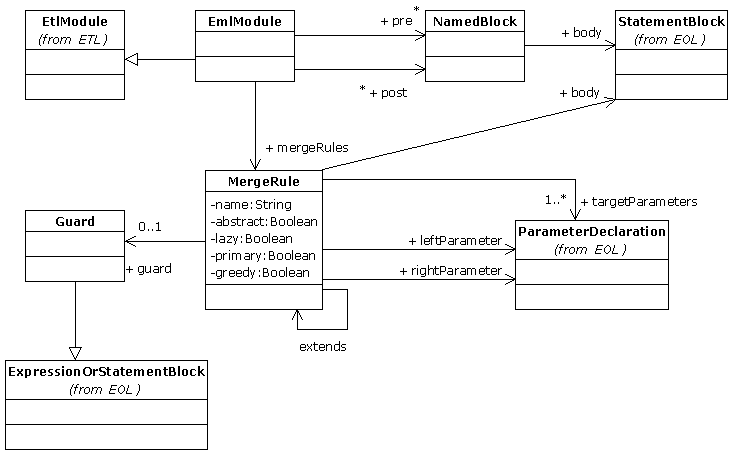
\includegraphics{images/EmlAbstractSyntax.png}
  \caption{The Abstract Syntax of EML}
  \label{fig:EmlAbstractSyntax}
\end{sidewaysfigure}

By extending \emph{EtlModule}, an EML module can contain a number of transformation rules and user-defined operations. An EML module can also contain one or more merge rules as well as a set of \emph{pre} and \emph{post} named EOL statement blocks. As usual, \emph{pre} and \emph{post} blocks will be run before and after all rules, respectively.

Each merge rule defines a name, a left, a right, and one or more target parameters. It can also extend one or more other merge rules and be defined as having one or more of the following properties: abstract, greedy, lazy and primary.

\section{Concrete Syntax}

Listing \ref{lst:EmlConcreteSyntax} demonstrates the concrete syntax of EML merge-rules.

\begin{lstlisting}[float=tbp, caption=Concrete syntax of an EML merge-rule, label=lst:EmlConcreteSyntax, language=EML]
(@abstract)?
(@lazy)?
(@primary)?
(@greedy)?
rule <name>
	merge <leftParameter>
	with <rightParameter>
	into (<targetParameter>(, <targetParameter>)*)?
	(extends <ruleName>(, <ruleName>)*)? {

	statementBlock
	
}
\end{lstlisting}

\emph{Pre} and \emph{post} blocks have a simple syntax that, as presented in Listing \ref{lst:EmlPrePostConcreteSyntax}, consists of the identifier (\emph{pre} or \emph{post}), an optional name and the set of statements to be executed enclosed in curly braces.

\begin{lstlisting}[float=tbp, caption=Concrete Syntax of Pre and Post blocks, label=lst:EmlPrePostConcreteSyntax, language=EML]
(pre|post) <name> {
	statement+
}
\end{lstlisting}

\section{Execution Semantics}

\subsection{Rule and Block Overriding}
An EML module can import a number of other EML and ETL modules. In this case, the importing EML module inherits all the rules and pre/post blocks specified in the modules it imports (recursively). If the module specifies a rule or a pre/post block with the same name, the local rule/block overrides the imported one respectively.

\subsection{Rule Scheduling}
When an EML module is executed, the \emph{pre} blocks are executed in the order in which they have been defined.

Following that, for each \emph{match} of the established \emph{matchTrace} the applicable non-abstract, non-lazy merge rules are executed. When all \emph{matches} have been merged, the transformation rules of the module are executed on all applicable elements - that have not been merged - in the models.

Finally, after all rules have been applied, the \emph{post} blocks of the module are executed.

\subsection{Rule Applicability}
By default, for a merge-rule to apply to a \emph{match}, the \emph{left} and \emph{right} elements of the match must have a \emph{type-of} relationship with the \emph{leftParameter} and \emph{rightParameter} of the rule respectively. This can be relaxed to a \emph{kind-of} relationship by specifying that the merge rule is \emph{greedy} (using the \emph{@greedy} annotation in terms of concrete syntax).

\subsection{Source Elements Resolution}

As with model transformation, in model merging it is often required to resolve the counterparts of an element of a source model into the target models. In EML, this is achieved by overloading the semantics of the \emph{equivalents()} and \emph{equivalent()} operations defined by ETL. In EML, in addition to inspecting the transformation trace and invoking any applicable transformation rules, the \emph{equivalents()} operation also examines the \emph{mergeTrace} (displayed in Figure \ref{fig:EmlRuntime}) that stores the results of the application of merge-rules and invokes any applicable (both lazy and non-lazy) rules.

Similarly to ETL, the order of the results of the \emph{equivalents()} operation respects the order of the (merge or transform) rules that have produced them. An exception to that occurs if one of the rules has been declared as primary, in which case its results are prepended to the list of elements returned by equivalent.

\begin{figure}
	\centering
		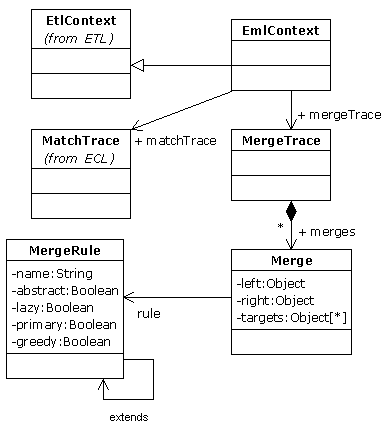
\includegraphics{images/EmlRuntime.png}
	\caption{The EML runtime}
	\label{fig:EmlRuntime}
\end{figure}

\section{Homogeneous Model Merging Example}

In this scenario, two models conforming to the Graph metamodel need to be merged. The first step is to compare the two graphs using the ECL module of Listing \ref{lst:CompareGraph}.

\begin{lstlisting}[float=tbp, caption=ECL module for comparing two instances of the Graph metamodel, label=lst:CompareGraph, language=ECL, tabsize=2]
rule MatchNodes /*@\label{line:MatchNodes}@*/
	match l : Left!Node
	with r : Right!Node {

	compare : l.label = r.label
}

rule MatchEdges /*@\label{line:MatchEdges}@*/
	match l : Left!Edge
	with r : Right!Edge {

	compare : l.source.matches(r.source)
		and l.target.matches(r.target)
}

rule MatchGraphs /*@\label{line:MatchGraphs}@*/
	match l : Left!Graph
	with r : Right!Graph {

	compare : true
}
\end{lstlisting}

The \emph{MatchNodes} rule in line \ref{line:MatchNodes} defines that two nodes match if they have the same label. The \emph{MatchEdges} rule in line \ref{line:MatchEdges} specifies that two edges match if both their source and target nodes match (regardless of whether the labels of the edges match or not as it is assumed that there can not be two distinct edges between the same nodes). Finally, since only one instance of Graph is expected to be in each model, the \emph{MatchGraphs} rule in line \ref{line:MatchGraphs} returns \emph{true} for any pair of Graphs\footnote{Both assumptions can be checked using EVL before matching/merging takes place but this is out of the scope of this example}.

Having established the necessary correspondences between matching elements of the two models, the EML specification of listing \ref{lst:MergeGraphs}.

\begin{lstlisting}[float=tbp, label=lst:MergeGraphs, caption=EML module for merging two instances of the Graph metamodel on the correspondences identified in Listing \ref{lst:CompareGraph} , language=EML]
import "Graphs.etl";

rule MergeGraphs /*@\label{line:MergeGraphs}@*/
	merge l : Left!Graph
	with r : Right!Graph
	into t : Target!Graph {
	
	t.label = l.label + " and " + r.label;
	
}

@abstract
rule MergeGraphElements /*@\label{line:MergeGraphElements}@*/
	merge l : Left!GraphElement
	with r : Right!GraphElement
	into t : Target!GraphElement {
	
	t.graph ::= l.graph;
	
}

rule MergeNodes /*@\label{line:MergeNodes}@*/
	merge l : Left!Node
	with r : Right!Node
	into t : Target!Node 
	extends GraphElements {
	
	t.label = "c_" + l.label;
	
}
rule MergeEdges /*@\label{line:MergeEdges}@*/
	merge l : Left!Edge
	with r : Right!Edge
	into t : Target!Edge 
	extends GraphElements {
	
	t.source ::= l.source;
	t.target ::= l.target;
	
}
\end{lstlisting}

In line \ref{line:MergeGraphs}, the \emph{MergeGraphs} merge rule specifies that two matching Graphs (\emph{l} and \emph{r}) are to be merged into one Graph \emph{t} in the target model that has as a label, the concatenation of the labels of the two input graphs separated using 'and'. The \emph{mergeNodes} rule In line \ref{line:MergeNodes} specifies that two matching Nodes are merged into a single Node in the target model. The label of the merged node is derived by concatenating the c (for common) static string with the label of the source Node from the left model. Similarly, the \emph{MergeEdges} rule specifies that two matching Edges are merged into a single Edge in the target model. The source and target nodes of the merged Edge are set to the equivalents (::=) of the source and target nodes of the edge from the left model.

To reduce duplication, the \emph{MergeNodes} and \emph{MergeEdges} rules extend the abstract \emph{MergeGraphElements} rule specified in line \ref{line:MergeGraphElements} which assigns the \emph{graph} property of the graph element to the equivalent of the left graph.

The rules displayed in Listing \ref{lst:MergeGraphs} address only the matching elements of the two models. To also copy the elements for which no equivalent has been found in the opposite model, the EML module imports the ETL module of Listing \ref{lst:CopyGraph}.

\begin{lstlisting}[float=tbp, caption=The Graphs.etl ETL transformation module, label=lst:CopyGraph, language=ETL]
rule TransformGraph 
	transform s : Source!Graph
	to t : Target!Graph {
	
	t.label = s.label;
	
}

@abstract
rule TransformGraphElement 
	transform s : Source!GraphElement
	to t : Target!GraphElement {
	
	t.graph ::= s.graph;
}

rule TransformNode /*@\label{line:TransformNode}@*/
	transform s : Source!Node
	to t : Target!Node 
	extends TransformGraphElement {
	
	t.label = s.graph.label + "_" + s.label;
}

rule TransformEdge 
	transform s : Source!Edge
	to t : Target!Edge 
	extends TransformGraphElement {
	
	t.source ::= s.source;
	t.target ::= s.target;	
} 
\end{lstlisting}

The rules of the ETL module apply to model elements of both the Left and the Right model as both have been aliased as Source. Of special interest is the TransformNode rule in line \ref{line:TransformNode} that specifies that non-matching nodes in the two input models will be transformed into nodes in the target model the labels of which will be a concatenation of their input graph and the label of their counterparts in the input models.

Executing the ECL and EML modules of Listings \ref{lst:CompareGraph} and \ref{lst:MergeGraphs} on the exemplar models displayed in Figures \ref{fig:LeftGraph} and \ref{fig:RightGraph} creates the target model of Figure \ref{fig:TargetGraph}.

\begin{figure}
	\centering
		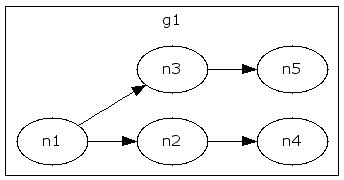
\includegraphics{images/LeftGraph.png}
	\caption{Left input model}
	\label{fig:LeftGraph}
\end{figure}


\begin{figure}
	\centering
		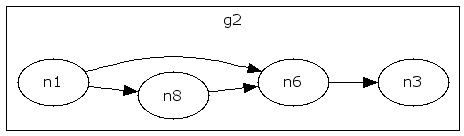
\includegraphics{images/RightGraph.png}
	\caption{Right input model}
	\label{fig:RightGraph}
\end{figure}


\begin{figure}
	\centering
		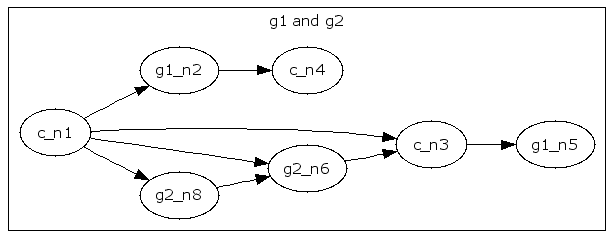
\includegraphics{images/MergedGraph.png}
	\caption{Target model derived by merging the models of Figures \ref{fig:LeftGraph} and \ref{fig:RightGraph}}
	\label{fig:TargetGraph}
\end{figure}

\chapter{Implementing a New Task-Specific Language}
\label{sec:Design.ImplementingANewLanguage}

Although Epsilon already provides languages for a wide range of model management tasks, additional tasks that could benefit from the convenience syntax and dedicated semantics of a task-specific language are likely to be identified in the future. Thus, this section distils the experiences obtained through the construction of existing task-specific languages to provide guidance on how to identify a task for which a dedicated language can be beneficial and develop the respective task-specific language for it atop the infrastructure provided by Epsilon.

\section{Identifying the need for a new language}

The first step of the process of constructing a new task-specific language is to identify a specific task for which a dedicated language is more appropriate than the general-purpose EOL. Typically, recurring syntactic and semantic patterns that emerge when attempting to implement the task using EOL indicate that a new task-specific language may be useful.

For example, before the introduction of the Epsilon Comparison Language, pure EOL was being used to perform model comparison. A simple comparison specification that establishes name-based matches between classes/attributes and tables/columns between two OO and DB models respectively using EOL is demonstrated in Listing \ref{lst:ComparisonEOL}.

Two patterns can be readily detected by inspecting the EOL code in Listing \ref{lst:ComparisonEOL}. First, explicit variables (\emph{matchingCT}, \emph{matchingAT}) are defined to capture the matching elements (class-table and attribute-column)identified during the comparison process. Also, to check all elements of one type (classes against tables and attributes against columns) repeated for statements are used in lines \ref{line:For11}--\ref{line:For12} and \ref{line:For21}--\ref{line:For22}. By contrast, Listing \ref{lst:ComparisonECL} which is specified using the task-specific ECL language does not include such low-level information. Instead it defines only the types of elements that need to be compared and the criteria on which comparison must performed and leaves the mundane tasks of scheduling and maintaining the match trace to the execution engine.

\begin{lstlisting}[caption=Comparing an OO model with a DB model using EOL, label=lst:ComparisonEOL, language=EOL]
var matchingCT : Sequence; /*@\label{line:MatchTrace1}@*/
var matchingAC : Sequence; /*@\label{line:MatchTrace2}@*/
for (c in OO!Class.allInstances) { /*@\label{line:For11}@*/
	for (t in DB!Table.allInstances) { /*@\label{line:For12}@*/
		if (t.name = c.name) {
			matchingCT.add(Sequence{c,t});
			for (att in c.attributes) { /*@\label{line:For21}@*/
				for (col in t.columns) { /*@\label{line:For22}@*/
					if (att.name = c.name) {
						matchingAC.add(Sequence{att, col});
					}
				}
			}
		}
	}
}
\end{lstlisting}

\begin{lstlisting}[caption=Comparing an OO model with a DB model using ECL, label=lst:ComparisonECL, language=ECL]
rule ClassTable
	match c : OO!Class
	with t : DB!Table {
	
	compare : c.name = t.name
}

rule AttributeColumn
	match a : OO!Attribute 
	with c : DB!Column {
	
	compare : a.name = c.name and
		a.class.matches(c.table)
}
\end{lstlisting}

\section{Eliciting higher-level constructs from recurring patterns}

Once recurring patterns, such as those discussed above, have been identified, the next step of the process is to derive higher level constructs from them. For instance, in the previous example, the nested for loops and the explicit trace variable declaration and population have been replaced by task-specific match rules.

Introducing higher-level involves defining its abstract and concrete syntax as well as its connection points with the underlying infrastructure. For example, in the case of ECL, the types of match rules are EOL model element types, the \emph{guard} and \emph{check} parts of a rule are EOL expressions or statements blocks and the \emph{pre} and \emph{post} blocks as well as the \emph{do} part of each rule are blocks of EOL statements.

\section{Implement Execution Semantics and Scheduling}

Once higher-level constructs (e.g. task-specific rules) have been identified and specified, their execution semantics and scheduling must be implemented similarly to what has been done for existing languages. Development of existing languages has demonstrated that task-specific constructs often need to provide more than one modes of execution (e.g. the \emph{lazy} and \emph{greedy} modes of ETL transformation rules discussed in Section \ref{sec:ETL.ExecutionSemantics}). 

A lightweight way to easily provide new execution modes and semantics for rules and user-defined operations without modifying the syntax of the language and introducing new keywords that may conflict with existing code, is through the annotations mechanism provided by EOL (see Section \ref{sec:Design.EOL.Annotations}). This approach has been adopted for the definition a small unit-testing language (EUnit), which is discussed in detail in \cite{EUnit}.

\section{Overriding Semantics}

In certain cases, it is useful to modify the semantics of certain constructs in EOL to meet the purposes of the task-specific language. An example of such a modification occurs in EVL where -- as discussed in Section \ref{sec:Design.EVL.ExecutionSemantics} -- the scope of the variables defined in \emph{guard} expression/block is extended so that variables can be reused in the context of non-nested blocks such as the \emph{title}, and \emph{check} parts of the invariant. Another example of overriding the semantics of EOL is the implementation of the special assignment operator ($::=$) by ETL which was discussed in \ref{sec:Design.ETL.SpecialAssignmentOperator}.






\clearpage
\chapter{Orchestration Workflow}
\label{chp:Workflow}

The previous chapter has provided a detailed discussion on a number of task-specific languages, each one addressing an individual model management task. However, in practice, model management tasks are seldom carried out in isolation; instead, they are often combined together to form complex workflows. Therefore, of similar importance to the existence of individual task-specific management languages is the provision of a mechanism that enables developers to compose modular and reusable tasks into complex automated processes. In a broader context, to facilitate implementation of seamless workflows, an appropriate MDE workflow mechanism should also support mainstream development tasks such as file management, version control management, source code compilation and invocation of external programs and services.

\section{Motivation}
\label{sec:Workflow.Motivation}

As a motivating example, an exemplar workflow that consists of both MDD tasks (1-4, 6) and mainstream software development tasks (5, 7) is displayed below.

\begin{enumerate}
	\item Load a UML model
	\item Validate it
	\item Transform it into a Database Schema model
	\item Generate Java code from the UML model
	\item Compile the Java code
	\item Generate SQL code from the Database model
	\item Deploy the SQL code in a Database Management System (DBMS)
\end{enumerate}

In the above workflow, if the validation step (2) fails, the entire process should be aborted and the identified errors should be reported to the user. This example demonstrates that to be of practical use, a task orchestration framework needs to be able to coordinate both model management and mainstream development tasks and provide mechanisms for establishing dependencies between different tasks. 

This chapter presents such a framework for orchestrating modular model management tasks implemented using languages of the Epsilon platform. As the problem of task coordination is common in software development, many technical solutions have been already proposed and are widely used by software practitioners. In this context, designing a new general-purpose workflow management solution was deemed inappropriate. Therefore, the task orchestration solution discussed here has been designed as an extension to the robust and widely used ANT \cite{ANT} framework. A brief overview of ANT as well as a discussion on the choice to design the orchestration workflow of Epsilon atop it is provided below.

\section{The ANT Tool}
\label{sec:Workflow.ANT}

ANT, named so because it is \textit{a little thing that can be used to build big things} \cite{AntBook}, is a robust and widely-used framework for composing automated workflows from small reusable activities. The most important advantages of ANT, compared to traditional build tools such as \emph{gnumake} \cite{GnuMake}, is that it is platform independent and easily extensible. Platform independence is achieved by building atop Java, and extensibility is realized through a lightweight binding mechanism that enables developers to contribute custom tasks using well defined interfaces and extension points.

Although a number of tools with functionality similar to ANT exist in the Java community, only Maven \cite{Maven} is currently of comparable magnitude in terms of user-basis size and robustness. Outlining the discussion provided in \cite{AntVsMaven}, ANT is considered to be easier to learn and to enable low-level control, while Maven is considered to provide a more elaborate task organization scheme. Nevertheless, the two frameworks are significantly similar and the ANT technical solution discussed in this chapter can easily be ported to work with the latter.

This section provides a brief discussion of the structure and concrete syntax of ANT workflows, as well as the extensibility mechanisms that ANT provides to enable users contribute custom tasks.

\subsection{Structure}
In ANT, each workflow is captured as a \textit{project}. A simplified illustration of the structure of an ANT project is displayed in Figure \ref{fig:AntCore}. Each ANT project consists of a number of \textit{targets}. The one specified as the \emph{default} is executed automatically when the project is executed. Each \emph{target} contains a number of \emph{tasks} and \emph{depends} on other targets that must be executed before it. An ANT task is responsible for a distinct activity and can either succeed or fail. Exemplar activities implemented by ANT tasks include file system management, compiler invocation, version management and remote artefact deployment.

\begin{figure}
	\centering
		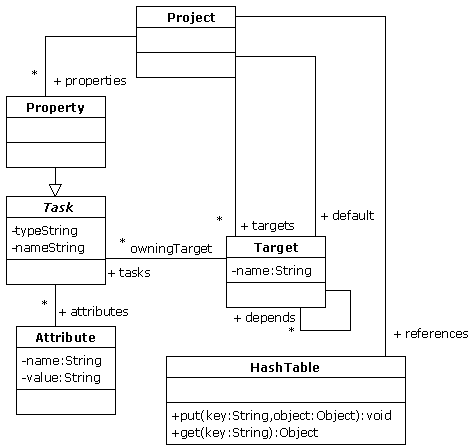
\includegraphics{images/AntCore.png}
	\caption{Simplified ANT object model}
	\label{fig:AntCore}
\end{figure}

\subsection{Concrete Syntax}

In terms of concrete syntax, ANT provides an XML-based syntax. In Listing \ref{lst:ANTExample}, an exemplar ANT project that compiles a set of Java files is illustrated. The project contains one target (\emph{main}) which is also set to be the \emph{default} target. The \emph{main} target contains one \emph{javac} task that specifies attributes such as \emph{srcdir}, \emph{destdir} and \emph{classpath}, which define that the Java compiler will compile a set of Java files contained into the \emph{src} directory into classes that should be placed in the \emph{buiild} directory using \emph{dependencies.jar} as an external library.

\begin{lstlisting}[caption=Compiling Java classes using the javac task, label=lst:ANTExample]
<project default="main">
	<target name="main"/>
	  <javac srcdir="${src}"
	         destdir="${build}"
	         classpath="dependencies.jar"
	         debug="on"
	         source="1.4"/>
	</target>
</project>
\end{lstlisting}

\subsection{Extending ANT}

Binding between the XML tags that describe the tasks and the actual implementations of the tasks is achieved through a light-weight mechanism at two levels. First, the tag (in the example of Listing \ref{lst:ANTExample}, \emph{javac}) is resolved to a Java class that extends the \emph{org.apache.ant.Task} abstract class (in the case of \emph{javac}, the class is \emph{org.apache.tools.ant.taskdefs.Javac}) via a configuration file. Then, the attributes of the tasks (e.g. \emph{srcdir}) are set using the reflective features that Java provides. Finally, the \emph{execute()} method of the task is invoked to perform the actual job.

This lightweight and straightforward way of defining tasks has rendered ANT particularly popular in the Java development community and currently there is a large number of tasks contributed by ANT users \cite{AntExternalTasks}, ranging from invoking tools such as code generators and XSLT processors, to emulating logical control flow structures such as \emph{if} conditions and \emph{while} loops. The AMMA platform \cite{AMMA} also provides integration of model driven engineering tools such as TCS \cite{TCS} and ATL \cite{ATL} with ANT.

ANT also supports more advanced features including nested XML elements and \emph{filesets}, however providing a complete discussion is beyond the scope of this paper. For a definitive guide to ANT readers can refer to \cite{AntBook}.

\section{Integration Challenges}
\label{sec:Workflow.IntegrationChallenges}

A simple approach to extending ANT with support for model management tasks would be to implement one standalone task for each language in Epsilon. However, such an approach demonstrates a number of integration and performance shortcomings which are discussed below. 

Since models are typically serialized in the file system, before a task is executed, the models it needs to access/modify must be parsed and loaded in memory. In the absence of a more elaborate framework, each model management task would have to take responsibility for loading and storing the models it operates on. Also, in most workflows, more than one task operates on the same models sequentially, and needlessly loading/storing the same models many times in the context of the same workflow is an expensive operation both time and memory-wise, particularly as the size of models increases.

Another weakness of this primitive approach is limited inter-task communication. In the absence of a communication framework that allows model management tasks to exchange information with each other, it is often the case that many tasks end up performing the same (potentially expensive) queries on models. By contrast, an inter-task communication framework would enable time and resource intensive calculations to be performed once and their results to be communicated to all interested subsequent tasks.

Having discussed ANT, Epsilon and the challenges their integration poses, the following sections presents the design of a solution that enables developers to invoke model management tasks in the context of ANT workflows. The solution consists of a core framework that addresses the challenges discussed in Section \ref{sec:Workflow.IntegrationChallenges}, a set of specific tasks, each of which implements a distinct model management activity, and a set of tasks that enable developers to initiate and manage transactions on models using the respective facilities provided by the model connectivity layer discussed in Section \ref{sec:EMC.ModelTransactionSupport}. 

\section{Framework Design and Core Tasks}
\label{sec:Workflow.Framework}

The role of the core framework, illustrated in Figure \ref{fig:Core}, is to provide model loading and storing facilities as well as runtime communication facilities to the individual model management tasks that build atop it. This section provides a detailed discussion of the components it consists of.

\begin{landscape}
\begin{figure}
	\centering
		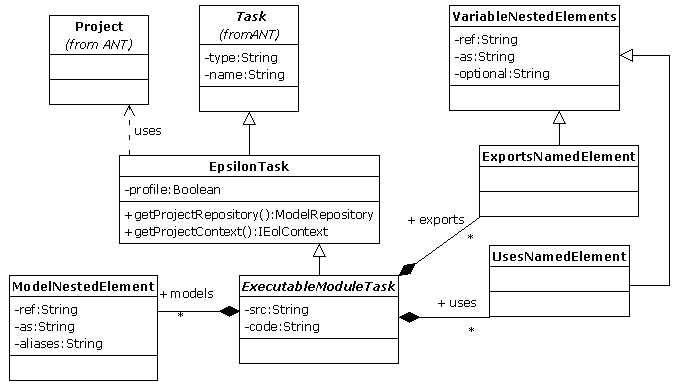
\includegraphics{images/AntEpsilon.png}
	\caption{Core Framework}
	\label{fig:Core}
\end{figure}
\end{landscape}

\begin{figure}
	\centering
		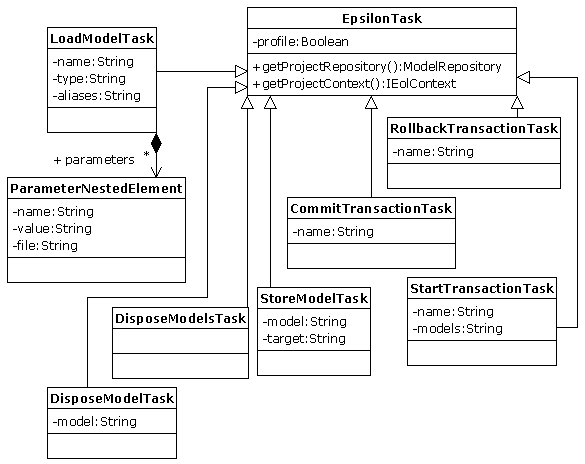
\includegraphics{images/AntEpsilonModels.png}
	\caption{Core Models Framework}
	\label{fig:CoreModels}
\end{figure}

\subsection{The EpsilonTask task}
An ANT task can access the project in which it is contained by invoking the \emph{Task.getProject()} method. To facilitate sharing of arbitrary information between tasks, ANT projects provide two convenience methods, namely \emph{addReference(String key, Object ref)} and \emph{getReference(String key) : Object}. The former is used to add key-value pairs, which are then accessible using the latter from other tasks of the project.

To avoid loading models multiple times and to enable on-the-fly management of models from different Epsilon modules without needing to store and re-load the models after each task, a reference to a project-wide model repository has been added to the current ANT project using the \emph{addReference} method discussed above. In this way, all the subclasses of the abstract \emph{EpsilonTask} can invoke the \emph{getProjectRepository()} method to access the project model repository. 

Also, to support a variable sharing mechanism that enables inter-task communication, the same technique has been employed; a shared context, accessible by all Epsilon tasks via the \emph{getProjectContext()} method, has been added. Through this mechanism, model management tasks can export variables to the project context (e.g. traces or lists containing results of expensive queries) which other tasks can then reuse.

\emph{EpsilonTask} also specifies a \emph{profile} attribute that defines if the execution of the task must be profiled using the profiling features provided by Epsilon. Profiling is a particularly important aspect of workflow execution, especially where model management languages are involved. The main reason is that model management languages tend to provide convenient features which can however be computationally expensive (such as the \emph{allInstances()} EOL built-in feature that returns all the instances of a specific metaclass in the model) and when used more often than really needed, can significantly degrade the overall performance.

%\subsection{Tasks for Loading and Storing Models}

\subsection{Model Loading Task}

The \textit{LoadModelTask (epsilon.loadModel)} loads a model from an arbitrary location (e.g. file-system, database) and adds it to the project repository so that subsequent Epsilon tasks can query or modify it. Since Epsilon supports many modelling technologies (e.g. EMF, MDR, XML), the \textit{LoadModelTask} defines only three generic attributes. The \textit{name} attribute specifies the name of the model in the project repository. The \textit{type} attribute specifies the modelling technology with which the model is captured and is used to resolve the technology-specific model loading functionality. Finally, the \textit{aliases} attribute defines a comma-separated list of alternative names by which the model can be accessed in the model repository.

The rest of the information needed to load a model is implementation-specific and is therefore provided through \textit{parameter} nested elements, each one defining a pair of \textit{name}-\textit{value} attributes. As an example, a task for loading an EMF model that has a file-based ECore metamodel is displayed in Listing \ref{lst:LoadModelTask}.

\begin{lstlisting}[basicstyle=\ttfamily\footnotesize, nolol=true, flexiblecolumns=true, caption=Loading an EMF model using the epsilon.loadModel task, label=lst:LoadModelTask, language=XML]
<epsilon.loadModel name="Tree1" type="EMF">
	<parameter name="modelFile" value="TreeInstance.ecore"/>
	<parameter name="metamodelFile" path="Tree.ecore"/>
	<parameter name="isMetamodelFileBased" value="true"/>
	<parameter name="readOnLoad" value="true"/>
</epsilon.loadModel>
\end{lstlisting}

\subsection{Model Storing Task}
The \textit{StoreModelTask (epsilon.storeModel)} is used to store a model residing in the project repository. The \textit{StoreModelTask} defines two attributes. The \textit{name} attribute specifies the name of the model to be stored and the \textit{target} attribute specifies the location where the model will be stored. The \textit{target} attribute is optional and if it is not defined, the model is stored in the location from which it was originally loaded.
\subsection{Model Disposal Tasks}

When a model is no longer required by tasks of the workflow, it can be disposed using the \emph{epsilon.disposeModel} task. The task provides the \emph{model} attribute that defines the name of the model to be disposed. Also, the attribute-less \emph{epsilon.disposeModels} task is provided that disposes all the models in the project model repository. This task is typically invoked when the model management part of the workflow has finished.

The workflow leverages the model-transaction services provided by the model connectivity framework of Epsilon by providing three tasks for managing transactions in the context of workflows.

\subsection{The StartTransaction Task}

The \emph{epsilon.startTransaction} task defines a \emph{name} attribute that identifies the transaction. It also optionally defines a comma-separated list of model names (\emph{models}) that the transaction will manage. If the \emph{models} attribute is not specified, the transaction involves all the models contained in the common project model repository.

\subsection{The CommitTransaction and RollbackTransaction Tasks}

The \emph{epsilon.commitTransaction} and \emph{epsilon.rollbackTransaction} tasks define a \emph{name} attribute through which the transaction to be committed/rolled-back is located in the project's active transactions. If several active transactions with the same name exist the more recent one is selected.

The example of Listing \ref{lst:ANTTransactionsExample} demonstrates an exemplar usage of the \emph{epsilon.startTransaction} and \emph{epsilon.rollbackTransaction} tasks. In this example, two empty models Tree1 and Tree2 are loaded in lines 1,2. Then, the EOL task of line \ref{line:initialQuery} queries the models and prints the number of instances of the \emph{Tree} metaclass in each one of them (which is 0 for both). Then, in line \ref{line:transactionStart}, a transaction named T1 is started on model Tree1. The EOL task of line \ref{line:newInstances}, creates a new instance of Tree in both Tree1 and Tree2 and prints the number of instances of Tree in the two models (which is 1 for both models). Then, in line \ref{line:transactionRollback}, the T1 transaction is rolled-back and any changes done in its context to model Tree1 (but not Tree2) are undone. Therefore, the EOL task of line \ref{line:finalQuery}, which prints the number of instances of Tree in both models, prints 0 for Tree1 but 1 for Tree2.

\begin{lstlisting}[caption=Exemplar usage of the \emph{epsilon.startTransaction} and \emph{epsilon.rollbackTransaction} tasks, label=lst:ANTTransactionsExample, language=XML]
<epsilon.loadModel name="Tree1" type="EMF">...</epsilon.loadModel>
<epsilon.loadModel name="Tree2" type="EMF">...</epsilon.loadModel>

<epsilon.eol>/*@\label{line:initialQuery}@*/
	<![CDATA[
	Tree1!Tree.allInstances.size().println(); // prints 0 
	Tree2!Tree.allInstances.size().println(); // prints 0
	]]>
	<model ref="Tree1"/>
	<model ref="Tree2"/>
</epsilon.eol>

<epsilon.startTransaction name="T1" models="Tree1"/> /*@\label{line:transactionStart}@*/

<epsilon.eol> /*@\label{line:newInstances}@*/
	<![CDATA[
	var t1 : new Tree1!Tree; 
	Tree1!Tree.allInstances.size().println(); // prints 1
	var t2 : new Tree2!Tree;
	Tree2!Tree.allInstances.size().println(); // prints 1
	]]>
	<model ref="Tree1"/>
	<model ref="Tree2"/>
</epsilon.eol>

<epsilon.rollbackTransaction name="T1"/> /*@\label{line:transactionRollback}@*/

<epsilon.eol>/*@\label{line:finalQuery}@*/
	<![CDATA[
	Tree1!Tree.allInstances.size().println(); // prints 0 
	Tree2!Tree.allInstances.size().println(); // prints 1 
	]]>
	<model ref="Tree1"/>
	<model ref="Tree2"/>
</epsilon.eol>
\end{lstlisting}

%\subsection{Model Management Tasks}

\subsection{The Abstract Executable Module Task}
\label{sec:ExecutableModuleTask}

This task is the base of all the model management tasks presented in Section \ref{sec:Workflow.ModelManagementTasks}. Its aim is to encapsulate the commonalities of Epsilon tasks in order to reduce duplication among them. As already discussed, in Epsilon, specifications of model management tasks are organized in executable modules. While modules can be stored anywhere, in the case of the workflow it is assumed that they are either stored as separate files in the file-system or they are provided inline within the worfklow. Thus, this abstract task defines an \textit{src} attribute that specifies the path of the source file in which the Epsilon module is stored, but also supports inline specification of the source of the module. The two alternatives are demonstrated in Listings \ref{lst:External} and \ref{lst:Inline} respectively.

\begin{lstlisting}[basicstyle=\ttfamily\footnotesize, flexiblecolumns=true, numbers=none, nolol=true, caption=External Module Specification, label=lst:External, numbers=left, language=XML, tabsize=2]
<project default="main">
	<target name="main">
		<epsilon.eol src="HelloWorld.eol"/>
	</target>
</project>
\end{lstlisting}

\begin{lstlisting}[basicstyle=\ttfamily\footnotesize, flexiblecolumns=true, numbers=none, nolol=true, caption=Inline Module Specification, label=lst:Inline, numbers=left, language=XML, tabsize=2]
<project default="main">
	<target name="main">
		<epsilon.eol>
			<![CDATA[
				"Hello world".println();
			]]>
		</epsilon.eol>
	</target>
</project>
\end{lstlisting}


The task also defines the following nested elements:

\paragraph{0..n $model$ nested elements}

Through the \emph{model} nested elements, each task can define which of the models, loaded in the project repository it needs to access. Each \emph{model} element defines three attributes. The \emph{ref} attribute specifies the name of the model that the task needs to access, the \emph{as} attribute defines the name by which the model will be accessible in the context of the task, and the \emph{aliases} defines a comma-delimited sequence of aliases for the model in the context of the task.

\paragraph{0..n $parameter$ nested elements}

The \emph{parameter} nested elements enable users to communicate String parameters to tasks. Each \emph{parameter} element defines a \emph{name} and a \emph{value} attribute. Before executing the module, each \emph{parameter} element is transformed into a String variable with the respective name and value which is then made accessible to the module.

\paragraph{0..n $exports$ nested elements}

To facilitate low-level integration between different Epsilon tasks, each task can export a number of variables to the project context, so that subsequent tasks can access them later. Each \emph{export} nested element defines the three attributes. The \emph{ref} attribute specifies the name of the variable to be exported, the \emph{as} string attribute defines the name by which the variable is stored in the project context and the \emph{optional} boolean attribute specifies whether the variable is mandatory. If \emph{optional} is set to \emph{false} and the module does not specify such a variable, an ANT \emph{BuildException} is raised.

\paragraph{0..n $uses$ nested elements}

The \emph{uses} nested elements enable tasks to import variables exported by previous Epsilon tasks. Each use element supports three attributes. The \emph{ref} attribute specifies the name of the variable to be used. If there is no variable with this name in the project context, the ANT project properties are queried. This enables Epsilon modules to access ANT parameters (e.g. provided using command-line arguments). The \emph{as} attribute specifies the name by which the variable is accessible in the context of the task. Finally, the \emph{optional} boolean paramter specifies if the variable must exist in the project context.

To better illustrate the runtime communication mechanism, a minimal example is provided in Listings \ref{lst:Exporter} - \ref{lst:ExporterUserWorkflow}. In Listing \ref{lst:Exporter}, \emph{Exporter.eol} defines a String variable named \emph{x} and assigns a value to it. The workflow of Listing \ref{lst:ExporterUserWorkflow} specifies that after executing \emph{Exporter.eol}, it must export a variable named \emph{x} with the new name \emph{y} to the project context. Finally, it defines that before executing \emph{User.eol} (Listing \ref{lst:User}), it must query the project context for a variable named \emph{y} and in case this is available, add the variable to the module's context and then execute it. Thus, the result of executing the workflow is \emph{Some String} printed in the output console.

\begin{lstlisting}[basicstyle=\ttfamily\footnotesize, nolol=true, flexiblecolumns=true, caption=Source code of the Exporter.eol module, label=lst:Exporter, language=EOL]
var x : String = "Some string";
\end{lstlisting}

\begin{lstlisting}[basicstyle=\ttfamily\footnotesize, nolol=true, flexiblecolumns=true, caption=Source code of the User.eol module, label=lst:User, language=EOL]
z.println();
\end{lstlisting}

\begin{lstlisting}[basicstyle=\ttfamily\footnotesize, nolol=true, flexiblecolumns=true, caption=ANT Workflow connecting modules  \ref{lst:Exporter} and \ref{lst:User} using the epsilon.eol task, label=lst:ExporterUserWorkflow , language=XML]
<epsilon.eol src="Exporter.eol">
	<exports ref="x" as="y"/>
</epsilon.eol>

<epsilon.eol src="User.eol">
	<uses ref="y" as="z"/>
</epsilon.eol>
\end{lstlisting}

\section{Model Management Tasks}
\label{sec:Workflow.ModelManagementTasks}
  
Having discussed the core framework, this section presents the model management tasks that have been implemented atop it, using languages of the Epsilon platform.

\begin{figure}[ht!]
	\centering
		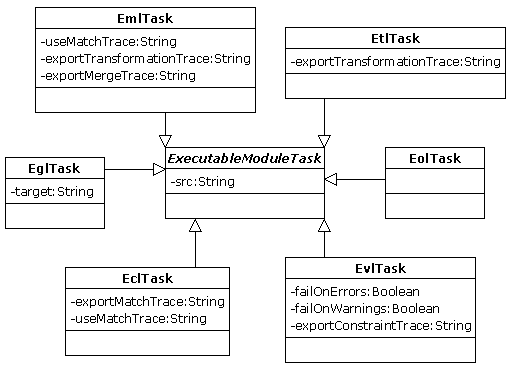
\includegraphics{images/Tasks.png}
	\caption{Model Management Tasks}
	\label{fig:Tasks}
\end{figure}

\subsection{Generic Model Management Task}
\label{sec:EolTask}

The \emph{epsilon.eol} task executes an EOL module, defined using the \emph{src} attribute on the models that are specified using the \emph{model} nested elements.
\subsection{Model Validation Task}
\label{sec:EvlTask}

The \emph{epsilon.evl} task executes an EVL module, defined using the \emph{src} attribute on the models that are specified using the \emph{model} nested elements. In addition to the attributes defined by the ExecutableModuleTask, this task also provides the following attributes:

\begin{itemize}
	\item \emph{failOnErrors} : Errors are the results of unsatisfied constraints. Setting the value of this attribute to \emph{true} (default is \emph{false}) causes a \emph{BuildException} to be raised if one or more errors are identified during the validation process.
	\item \emph{failOnWarnings} : Similarly to errors, warnings are the results of unsatisfied critiques. Setting the value of this atrribute to \emph{true} (default is also \emph{false}) causes a \emph{BuildException} to be raised if one or more warnings are identified during the validation process.
	\item \emph{exportConstraintTrace} : This attribute enables developers to export the internal constraint trace constructed during model validation to the project context so that it can be later accessed by other tasks - which could for example attempt to automatically repair the identified inconsistencies. 
\end{itemize}

\subsection{Model-to-Model Transformation Task}

The \emph{epsilon.etl} task executes an ETL module, defined using the \emph{src} attribute to transform between the models that are specified using the \emph{model} nested elements. In addition to the attributes defined by the ExecutableModuleTask, this task also provides the \emph{exportTransformationTrace} attribute that enables the developer to export the internal transformation trace to the project context. In this way this trace can be reused by subsequent tasks; for example another task can serialize it in the form of a separate traceability model.

\subsection{Model Comparison Task}

The \emph{epsilon.ecl} task executes an ECL module, defined using the \emph{src} attribute to establish matches between elements of the models that are specified using the \emph{model} nested elements. In addition to the attributes defined by the ExecutableModuleTask, this task also provides the \emph{exportMatchTrace} attribute that enables users to export the match-trace calculated during the comparison to the project context so that subsequent tasks can reuse it. For example, as discussed in the sequel, an EML model merging task can use it as a means of identifying correspondences on which to perform merging. In another example, the match-trace can be stored by a subsequent EOL task in the form of an stand-alone weaving model.


\subsection{Model Merging Task}

The \emph{epsilon.eml} task executes an EML module, defined using the \emph{src} attribute on the models that are specified using the \emph{model} nested elements. In addition to the attributes defined by the ExecutableModuleTask, this task also provides the following attributes:

\begin{itemize}
	\item \emph{useMatchTrace} : As discussed in \ref{sec:EML}, to merge a set of models, an EML module needs an established match-trace between elements of the models. The \emph{useMatchTrace} attribute enables the EML task to use a match-trace exported by a preceeding ECL task (using its \emph{exportMatchTrace} attribute).
	\item \emph{exportMergeTrace, exportTransformationTrace} : Similarly to ETL, through these attributes an EML task can export the internal traces calculated during merging for subsequent tasks to use.
\end{itemize}

\subsection{Model-to-Text Transformation Task}
\label{sec:EglTask}
To support model to text transformations, \textit{EglTask (epsilon.egl)} task is provided that executes an Epsilon Generation Language (EGL) module\footnote{As discussed in Section \ref{sec:EGL} EGL has been built atop Epsilon with a minimal contribution of the author}. In addition to the attributes defined by \textit{ExecutableModuleTask}, \textit{EglTask} also defines a \textit{target} attribute that defines where the path of the file where the generated text will be stored.
%!TEX root = ./EpsilonBook.tex

\chapter{Epsilon Flock for Model Migration}
\label{sec:Flock}

The aim of Epsilon Flock is to contribute \emph{model migration} capabilities to Epsilon. Model migration is the process of updating models in response to metamodel changes. This section discusses the motivation for implementing Flock, introduces its syntax and execution semantics, and demonstrates the use of Flock with an example.
Flock can be used to update models to a new version of their metamodel, or even to move from one modelling technology to another (e.g., from XML to EMF).

\section{Background and Motivation}
\label{sec:flock_background}
Model migration involves updating a model in response to changes to the metamodel. Typically, metamodel evolution is accomplished incrementally: changes are made to part of the metamodel and hence model migration typically involves updating only a small proportion of a model's elements \cite{sprinkle03thesis,herrmannsdoerfer08automatability}. Effectively then, model migration is a model-to-model transformation in which the source and target metamodels are similar but not the same. However, as discussed below, model-to-model transformation languages are often cumbersome for specifying model migration.

To illustrate the challenges of model migration, we use the example of metamodel evolution in Figure~\ref{fig:po_mms}. In Figure~\ref{fig:original_po_mm}, a \texttt{Co\-mp\-on\-e\-nt} comprises other \texttt{Co\-mp\-on\-e\-nt}s, \texttt{Co\-nn\-ec\-t\-or}s and \texttt{Po\-rt}s. A \texttt{Co\-nn\-ec\-t\-or} joins two \texttt{Po\-rt}s. \texttt{Co\-nn\-ec\-t\-or}s are unidirectional, and hence define \texttt{to} and \texttt{fr\-om} references to \texttt{Po\-rt}. The original metamodel allows a \texttt{Co\-nn\-ec\-t\-or} to start and end at the same \texttt{Po\-rt}, and the metamodel was evolved to prevent this, as shown in Figure~\ref{fig:evolved_po_mm}. \texttt{Po\-rt} was made abstract, and split into two subtypes, \texttt{In\-p\-utPo\-rt} and \texttt{Ou\-t\-putPo\-rt}. The references between \texttt{Co\-nn\-ec\-t\-or} and (the subtypes of) \texttt{Po\-rt} were renamed for consistency with the names of the subtypes.

%\begin{landscape}
\begin{figure}[htbp]
    \centering
    \subbottom[Original metamodel.]
    {
        \label{fig:original_po_mm}
        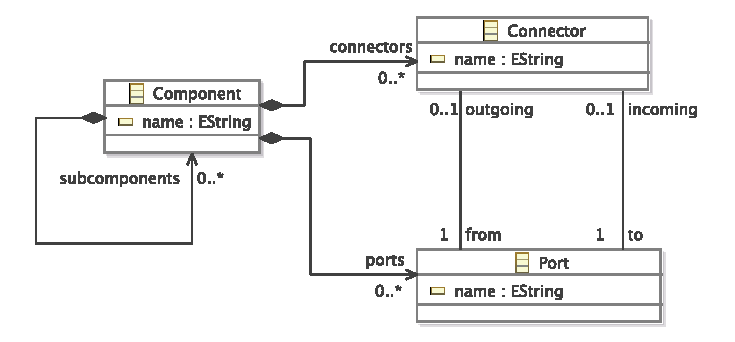
\includegraphics{images/FlockPOExampleOriginal.pdf}
    }
    \subbottom[Evolved metamodel.]
    {
        \label{fig:evolved_po_mm}
        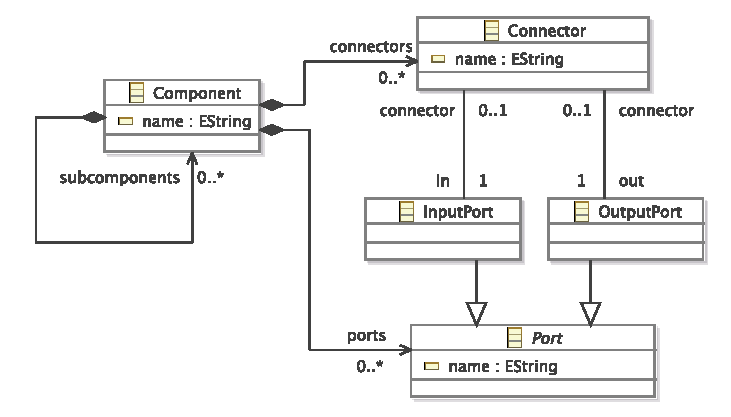
\includegraphics{images/FlockPOExampleEvolved.pdf}
    }
    \caption{Process-oriented metamodel evolution.}
    \label{fig:po_mms}
\end{figure}
%\end{landscape}

Some models that conform to the original metamodel do not conform to the evolved metamodel. Specifically, models might not conform to the evolved metamodel because:

\begin{enumerate}
	\item They contain instances of \texttt{Port}, which is an abstract class in the evolved metamodel.
	\item They contain instances of \texttt{Connector} that specify values for the features \texttt{to} and \texttt{from}, which are not defined for the \texttt{Connector} type in the evolved metamodel.
	\item They contain instances of \texttt{Connector} that do not specify a value for the \texttt{in} and \texttt{out} features, which are mandatory for the \texttt{Connector} type in the evolved metamodel.
\end{enumerate}

Model migration can be achieved with a general-purpose model-to-model transformation using a language such as ETL (Chapter~\ref{sec:ETL}). However, this typically involves writing a large amount of repetitive and redundant code \cite{rose12flock}. Flock reduces the amount of repetitive and redundant code needed to specify model migration by automatically copying from the original to the migrated model all of the model elements that conform to the evolved metamodel as described below.




%\begin{landscape}
\begin{sidewaysfigure}
	\centering
		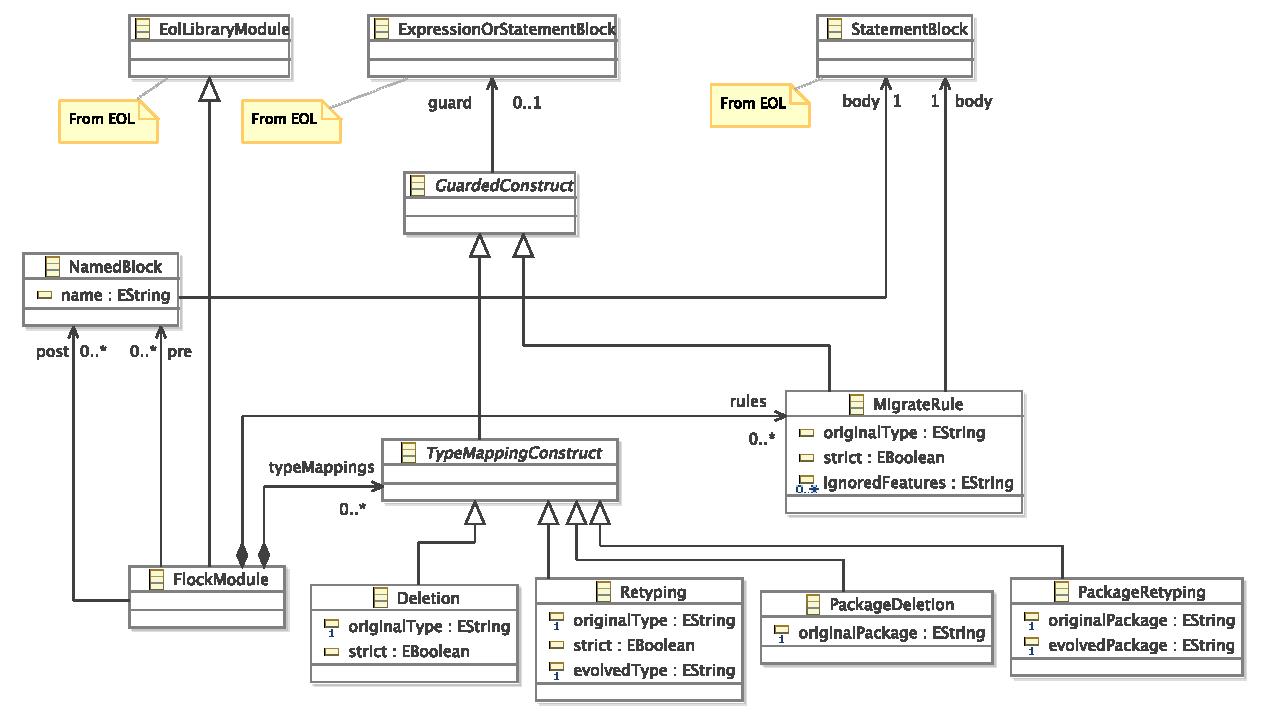
\includegraphics{images/FlockAbstractSyntax.pdf}
	\caption{The Abstract Syntax of Flock}
	\label{fig:flock_abstract_syntax}
\end{sidewaysfigure}
%\end{landscape}


\section{Abstract Syntax}

As illustrated by Figure~\ref{fig:flock_abstract_syntax}, Flock migration strategies are organised into individual modules (\texttt{Flo\-ckMo\-du\-le}). Flock modules inherit from EOL language constructs for specifying user-defined operations and for importing other (EOL and Flock) modules. Like the other rule-based of Epsilon, Flock modules may comprise any number of pre (post) blocks, which are executed before (after) all other constructs. Flock modules comprise any number of type mappings (\texttt{Ty\-peMa\-pp\-i\-ng}) and rules (\texttt{Ru\-le}). Type mappings operate on metamodel types (\texttt{Rety\-pi\-ng} and \texttt{De\-le\-ti\-on}) or on metamodel packages (\texttt{Pa\-ck\-a\-geRety\-pi\-ng} and \texttt{Pa\-ck\-a\-geDe\-le\-ti\-on}). Type mappings are applied to a type in the original metamodel (\texttt{or\-ig\-in\-alTy\-pe}) or to a package in the original metamodel (\texttt{or\-ig\-in\-alPa\-ck\-a\-ge}) . Additionally, \texttt{Rety\-pi\-ng}s apply to an evolved metamodel type (\texttt{ev\-ol\-vedTy\-pe}) or package (\texttt{ev\-ol\-vedPa\-ck\-a\-ge}). Each rule has an original metamodel type (\texttt{or\-ig\-in\-alTy\-pe}), a \texttt{bo\-dy} comprising a block of EOL statements, and zero or more \texttt{ig\-no\-r\-edFe\-at\-ur\-es}. Type mappings and rules can optionally specify a \texttt{gu\-ard}, which is either an EOL statement or a block of EOL statements. Type mappings that operate on metamodel types and rules can be marked as \texttt{str\-ict}.

\section{Concrete Syntax}

Listing \ref{lst:FlockConcreteSyntax} demonstrates the concrete syntax of the Flock language constructs. All of the constructs begin with keyword(s) (\texttt{retype}, \texttt{retype package} \texttt{delete}, \texttt{delete package} or \texttt{migrate}), followed by the original metamodel type or package. Additionally, type mappings that operate on metamodel types and rules can be annotated with the \texttt{strict} modifier. The \texttt{delete} construct can be annotated with a \texttt{cascade} modifier. All constructs can have guards, which are specified using the \texttt{when} keyword.

Migrate rules can specify a list of features that conservative copy will ignore (\texttt{ignoring}), and a \texttt{body} containing a sequence of at least one EOL statement. Note that a migrate rule must have a list of ignored features, or a body, or both.

\begin{lstlisting}[caption={Concrete syntax of Flock retypings, deletions and migrate rules}, label=lst:FlockConcreteSyntax, language=Flock, escapechar=!]
(@strict)?
retype !\textit{<originalType>}! to !\textit{<evolvedType>}!
(when (!\textbf{:}\textit{<eolExpression>}!)|(!\textbf{\{}\textit{<eolStatement>+}\textbf{\}}!))?

retype package !\textit{<originalPackage>}! to !\textit{<evolvedPackage>}!
(when (!\textbf{:}\textit{<eolExpression>}!)|(!\textbf{\{}\textit{<eolStatement>+}\textbf{\}}!))?

(@strict)?
(@cascade)?
delete !\textit{<originalType>}!
(when (!\textbf{:}\textit{<eolExpression>}!)|(!\textbf{\{}\textit{<eolStatement>+}\textbf{\}}!))?

delete package !\textit{<originalPackage>}!
(when (!\textbf{:}\textit{<eolExpression>}!)|(!\textbf{\{}\textit{<eolStatement>+}\textbf{\}}!))?

(@strict)?
migrate !\textit{<originalType>}!
(ignoring !\textit{<featureList>}!)?
(when (!\textbf{:}\textit{<eolExpression>}!)|(!\textbf{\{}\textit{<eolStatement>+}\textbf{\}}!))? {
	!\textit{<eolStatement>}!+
}
\end{lstlisting}

\emph{Pre} and \emph{post} blocks have a simple syntax that, as presented in Listing \ref{lst:FlockPrePostConcreteSyntax}, consists of the identifier (\emph{pre} or \emph{post}), an optional name and the set of statements to be executed enclosed in curly braces.

\begin{lstlisting}[caption=Concrete Syntax of Pre and Post blocks, label=lst:FlockPrePostConcreteSyntax, language=Flock]
(pre|post) <name> {
	statement+
}
\end{lstlisting}

\section{Execution Semantics}
The execution semantics of a Flock module are now described. Note that the Epsilon Model Connectivity (EMC) layer (Chapter~\ref{sec:Design.EMC}), which Flock uses to access and manipulate models supports a range of modelling technologies, and identifies types by name. Consequently, the term \emph{type} is used to mean ``the name of an element of a metamodel'' in the following discussion. For example, \texttt{Co\-mp\-on\-e\-nt}, \texttt{Co\-nn\-ec\-t\-or} and \texttt{In\-p\-utPo\-rt} are three of the types defined in Figure~\ref{fig:evolved_po_mm}.

Execution of a Flock module occurs in six phases:
\begin{enumerate}
  \item Any pre blocks are executed.
  \item Type mapping constructs (retypings and deletions) are processed to identify the way in which original and evolved metamodel types are to be related.
  \item Migrate rules are inspected to build sets of ignored properties.
  \item The information determined in steps 2 and 3 is used as input a copying algorithm, which creates an (equivalent) element in the migrated model for each element of the original model, and copies values from original to equivalent model elements.
  \item Migrate rules are executed on each pair of original and (equivalent) migrated model elements.
  \item Any post blocks are executed.
\end{enumerate}

In phases 2-5, language constructs are executed only when they are \emph{applicable}. The \emph{applicability} of the Flock language constructs (retyping, deletion or migrate rule) is determined from their type and guard. For a language construct $c$ to be applicable to an original model element $o$, $o$ must instantiate either the original type of $c$ or one of the subtypes of the original type of $c$; and $o$ must satisfy the guard of $c$. For language constructs that have been annotated as strict, type-checking is more restrictive: $o$ must instantiate the original type of $c$ (and not one its subtypes). In other words, the applicability of strict constructs is determined with EOL's \texttt{isTypeOf} operation and the applicability of non-strict constructs is determined with EOL's \texttt{isKindOf} operation (Table~\ref{tab:AnyOperations}). For language constructs that have been annotated with cascade, type-checking is less restrictive: $o$ must be contained in another model element (either directly or indirectly) to which the construct is applicable. Similarly, for language constructs that operate on packages (i.e. package retyping and package deletions), type-checking is less restrictive: $o$ must be contained in a package with the same name as the original package of $c$.

Phases 2-4 of execution implement a copying algorithm which has been termed conservative copy and is discussed thoroughly elsewhere \cite{rose12flock}. Essentially, conservative copy will do the following for each element of the original model, $o$:

\begin{enumerate}
	\item \textbf{Do nothing} when $o$ instantiates a type that cannot be instantiated in the evolved metamodel (e.g., because the type of $o$ is now abstract or no longer exists). Example: instances of \texttt{Port} in Figure~\ref{fig:po_mms} are not copied because \texttt{Port} has become abstract.
	\item \textbf{Fully copy} $o$ to produce $m$ in the migrated model when $o$ instantiate a type that has not been at all affected by metamodel evolution. Example: instances of \texttt{Component} in Figure~\ref{fig:po_mms} are fully copied because neither \texttt{Component} nor any of its features have been changed.
	\item \textbf{Partially copy} $o$ to produce $m$ in the migrated model when $o$ instantiates a type with one or more features that have been affected by metamodel evolution. Example: instances of \texttt{Connector} in Figure~\ref{fig:po_mms} are partially copied because the \texttt{from} and \texttt{to} features have been renamed. Note that in a partial copy only the features that have not been affected by metamodel evolution are copied (e.g., the \texttt{name}s of \texttt{Connector}s).
\end{enumerate}

In phase 5, migrate rules are applied. These rules specify the problem-specific migration logic and might, for example, create migrated model elements for original model elements that were skipped or partially copied by the copying algorithm described above. The Flock engine makes available two variables (\texttt{or\-ig\-in\-al} and \texttt{mi\-gr\-at\-ed}) for use in the body of any migration rule. These variables are used to refer to the particular elements of the original and migrated models to which the rule is currently being applied. In addition, Flock defines an \texttt{equivalent()} operation that can be called on any original model element and returns the equivalent migrated model element (or \texttt{null}). The \texttt{equivalent()} operation is used to access elements of the migrated model that cannot be accessed via the \texttt{migrated} variable due to metamodel evolution. Flock rules often contain statements of the form: \texttt{original.x.equivalent()} where \texttt{x} is a feature that has been removed from the evolved metamodel.

Finally, we should consider the order in which Flock schedules language constructs: a construct that appears earlier (higher) in the source file has priority. This is important because only one type mapping (retypings and deletions) is applied per original model element, and because this implies that migrate rules are applied from top-to-bottom. This ordering is consistent with the other languages of the Epsilon platform.


\section{Example}
Flock is now demonstrated using the example of model migration introduced in Section~\ref{sec:flock_background}. Recall that the metamodel evolution in Figure~\ref{fig:po_mms} involves splitting the \texttt{Po\-rt} type to form the \texttt{In\-p\-utPo\-rt} and \texttt{Ou\-tp\-utPo\-rt} types. Figure~\ref{fig:po_migration_strategy} provides a high-level design for migrating models from the original to the evolved metamodel in Figure~\ref{fig:po_mms}.

\begin{figure}[h]
    \begin{framed}
        \footnotesize
        \begin{itemize}
            \item For every instance, p, of \texttt{Port} in the original model: 
            \subitem $-$ If there exists in the original model a \texttt{Connector}, c, that specifies p as the value for its \texttt{from} feature:
            \subsubitem $-$ Create a new instance, i, of \texttt{InputPort} in the migrated model.
            \subsubitem $-$ Set c as the \texttt{connector} of i.
            \subsubitem $-$ Add c to the \texttt{ports} reference of the \texttt{Component} that contains c.
            
            \subitem $-$ If there exists in the original model a \texttt{Connector}, c, that specifies p as the value for its \texttt{to} feature:
            \subsubitem $-$ Create a new instance of \texttt{OutputPort} in the migrated model.
            \subsubitem $-$ Set c as the \texttt{connector} of i.
            \subsubitem $-$ Add c to the \texttt{ports} reference of the \texttt{Component} that contains c.
            
            \item And nothing else changes.
        \end{itemize}
    \end{framed}
    \caption{Model migration strategy in pseudo code for the metamodel evolution in Figure~\ref{fig:po_mms}.}
    \label{fig:po_migration_strategy}
\end{figure}

The Flock migration strategy that implements this design is shown\footnote{Note that \texttt{in} and \texttt{to} are reserved words in EOL, and hence backticks are used to refer to the metamodel features \texttt{in} and \texttt{to} on lines 7, 8 and 16 of Listing~\ref{lst:flock}.} in Listing~\ref{lst:flock}. Three type mappings constructs (on lines 1-4) are used to control the way in which instances of \texttt{Po\-rt} are migrated. For example, line 3 specifies that instances of \texttt{Po\-rt} that are referenced via the \texttt{fr\-om} feature of a \texttt{Co\-nn\-ec\-t\-or} are retyped, becoming \texttt{In\-pu\-tPo\-rt}s. Instances of \texttt{Co\-nn\-ec\-t\-or} are migrated using the rule on lines 6-9, which specifies the way in which the \texttt{fr\-om} and \texttt{to} features have evolved to form the \texttt{in} and \texttt{out} features.

\begin{lstlisting}[float=t,caption=Flock migration strategy for the process-oriented metamodel evolution in Figure~\ref{fig:po_mms}, label=lst:flock, language=Flock]
delete Port when: not (original.isInput() xor original.isOutput())

retype Port to InputPort  when: original.isInput()
retype Port to OutputPort when: original.isOutput()

migrate Connector {
migrated.`in` = original.from.equivalent();
migrated.out = original.`to`.equivalent();
}

operation Original!Port isInput() : Boolean {
return Original!Connector.all.exists(c|c.from == self);
}

operation Original!Port isOutput() : Boolean {
return Original!Connector.all.exists(c|c.`to` == self);
}
\end{lstlisting}


Note that metamodel elements that have not been affected by the metamodel evolution, such as \texttt{Co\-mp\-on\-e\-nt}s, are migrated automatically. Explicit copying code would be needed to achieve this with a general purpose model-to-model transformation language.

\section{Limitations and Scope}
Although Flock has been shown to much more concise than general purpose model-to-model transformation languages for specifying model migration, Flock does not provide some of the features commonly available in general-purpose model-to-model transformation language. This section discusses the limitations of Flock and its intended scope with respect to other tools for model migration.

\subsection{Limitations}
Firstly, Flock does not support rule inheritance, and re-use of migration logic is instead achieved by exploiting the inheritance hierarchy of the original metamodel. The form of re-use provided by Flock is less general than rule-inheritance, but has proved sufficient for existing use-cases.

Secondly, Flock does not provide language constructs for controlling the order in which rules are scheduled (other than the ordering of the rules in the program file). ATL, for example, includes constructs that allow users to specify that rules are scheduled explicitly (lazy rules) or in a memoised manner (unique rules). We anticipate that scheduling constructs might be necessary for larger migration strategies, but have not yet encountered situations in which they have been required.

Thirdly, Flock is tailored for applying migration to a single original and a single migrated model. Although further models can be accessed by a Flock migration strategy, they cannot be used as the source or target of the conservative copy algorithm. By contrast, some general-purpose model transformation languages can access and manipulate any number of models.

Finally, Flock has been tailored to the model migration problem. In other words, we believe that Flock is well-suited to specifying model transformations between two metamodels that are very similar. For metamodel evolution in which the original metamodel undergoes significant and large-scale revision, a general-purpose transformation might be more suitable than Flock for specifying model migration.

\subsection{Scope}
Flock is typically used as a manual specification approach in which model migration strategies are written by hand. As such, we believe that Flock provides a flexible and concise way to specify migration, and is a foundation for further tools that seek to automate the metamodel evolution and model migration processes. There are approaches to model migration that encompass both the metamodel evolution and model migration processes, seeking to automatically derive model migration strategies (e.g., Edapt \url{http://www.eclipse.org/edapt/}). These approaches provide more automation but at the cost of flexibility: for example, you might be restricted to using a tool-specific editor to perform model migration, or to using only EMF.


\section{Further Reading}
Further examples of applying Flock include migration of UML activity diagrams (at Transformation Tool Contest 2010 workshop\footnote{\url{http://planet-mde.org/ttc2010/}}), and migration of UML class diagrams, GMF models, and a domain-specific modelling language for NNTP newsgroups in Rose's doctoral thesis \cite{rose11thesis}.

A more thorough discussion of the design decisions and execution semantics of Flock can be found in a SoSyM journal article \cite{rose12flock}. Flock has been compared with other model migration tools and languages in a MoDELS paper \cite{rose10comparison}. 

\subsection{Pattern Matching Task}

The \emph{epsilon.epl} task executes an EPL module, defined using the \emph{src} attribute to perform pattern matching on the models that are specified using the \emph{model} nested elements. In addition to the attributes defined by the ExecutableModuleTask, this task also provides the following attributes.

\begin{itemize}
  \item \emph{repeatWhileMatches}: A boolean specifying whether the pattern matching process should continue to execute for as long as matches are found.
  \item \emph{maxLoops}: An integer specifying the maximum number of pattern matching iterations.
  \item \emph{exportAs}: The name under which the computed pattern match model should be made available to other Epsilon tasks of the workflow.
\end{itemize}


\subsection{Adding a new Model Management Task}
\label{sec:Workflow.NewModelManagementTask}

As discussed in Section \ref{sec:Design.ImplementingANewLanguage}, additional task-specific languages are likely to be needed in the future for tasks that are not effectively supported by existing task-specific languages. In addition to designing and implementing the syntax and execution semantics of a new language, it is also important to provide integration with the workflow -- if the nature of the language permits execution within a workflow. As a counter-example, no workflow task has been provided for EWL since its execution semantics is predominately user-driven and as such, it makes little sense to execute EWL in the context of an automated workflow.

To implement support for a new task-specific language to the workflow, a new extension of the abstract \emph{ExecutableModuleTask} needs to be provided (similarly to what has been done for existing task-specific languages). By extending \emph{ExecutableModuleTask}, the task is automatically provided with access to the essential features of the workflow such as the shared model repository, and runtime context. Additional configuration options for the task need to specified as new ANT \emph{attributes} and/or \emph{nested elements}, similarly to what has been done for the tasks presented in Sections \ref{sec:EolTask}--\ref{sec:EglTask}.

\section{Chapter Summary}

This chapter has presented the detailed design of an ANT-based framework for integrating and orchestrating mainstream software development tasks with model management tasks implemented using model management languages in Epsilon. In Section \ref{sec:Workflow.Framework}, the core framework that provides features such centralized model loading/storing facilities, a shared model repository and a mechanism through which individual tasks can communicate at runtime has been illustrated. Then, Section \ref{sec:Workflow.ModelManagementTasks} has provided a discussion on the integration of the task specific languages with the framework and also provided guidance for adding support for additional languages that are likely to be developed in the future atop Epsilon.

\clearpage
\chapter{The Epsilon Unit Testing Framework (EUnit)}
\label{chp:eunit}

EUnit is an unit testing framework specifically designed to test model management tasks, based on EOL and the Ant workflow tasks. It provides assertions for comparing models, files and directories. Tests can be reused with different sets of models and input data, and differences between the expected and actual models can be graphically visualized. This chapter discusses the motivation behind EUnit, describes how tests are organized and written and shows two examples of how a model-to-model transformation can be tested with EUnit. This chapter ends with a discussion of how EUnit can be extended to support other modelling and model management technologies.

\section{Motivation}
\label{sec:eunit-motiv-test-model}

Model-driven approaches are being adopted in a wide range of demanding environments, such as finance, health care or telecommunications~\cite{Guttman2006}. In this context, validation and verification is identified as one of the many challenges of model-driven software engineering (MDSE)~\cite{Chaudron2009}.

MDSE in practice involves creating models, and thereafter \textit{managing} them, via various tasks, such as model transformation, validation and merging.  The validation and verification of each type of model management task has its own specific challenges. Kolovos et al.\ list testing concerns for model-to-model (M2M) and model-to-text (M2T) transformations, model validations, model comparisons and model compositions in~\cite{EUnit}. Baudry et al.\ identify three main issues when testing model transformations~\cite{Baudry2010}: the complexity of the input and output models, the immaturity of the model management environments and the large number of different transformation languages and techniques.

\subsection{Common Issues}
\label{sec:eunit-common-issues}

While each type of model management task does have specific complexity, some of the concerns raised by Baudry can be generalized to apply to all model management tasks:
\begin{itemize}
\item There is usually a large number of models to be handled. Some may be created by hand, some may be generated using hand-written programs, and some may be generated automatically following certain coverage criteria.

\item A single model or set of models may be used in several tasks. For instance, a model may be validated before performing an in-place transformation to assist the user, and later on it may be transformed to another model or merged with a different model. This requires having at least one test for each valid combination of models and sets of tasks.

\item Test oracles are more complex than in traditional unit testing~\cite{Mottu2008}: instead of checking scalar values or simple lists, entire graphs of model objects or file trees may have to be compared. In some cases, complex properties in the generated artifacts may have to be checked.

\item Models and model management tasks may use a wide range of technologies. Models may be based on Ecore~\cite{Steinberg2008}, XML files or Java object graphs, among many others. At the same time, tasks may use technologies from different platforms, such as Epsilon, oAW~\cite{oAW} or AMMA~\cite{AMMA}. Many of these technologies offer high-level tools for running and debugging the different tasks using several models. However, users wishing to do automated unit testing need to learn low-level implementation details about their modelling and model management technologies. This increases the initial cost of testing these tasks and hampers the adoption of new technologies.

\item Existing testing tools tend to focus on the testing technique itself, and lack integration with external systems. Some tools provide graphical user interfaces, but most do not generate reports which can be consumed by a continuous integration server, for instance.
\end{itemize}

\subsection{Testing with JUnit}
\label{sec:testing-with-junit}

The previous issues are easier to understand with a concrete example. This section shows how a simple transformation between two EMF models in ETL using JUnit 4~\cite{JUnit2011} would be normally tested, and points out several issues due to JUnit's limitations as a general-purpose unit testing framework for Java programs.

For the sake of brevity, only an outline of the JUnit test suite is included. All JUnit test suites are defined as Java classes. This test suite has three methods:

\begin{enumerate}
\item The test setup method (marked with the \javaannotation{Before} JUnit annotation) loads the required models by creating and configuring instances of \class{EmfModel}. After that, it prepares the transformation by creating and configuring an instance of \class{EtlModule}, adding the input and output models to its model repository.

\item The test case itself (marked with \javaannotation{Test}) runs the ETL transformation and uses the generic comparison algorithm implemented by EMF Compare to perform the model comparison.

\item The test teardown method (marked with \javaannotation{After}) disposes of the models.
\end{enumerate}

Several issues can be identified in each part of the test suite. First, test setup is tightly bound to the technologies used: it depends on the API of the \class{EmfModel} and \class{EtlModule} classes, which are both part of Epsilon. Later refactorings in these classes may break existing tests.

The test case can only be used for a single combination of input and output models. Testing several combinations requires either repeating the same code and therefore making the suite less maintainable, or using parametric testing, which may be wasteful if not all tests need the same combinations of models.

Model comparison requires the user to manually select a model comparison engine and integrate it with the test. For comparing EMF models, EMF Compare is easy to use and readily available. However, generic model comparison engines may not be available for some modelling technologies, or may be harder to integrate.

Finally, instead of comparing the obtained and expected models, several properties could have been checked in the obtained model. However, querying models through Java code can be quite verbose.

\subsection{Selected Approach}
\label{sec:eunit-selected-approach}

Several approaches could be followed to address these issues. Our first instinct would be to extend JUnit and reuse all the tooling available for it. A custom test runner would simplify setup and teardown, and modelling platforms would integrate their technologies into it. Since Java is very verbose when querying models, the custom runner should run tests in a higher-level language, such as EOL. However, JUnit is very tightly coupled to Java, and this would impose limits on the level of integration we could obtain. For instance, errors in the model management tasks or the EOL tests could not be reported from their original source, but rather from the Java code which invoked them.  Another problem with this approach is that new integration code would need to be written for each of the existing platforms.

Alternatively, we could add a new language exclusively dedicated to testing to the Epsilon family.  Being based on EOL, model querying would be very concise, and with a test runner written from scratch, test execution would be very flexible. However, this would still require all platforms to write new code to integrate with it, and this code would be tightly coupled to Epsilon.

As a middle ground, we could decorate EOL to guide its execution through a new test runner, while reusing the Apache Ant~\cite{ANT} tasks already provided by several of the existing platforms, such as AMMA or Epsilon. Like Make, Ant is a tool focused on automating the execution of processes such as program builds. Unlike Make, Ant defines processes using XML \emph{buildfiles} with sets of interrelated \emph{targets}. Each target contains in turn a sequence of \emph{tasks}. Many Ant tasks and Ant-based tools already exist, and it is easy to create a new Ant task.

Among these three approaches, EUnit follows the last one. Ant tasks take care of model setup and management, and tests are written in EOL and executed by a new test runner, written from the ground up.

\section{Test Organization}
\label{sec:eunit-test-organization}

EUnit has a rich data model: test suites are organized as trees of tests, and each test is divided into many parts which can be extended by the user. This section is dedicated to describing how test suites and tests are organized. The next section indicates how they are written.

\subsection{Test Suites}

EUnit test suites are organized as trees: inner nodes group related test cases and define \emph{data} bindings. Leaf nodes define \emph{model} bindings and run the test cases.

Data bindings repeat all test cases with different values in one or more variables. They can implement parametric testing, as in JUnit 4. EUnit can nest several data bindings, running all test cases once for each combination.

Model bindings are specific to EUnit: they allow developers to repeat a single test case with different subsets of models. Data and model bindings can be combined. One interesting approach is to set the names of the models to be used in the model binding from the data binding, as a quick way to try several test cases with the same subsets of models.

\begin{figure}
  \centering
  % -*- mode: latex -*-
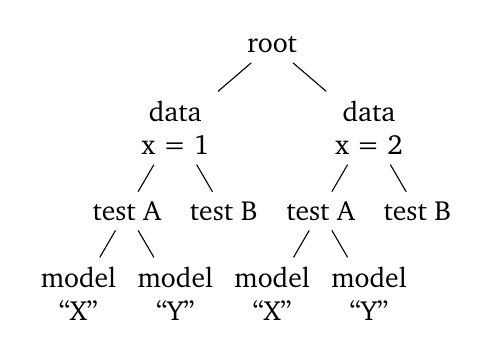
\begin{tikzpicture}
  \newcommand{\databox}[1]{\parbox{2.5em}{\centering data #1}}
  \newcommand{\withbox}[1]{\parbox{3em}{\centering model #1}}

  \node (root) {root}[
  level 1/.style={sibling distance=7em},
  level 2/.style={sibling distance=3.5em},
  level distance=3em,
  ]
  child {
    node (data1) {\databox{x = 1}}
    child {node (t2mb1) {test A}
      child {node (t2mb1a) {\withbox{\modelname{X}}}}
      child {node (t2mb1b) {\withbox{\modelname{Y}}}}
    }
    child {node (t1mb1) {test B}}
  }
  child  {
    node (data2) {\databox{x = 2}}
    child {node (t2mb2) {test A}
      child {node (t2mb2a) {\withbox{\modelname{X}}}}
      child {node (t2mb2b) {\withbox{\modelname{Y}}}}
    }
    child {node (t1mb2) {test B}}
  };
\end{tikzpicture}

  \caption{Example of an EUnit test tree}
  \label{fig:eunit-test-tree}
\end{figure}

Figure~\ref{fig:eunit-test-tree} shows an example of an EUnit test tree: nodes with data bindings are marked with \eol{data}, and nodes with model bindings are marked with \eol{model}. EUnit will perform a preorder traversal of this tree, running the following tests:
\begin{enumerate}
\item \test{A} with \variable{x = 1} and model X.
\item \test{A} with \variable{x = 1} and model Y.
\item \test{B} with \variable{x = 1} and both models.
\item \test{A} with \variable{x = 2} and model X.
\item \test{A} with \variable{x = 2} and model Y.
\item \test{B} with \variable{x = 2} and both models.
\end{enumerate}

Optionally, EUnit can filter tests by name, running only \test{A} or \test{B}. Similarly to JUnit, EUnit logs start and finish times for each node in the tree, so the most expensive test cases can be quickly detected. However, EUnit logs CPU time\footnote{CPU time only measures the time elapsed in the thread used by EUnit, and is more stable with varying system load in single-threaded programs.} in addition to the usual wallclock time.

Parametric testing is not to be confused with \emph{theories}~\cite{Saff2007}: both repeat a test case with different values, but results are reported quite differently. While parametric testing produces separate test cases with independent results, theories produce aggregated tests which only pass if the original test case passes for every data point. Figure~\ref{fig:parametric-vs-theories} illustrates these differences. EUnit does not support theories yet: however, they can be approximated with data bindings.

\begin{figure}
  \centering
  \subbottom[Parametric testing]{
    % -*- latex -*-
\providecommand{\typea}{data}
\providecommand{\typeb}{test}

\begin{tikzpicture}
  \newcommand{\tsub}[1]{\textsubscript{#1}}
  \node {root}[
  level 1/.style={sibling distance=7em},
  level 2/.style={sibling distance=3.5em},
  level distance=3em,
  ]
  child {
    node {\typea\tsub{1}}
    child {
      node {\typeb\tsub{1}}
    }
    child {
      node {\typeb\tsub{2}}
    }
  }
  child {
    node {\typea\tsub{2}}
    child {
      node {\typeb\tsub{1}}
    }
    child {
      node {\typeb\tsub{2}}
    }
  };
\end{tikzpicture}

  }
  \subbottom[Theories]{
    \newcommand{\typea}{test}
    \newcommand{\typeb}{data}
    % -*- latex -*-
\providecommand{\typea}{data}
\providecommand{\typeb}{test}

\begin{tikzpicture}
  \newcommand{\tsub}[1]{\textsubscript{#1}}
  \node {root}[
  level 1/.style={sibling distance=7em},
  level 2/.style={sibling distance=3.5em},
  level distance=3em,
  ]
  child {
    node {\typea\tsub{1}}
    child {
      node {\typeb\tsub{1}}
    }
    child {
      node {\typeb\tsub{2}}
    }
  }
  child {
    node {\typea\tsub{2}}
    child {
      node {\typeb\tsub{1}}
    }
    child {
      node {\typeb\tsub{2}}
    }
  };
\end{tikzpicture}

  }
  \caption{Comparison between parametric testing and theories}
  \label{fig:parametric-vs-theories}
\end{figure}

\subsection{Test Cases}
\label{sec:eunit-test-cases}

The execution of a test case is divided into the following steps:
\begin{enumerate}
\item Apply the data bindings of its ancestors.
\item Run the model setup sections defined by the user.
\item Apply the model bindings of this node.
\item Run the regular setup sections defined by the user.
\item Run the test case itself.
\item Run the teardown sections defined by the user.
\item Tear down the data bindings and models for this test.
\end{enumerate}

An important difference between JUnit and EUnit is that setup is split into two parts: model setup and regular setup. This split allows users to add code before and after model bindings are applied. Normally, the model setup sections will load all the models needed by the test suite, and the regular setup sections will further prepare the models selected by the model binding. Explicit teardown sections are usually not needed, as models are disposed automatically by EUnit. EUnit includes them for consistency with the xUnit frameworks.

Due to its focus on model management, model setup in EUnit is very flexible. Developers can combine several ways to set up models, such as model references, individual Apache Ant~\cite{ANT} tasks, Apache Ant targets or Human-Usable Text Notation (HUTN)~\cite{HUTN} fragments.

A test case may produce one among several results. \eol{SUCCESS} is obtained if all assertions passed and no exceptions were thrown. \eol{FAILURE} is obtained if an assertion failed. \eol{ERROR} is obtained if an unexpected exception was thrown while running the test. Finally, tests may be \eol{SKIPPED} by the user.

\section{Test Specification}
\label{sec:eunit-test-specification}

In the previous section, we described how test suites and test cases are organized. In this section, we will show how to write them.

As discussed before, after evaluating several approaches, we decided to combine the expressive power of EOL and the extensibility of Apache Ant. For this reason, EUnit test suites are split into two files: an Ant buildfile and an EOL script with some special-purpose annotations. The next subsections describe the contents of these two files and revisit the previous example with EUnit.

\subsection{Ant Buildfile}

EUnit uses standard Ant buildfiles: running EUnit is as simple as using its Ant task. Users may run EUnit more than once in a single Ant launch: the graphical user interface will automatically aggregate the results of all test suites.

\subsubsection{EUnit Invocations}

An example invocation of the EUnit Ant task using the most common features is shown in Listing~\ref{lst:example-eunit-ant}. Users will normally only use some of these features at a time, though. Optional attributes have been listed between brackets. Some nested elements can be repeated 0+ times (\verb!*!) or 0-1 times (\verb!?!). Valid alternatives for an attribute are separated with \verb!|!.

\begin{lstlisting}[language=XML,columns=fixed,caption=Format of an invocation of the EUnit Ant task,label=lst:example-eunit-ant]
<epsilon.eunit src="..."
    [failOnErrors="..."]
    [package=".."]
    [toDir="..."]
    [report="yes|no"]>
  (<model     ref="OldName" [as="NewName"]/>)*
  (<uses      ref="x" [as="y"] />)*
  (<exports   ref="z" [as="w"] />)*
  (<parameter name="myparam" value="myvalue" />)*
  (<modelTasks><!-- Zero or more Ant tasks --></modelTasks>)?
</epsilon.eunit>
\end{lstlisting}

The EUnit Ant task is based on the Epsilon abstract executable module task (see Section~\ref{sec:ExecutableModuleTask}), inheriting some useful features. The attribute \xmlattribute{src} points to the path of the EOL file, and the optional attribute \xmlattribute{failOnErrors} can be set to \eol{false} to prevent EUnit from aborting the Ant launch if a test case fails. EUnit also inherits support for importing and exporting global variables through the \xmlelement{uses} and \xmlelement{exports} elements: the original name is set in \xmlattribute{ref}, and the optional \xmlattribute{as} attribute allows for using a different name. For receiving parameters as name-value piars, the \xmlelement{parameter} element can be used.

Model references (using the \xmlelement{model} nested element) are also inherited from the Epsilon abstract executable module task. These allow model management tasks to refer by name to models previously loaded in the Ant buildfile. However, EUnit implicitly reloads the models after each test case. This ensures that test cases are isolated from each other.

The EUnit Ant task adds several new features to customize the test result reports and perform more advanced model setup. By default, EUnit generates reports in the XML format of the Ant \xmlelement{junit} task. This format is also used by many other tools, such as the TestNG unit testing framework~\cite{TestNG}, the Jenkins continuous integration server~\cite{Jenkins} or the JUnit Eclipse plug-ins. To suppress these reports, \xmlattribute{report} must be set to \xmlattribute{no}.

By default, the XML report is generated in the same directory as the Ant buildfile, but it can be changed with the \xmlattribute{toDir} attribute. Test names in JUnit are formed by its Java package, class and method: EUnit uses the filename of the EOL script as the class and the name of the EOL operation as the method. By default, the package is set to the string ``default'': users are encouraged to customize it with the \xmlattribute{package} attribute.

The optional \xmlelement{modelTasks} nested element contains a sequence of Ant tasks which will be run after reloading the model references and before running the model setup sections in the EOL file. This allows users to run workflows more advanced than simply reloading model references, such as the one in Listing~\ref{lst:eunit-ex1-ant}.

\subsubsection{Helper Targets}

Ant buildfiles for EUnit may include \emph{helper targets}. These targets can be invoked using \eol{runTarget("targetName")} from anywhere in the EOL script. Helper targets are quite versatile: called from an EOL model setup section, they allow for reusing model loading fragments between different EUnit test suites. They can also be used to invoke the model management tasks under test. Listing~\ref{lst:eunit-ex1-ant} shows a helper target for an ETL transformation, and listing~\ref{lst:eunit-atl} shows a helper target for an ATL transformation.

\subsection{EOL script}
\label{sec:eunit-eol-script}

The Epsilon Object Language script is the second half of the EUnit test suite. EOL annotations are used to tag some of the operations as data binding definitions (\eolannotation{@data} or \eolannotation{@Data}), additional model setup sections (\eolannotation{@model}/\eolannotation{@Model}), test setup and teardown sections (\eolannotation{@setup}/\eolannotation{@Before} and \eolannotation{@teardown}/\eolannotation{@After}) and test cases (\eolannotation{@test}/\eolannotation{@Test}). Suite setup and teardown sections can also be defined with \eolannotation{@suitesetup}/\eolannotation{@BeforeClass} and \eolannotation{@suiteteardown}/\eolannotation{@AfterClass} annotations: these operations will be run before and after all tests, respectively.

\subsubsection{Data bindings}

Data bindings repeat all test cases with different values in some variables. To define a data binding, users must define an operation which returns a sequence of elements and is marked with \eolannotation{@data variable}. All test cases will be repeated once for each element of the returned sequence, setting the specified variable to the corresponding element. Listing~\ref{lst:eunit-databind} shows two nested data bindings and a test case which will be run four times: with \variable{x=1} and \variable{y=5}, \variable{x=1} and \variable{y=6}, \variable{x=2} and \variable{y=5} and finally \variable{x=2} and \variable{y=6}. The example shows how \variable{x} and \variable{y} could be used by the setup section to generate an input model for the test. This can be useful if the intent of the test is ensuring that a certain property holds in a class of models, rather than a single model.

\begin{lstlisting}[language=EOL,caption=Example of a 2-level data binding,label=lst:eunit-databind,columns=fixed]
@data x
operation firstLevel()  { return 1.to(2); }

@data y
operation secondLevel() { return 5.to(6); }

@setup
operation generateModel() { -* generate model using x and y *- }

@test
operation mytest() { -* test with the generated model *- }
\end{lstlisting}

Alternatively, if both \variable{x} and \variable{y} were to use the same sets of values, we could add two \eolannotation{@data} annotations to the same operation. For instance, Listing~\ref{lst:eunit-databind-reused} shows how we could test with 4 cases: \variable{x=1} and \variable{y=1}, \variable{x=1} and \variable{y=2}, \variable{x=2} and \variable{y=1} and \variable{x=2} and \variable{y=2}.

\begin{lstlisting}[language=EOL,caption=Example of reusing the same operation for several data bindings,label=lst:eunit-databind-reused,columns=fixed]
@data x
@data y
operation levels()  { return 1.to(2); }

@setup
operation generateModel() { -* generate model using x and y *- }

@test
operation mytest() { -* test with the generated model *- }
\end{lstlisting}

\subsubsection{Model bindings}

Model bindings repeat a test case with different subsets of models. They can be defined by annotating a test case with \eolannotation{\$with map} or \eolannotation{\$onlyWith map} one or more times, where \eol{map} is an EOL expression that produces a \class{Map}. For each key-value pair \variable{key = value}, EUnit will rename the model named \variable{value} to \variable{key}. The difference between \eolannotation{\$with} and \eolannotation{\$onlyWith} is how they handle the models not mentioned in the \class{Map}: \eolannotation{\$with} will preserve them as is, and \eolannotation{\$onlyWith} will make them unavailable during the test. \eolannotation{\$onlyWith} is useful for tightly restricting the set of available models in a test and for avoiding ambiguous type references when handling multiple models using the same metamodel.

Listing~\ref{lst:eunit-modelbind} shows two tests which will be each run twice. The first test uses \eolannotation{\$with}, which preserves models not mentioned in the \class{Map}: the first time, model \modelname{A} will be the default model and model \modelname{B} will be the \modelname{Other} model, and the second time, model \modelname{B} will be the default model and model \modelname{A} will be the \modelname{Other} model. The second test uses two \eolannotation{\$onlyWith} annotations: on the first run, \modelname{A} will be available as \modelname{Model} and \modelname{B} will not unavailable, and on the second run, only \modelname{B} will be available as \modelname{Model} and \modelname{A} will be unavailable.

\begin{lstlisting}[float=tbp, language=EOL,caption=Examples of model bindings,label=lst:eunit-modelbind,columns=fixed]
$with Map {"" = "A", "Other" = "B"}
$with Map {"" = "B", "Other" = "A"}
@test
operation mytest() {
  -* use the default and Other models, while
     keeping the rest as is *-
}

$onlyWith Map { "Model" = "A" }
$onlyWith Map { "Model" = "B" }
@test
operation mytest2() {
  -- first time: A as 'Model', B is unavailable
  -- second time: B as 'Model', A is unavailable
}
\end{lstlisting}

\subsubsection{Additional variables and built-in operations}

EUnit provides several variables and operations which are useful for testing. These are listed in Table~\ref{tab:eunit-operations}.

\begin{longtabu} {|p{6cm}|X|}
  \caption{Extra operations and variables in EUnit}
  \label{tab:eunit-operations}\\
 
    \hline \textbf{Signature} & \textbf{Description}  \\\hline

    runTarget(name : String)      & Runs the specified target of the Ant buildfile which invoked EUnit. \\\hline

    exportVariable(name : String) & Exports the specified variable, to be used by another executable module (see Section~\ref{sec:ExecutableModuleTask}). \\\hline

    useVariable(name : String) & Imports the specified variable, which should have been previously exported by another executable module (see Section~\ref{sec:ExecutableModuleTask}). \\\hline

    loadHutn(name : String, hutn : String) & Loads an EMF model with the specified name, by parsing the second argument as an HUTN~\cite{HUTN} fragment. \\\hline

    antProject : org.apache.tools.ant.Project & Global variable which refers to the Ant project being executed. This can be used to create and run Ant tasks from inside the EOL code. \\\hline
  \end{longtabu}


\subsubsection{Assertions}

EUnit implements some common assertions for equality and inequality, with special versions for comparing floating-point numbers. EUnit also supports a limited form of exception testing with \eol{assertError}, which checks that the expression inside it throws an exception. Custom assertions can be defined by the user with the \eol{fail} operation, which fails a test with a custom message. The available assertions are shown in Table~\ref{tab:eunit-assertions}. Table~\ref{tab:eunit-comparator-options} lists the available option keys which can be used with the model equality assertions, by comparator.

More importantly, EUnit implements specific assertions for comparing models, files and trees of files. Model comparison is not implemented by the assertions themselves: it is an optional service implemented by some EMC drivers. Currently, EMF models will automatically use EMF Compare as their comparison engine. The rest of the EMC drivers do not support comparison yet.  The main advantage of having an abstraction layer implement model comparison as a service is that the test case definition is decoupled from the concrete model comparison engine used.

Model, file and directory comparisons take a snapshot of their operands before comparing them, so EUnit can show the differences right at the moment when the comparison was performed. This is especially important when some of the models are generated on the fly by the EUnit test suite, or when a test case for code generation may overwrite the results of the previous one.

Figure~\ref{fig:screenshot-eunit} shows a screenshot of the EUnit graphical user interface. On the left, an Eclipse view shows the results of several EUnit test suites. We can see that the \eol{load-\allowbreak{}models-\allowbreak{}with-\allowbreak{}hutn} suite failed. The Compare button to the right of ``Failure Trace'' can be pressed to show the differences between the expected and obtained models, as shown on the right side. EUnit implements a pluggable architecture where \emph{difference viewers} are automatically selected based on the types of the operands. There are difference viewers for EMF models, file trees and a fallback viewer which converts both operands to strings.

\newcommand{\parameter}[1]{\newline{}\phantom{- }#1}
\begin{longtabu}{|p{6.5cm}|X|}
  \caption{Assertions in EUnit}
  \label{tab:eunit-assertions} \\\hline

  \textbf{Signature} & \textbf{Description}  \\\hline

  assertTrue([msg : String,]\parameter{cond : Boolean}) & Fails the test with the optional message \variable{msg} if \variable{cond} is \eol{false}.\\\hline

  assertEquals([msg : String,]\parameter{expected : Any},\parameter{obtained : Any}) & Fails the test with the optional message \variable{msg} if the values of \variable{expected} and \variable{obtained} are not equal. \\\hline

  assertEquals([msg : String,]\parameter{expected : Real},\parameter{obtained : Real},\parameter{ulps : Integer}) & Fails the test with the optional message \variable{msg} if the values of \variable{expected} and \variable{obtained} differ in more than \variable{ulps} units of least precision. See \href{http://download.oracle.com/javase/6/docs/api/java/lang/Math.html\#ulp(double)}{this site} for details.\\\hline

  assertEqualModels(\parameter{[msg : String,]}\parameter{expectedModel : String},\parameter{obtainedModel : String}\parameter{[options : Map]}) & Fails the test with the optional message \variable{msg} if the model named \variable{obtainedModel} is not equal to the model named \variable{expectedModel}. Model comparisons are performed on snapshots of the resource sets of both models. During EMF comparisons, XMI identifiers are ignored. Additional comparator-specific options can be specified through \variable{options}.\\\hline

  assertEqualFiles(\parameter{expectedPath : String},\parameter{obtainedPath : String}) & Fails the test if the contents of the file in \variable{obtainedPath} differ from those of the file in \variable{expectedPath}. File comparisons are performed on snapshots of both files.\\\hline

  assertEqualDirectories(\parameter{expectedPath : String},\parameter{obtainedPath : String}) & Fails the test if the contents of the directory in \variable{obtainedFile} differ from those of the directory in \variable{expectedPath}. Directory comparisons are performed on recursive snapshots of both directories.\\\hline

  assertError(expr : Any) & Fails the test if no exception is thrown during the evaluation of \variable{expr}.\\\hline

  fail(msg : String) & Fails a test with the message \variable{msg}.\\\hline

  assertFalse([msg : String,]\parameter{cond : Boolean}) & Fails the test with the optional message \variable{msg} if \variable{cond} is \eol{true}. It is a negated version of assertTrue. \\\hline

  assertNotEquals([msg : String,]\parameter{expected : Any},\parameter{obtained : Any}) & Negated version of assertEquals([msg : String,] expected : Any, obtained : Any). \\\hline

  assertNotEquals([msg : String,]\parameter{expected : Real},\parameter{obtained : Real},\parameter{ulps : Integer}) & Negated version of assertEquals([msg : String,] expected : Real, obtained : Real, ulps : Integer). \\\hline

  assertNotEqualModels(\parameter{[msg : String,]}\parameter{expectedModel : String},\parameter{obtainedModel : String}) & Negated version of assertNotEqualModels.\\\hline

  assertNotEqualFiles(\parameter{expectedPath : String},\parameter{obtainedPath : String}) & Negated version of assertEqualFiles.\\\hline

  assertNotEqualDirectories(\parameter{expectedPath : String},\parameter{obtainedPath : String}) & Negated version of assertEqualDirectories.\\\hline
\end{longtabu}

\begin{longtabu}{|p{3cm}|p{3cm}|X|}
  \caption{Available options by model comparator}
  \label{tab:eunit-comparator-options} \\\hline

  \textbf{Comparator} & \textbf{Key} & \textbf{Usage}  \\\hline
  EMF & ``whitespace'' & When set to ``ignore'', differences in attribute values due to whitespace will be ignored. \\\hline
\end{longtabu}

\begin{sidewaysfigure}
  \centering
  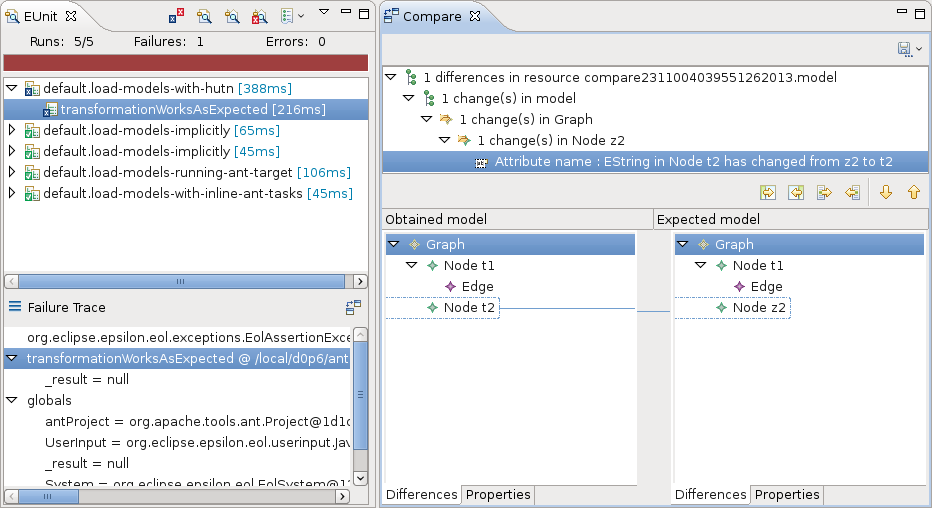
\includegraphics[width=\textwidth]{images/EUnitUI}
  \caption{Screenshot of the EUnit graphical user interface}
  \label{fig:screenshot-eunit}
\end{sidewaysfigure}

\section{Examples}
\label{sec:eunit-examples}

\subsection{Models and Tasks in the Buildfile}
\label{sec:eunit-exampl-balanc-ant}

After describing the basic syntax, we will show how to use EUnit to test an ETL transformation.

The Ant buildfile is shown in Listing~\ref{lst:eunit-ex1-ant}. It has two targets: \anttarget{run-tests} (lines 2--16) invokes the EUnit suite, and \anttarget{tree2graph} (lines 17--22) is a helper target which transforms model \modelname{Tree} into model \modelname{Graph} using ETL. The \xmlelement{modelTasks} nested element is used to load the input, expected output and output EMF models. \modelname{Graph} is loaded with \xmlattribute{read} set to \eol{false}: the model will be initially empty, and will be populated by the ETL transformation.

\begin{lstlisting}[language=XML, caption=Ant buildfile for EUnit with \xmlelement{modelTasks} and a helper target, label=lst:eunit-ex1-ant]
<project>
  <target name="run-tests">
    <epsilon.eunit src="test-external.eunit">
      <modelTasks>
        <epsilon.emf.loadModel name="Tree"
            modelfile="tree.model"
            metamodelfile="tree.ecore"
            read="true" store="false"/>
        <epsilon.emf.loadModel name="GraphExpected"
            modelfile="graph.model"
            metamodelfile="graph.ecore"
            read="true" store="false"/>
        <epsilon.emf.loadModel name="Graph"
            modelfile="transformed.model"
            metamodelfile="graph.ecore"
            read="false" store="false"/>
      </modelTasks>
    </epsilon.eunit>
  </target>
  <target name="tree2graph">
    <epsilon.etl src="${basedir}/resources/Tree2Graph.etl">
      <model ref="Tree"/>
      <model ref="Graph"/>
    </epsilon.etl>
  </target>
</project>
\end{lstlisting}

The EOL script is shown in Listing~\ref{lst:eunit-ex1-eol}: it invokes the helper task (line 3) and checks that the obtained model is equal to the expected model (line 4). Internally, EMC will perform the comparison using EMF Compare.

\begin{lstlisting}[language=EOL, caption=EOL script using \eol{runTarget} to run ETL, label=lst:eunit-ex1-eol]
@test
operation transformationWorksAsExpected() {
  runTarget("tree2graph");
  assertEqualModels("GraphExpected", "Graph");
}
\end{lstlisting}

\subsection{Models and Tasks in the EOL Script}
\label{sec:exampl-only-launcher}

In the previous section, the EOL file is kept very concise because the model setup and model management tasks under test were specified in the Ant buildfile. In this section, we will inline the models and the tasks into the EOL script instead.

The Ant buildfile is shown in Listing~\ref{lst:ex2-ant}. It is now very simple: all it needs to do is run the EOL script. However, since we will parse HUTN in the EOL script, we must make sure the \class{EPackage}s of the metamodels are registered.

\begin{lstlisting}[language=XML,caption=Ant buildfile which only runs the EOL script,label=lst:ex2-ant]
<project>
  <target name="run-tests">
    <epsilon.emf.register file="tree.ecore"/>
    <epsilon.emf.register file="graph.ecore"/>
    <epsilon.eunit src="test-inlined.eunit"/>
  </target>
</project>
\end{lstlisting}

The EOL script used is shown in Listing~\ref{lst:ex2-eol}. Instead of loading models through the Ant tasks, the \eol{loadHutn} operation has been used to load the models. The test itself is almost the same, but instead of running a helper target, it invokes an operation which creates and runs the ETL Ant task through the \eol{antProject} variable provided by EUnit, taking advantage of the support in EOL for invoking Java code through reflection.

\begin{lstlisting}[language=EOL,caption=EOL script with inlined models and tasks,label=lst:ex2-eol]
@model
operation loadModels() {
  loadHutn("Tree", '@Spec {Metamodel {nsUri: "Tree" }}
Model {
  Tree "t1" { label : "t1" }
  Tree "t2" {
    label : "t2"
    parent : Tree "t1" 
  }
}
');

  loadHutn("GraphExpected", '@Spec {Metamodel {nsUri: "Graph"}}
Graph { nodes :
  Node "t1" {
    name : "t1"
    outgoing : Edge { source : Node "t1" target : Node "t2" }
  },
  Node "t2" {
    name : "t2"
  }
}
');

  loadHutn("Graph", '@Spec {Metamodel {nsUri: "Graph"}}');
}

@test
operation transformationWorksAsExpected() {
  runETL();
  assertEqualModels("GraphExpected", "Graph");
}

operation runETL() {
  var etlTask := antProject.createTask("epsilon.etl");
  etlTask.setSrc(new Native('java.io.File')(
    antProject.getBaseDir(), 'resources/etl/Tree2Graph.etl'));
  etlTask.createModel().setRef("Tree");
  etlTask.createModel().setRef("Graph");
  etlTask.execute();
}
\end{lstlisting}

\section{Extending EUnit}
\label{sec:eunit-extending}

EUnit is based on the Epsilon platform, but it is designed to accommodate other technologies. In this section we will explain several strategies to add support for these technologies to EUnit.

EUnit uses the Epsilon Model Connectivity abstraction layer to handle different modelling technologies. Adding support for a different modelling technology only requires implementing another driver for EMC. Depending on the modelling technology, the driver can provide optional services such as model comparison, caching or reflection. For more details, the reader is suggested to consult Chapter~\ref{sec:Design.EMC}.

EUnit uses Ant as a workflow language: all model management tasks must be exposed through Ant tasks. It is highly encouraged, however, that the Ant task is aware of the EMC model repository linked to the Ant project. Otherwise, users will have to shuffle the models out from and back into the repository between model management tasks. As an example, a helper target for an ATL~\cite{ATL} transformation with the existing Ant tasks needs to:

\begin{enumerate}
\item Save the input model in the EMC model repository to a file, by invoking the \xmlelement{epsilon.storeModel} task.
\item Load the metamodels and the input model with \xmlelement{atl.loadModel}.
\item Run the ATL transformation with \xmlelement{atl.launch}.
\item Save the result of the ATL transformation with \xmlelement{atl.saveModel}.
\item Load it into the EMC model repository with \xmlelement{epsilon.emf.loadModel}.
\end{enumerate}

Listing~\ref{lst:eunit-atl} shows the Ant buildfile which would be required for running these steps, showing that while EUnit can use the existing ATL tasks as-is, the required helper task is quite longer than the one in Listing~\ref{lst:eunit-ex1-ant}. Ideally, Ant tasks should be adapted or wrapped to use models directly from the EMC model repository.

\begin{lstlisting}[language=XML,caption=Testing an ATL model transformation with EUnit,label=lst:eunit-atl]
<project>
  <!-- ... omitted ... -->
  <target name="atl">
    <!-- Create temporary files for input and output models -->
    <tempfile property="atl.temp.srcfile" />
    <tempfile property="atl.temp.dstfile" />

    <!-- Save input model to a file -->
    <epsilon.storeModel model="Tree"
      target="${atl.temp.srcfile}" />

    <!-- Load the metamodels and the source model -->
    <atl.loadModel name="TreeMM" metamodel="MOF"
      path="metamodels/tree.ecore" />
    <atl.loadModel name="GraphMM" metamodel="MOF"
      path="metamodels/graph.ecore" />
    <atl.loadModel name="Tree" metamodel="TreeMM"
      path="${atl.temp.srcfile}" />

    <!-- Run ATL and save the model -->
    <atl.launch path="transformation/tree2graph.atl">
      <inmodel name="IN"   model="Tree" />
      <outmodel name="OUT" model="Graph" metamodel="GraphMM" />
    </atl.launch>
    <atl.saveModel model="Graph" path="${atl.temp.dstfile}" />

    <!-- Load it back into the EUnit suite -->
    <epsilon.emf.loadModel name="Graph"
      modelfile="${atl.temp.dstfile}"
      metamodelfile="metamodels/graph.ecore"
      read="true" store="false" />

    <!-- Delete temporary files -->
    <delete file="${atl.temp.srcfile}" />
    <delete file="${atl.temp.dstfile}" />
  </target>
</project>
\end{lstlisting}

Another advantage in making model management tasks EMC-aware is that they can easily ``export'' their results as models, making them easier to test. For instance, the EVL Ant task allows for exporting its results as a model by setting the attribute \xmlattribute{exportAsModel} to \eol{true}, as mentioned in Section~\ref{sec:EvlTask}. This way, EOL can query the results as any regular model (see Listing~\ref{lst:eunit-evl}). This is simpler than transforming the validated model to a problem metamodel, as suggested in~\cite{Jouault2005}. The example in Listing~\ref{lst:eunit-evl} checks that a single warning was produced due to the expected rule (\eol{LabelsStartWithT}) and the expected model element.

\begin{lstlisting}[language=EOL,caption=Testing an EVL model validation with EUnit,label=lst:eunit-evl]
@test
operation valid() {
  var tree := new Tree!Tree;
  tree.label := '1n';
  runTarget('validate-tree');
  var errors := EVL!EvlUnsatisfiedConstraint.allInstances;
  assertEquals(1, errors.size);
  var error := errors.first;
  assertEquals(tree, error.instance);
  assertEquals(false, error.constraint.isCritique);
  assertEquals('LabelsStartWithT', error.constraint.name);
}
\end{lstlisting}

\section{Summary}

This chapter has presented EUnit, an unit testing framework specialized on testing model management tasks, such as model-to-model transformations, model-to-text transformations and model validations. Section~\ref{sec:eunit-motiv-test-model} has presented the motivation for creating EUnit. Section~\ref{sec:eunit-test-organization} has described the data model used by EUnit, and the steps involved in running a test. Section~\ref{sec:eunit-test-specification} has specified how tests in EUnit are written. Section~\ref{sec:eunit-examples} has shown two examples that test the same ETL transformation using different EUnit constructs. Finally, Section~\ref{sec:eunit-extending} suggests how to extend EUnit to handle additional modelling and model management technologies.

%%% Local Variables: 
%%% mode: latex
%%% TeX-master: "EpsilonBook"
%%% End: 


\bibliographystyle{unsrt}
\bibliography{Bibliography}

\end{document}
